As in Sec.~\ref{sec:gaus}, all neural networks are implemented in \textsc{Tensorflow} and optimized with \textsc{Adam}.  The following sections contain a series of validation studies, starting with a technical closure test in Sec.~\ref{sec:technicalclosure}, a series of artificial stress tests in Sec.~\ref{sec:technicalclosure2}, and then a Pythia-Sherpa comparison in Sec.~\ref{sec:modeldep}.  In each section, we will first show the results on individual observables (UniFold) and then extend the results to multidimensional unfolding.  Note that in all plots, the unfolded result is unbinned, even though histograms with a fixed binning are used for illustration.  The unfolded results can be readily rebinned.

All of the input features are standardized by subtracting the mean and dividing by the per-feature standard deviation.  The neural networks for UniFold and MultiFold have three hidden layers with 50 nodes each using the ReLU activation for internal layers and the sigmoid activation for the last layer.  We train for 200 epochs with early stopping using a patience of 10 epochs. 

The vast majority (around 95\%) of weights generated by MultiFold fall between 0 and 2 (see Figure~\ref{fig:clipping}). Rarely, however, some weights can grow very large or even infinite, particularly when the input and target histograms differ significantly in their coverage of the phase space. To account for the average of 0.003\% of events for which MultiFold yields infinite weights, we convert infinite weights to large finite numbers and then cap all weights at a value of 100. As shown in Figure~\ref{fig:clipping}, a negligible number of events have MultiFold weights larger than 10, so the cap at 100 is more than sufficient. 

\begin{figure}[h!]
\centering
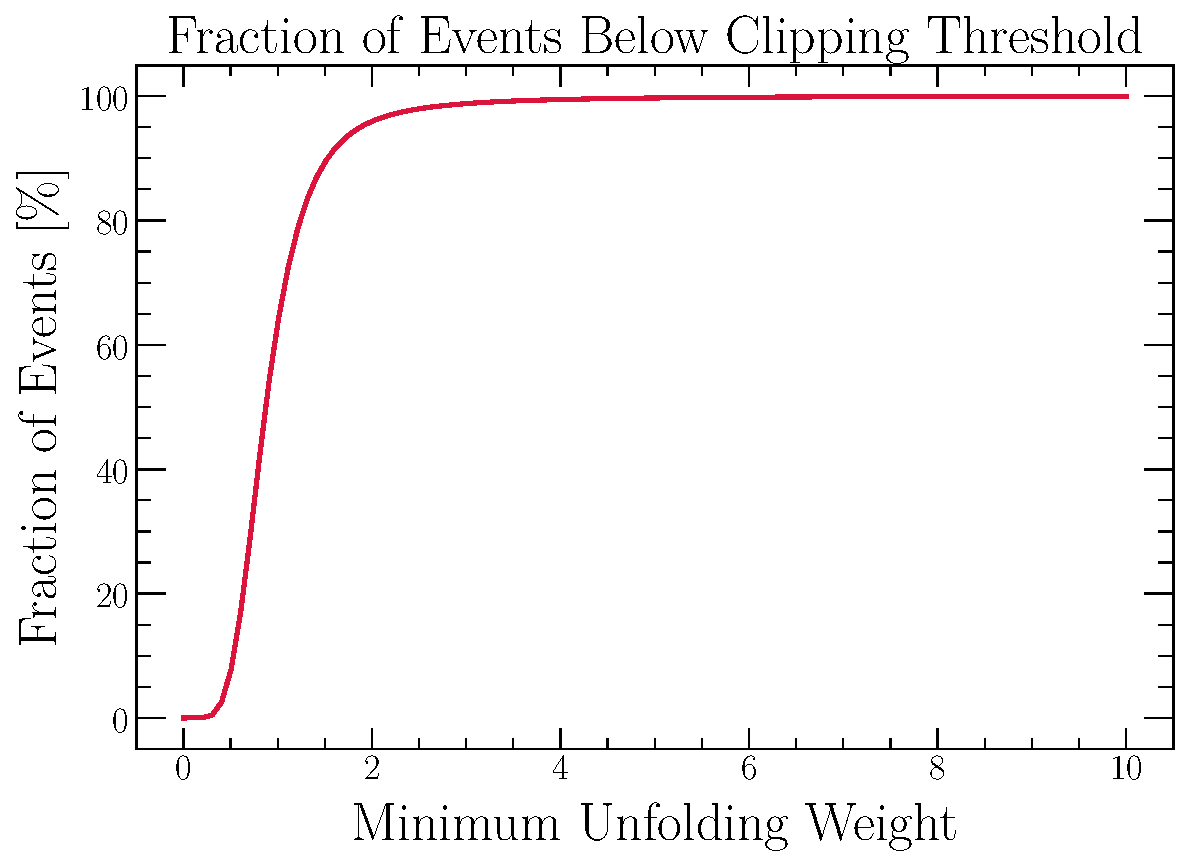
\includegraphics[width=0.95\textwidth]{figures/clipping.pdf}\\
\caption{The fraction of events with MultiFold weights that fall below a given threshold. The vast majority of weights fall between 0 and 2, and a negligible number have a magnitude larger than 10. Our applied upper limit of 100 is therefore more than sufficient to capture the full performance of MultiFold while remaining robust against very rare occurrences of infinite weights.}
\label{fig:clipping}
\end{figure}


\subsection{Technical Closure Test}
\label{sec:technicalclosure}

As a technical closure test, we unfold Pythia with itself.  To do this, we take the Pythia sample and randomly label half as `data' and the other half as `simulation'.   The unfolding should converge after one step because the Step 1 and thus Step 2 weights should all be unity.  This is shown for individual observable unfoldings in Sec.~\ref{sec:technicalclosure:unifold} and for multidimensional unfolding in Sec.~\ref{sec:technicalclosure:multifold}.

\subsubsection{UniFold}
\label{sec:technicalclosure:unifold}

Figures~\ref{fig:technicalclosure:mass},~\ref{fig:technicalclosure:ntracksjet1},~\ref{fig:technicalclosure:pT_trackj1},~\ref{fig:technicalclosure:tau1_trackj1}, and~\ref{fig:technicalclosure:y_trackj1} show the technical closure of UniFold for the leading track jet mass, constituent multiplicity, $p_T$, $\tau_1$ and rapidity, respectively.  In all cases, the unfolding converges after one iteration, as expected.

\begin{figure}[h!]
\centering
\subfloat[Input histograms]{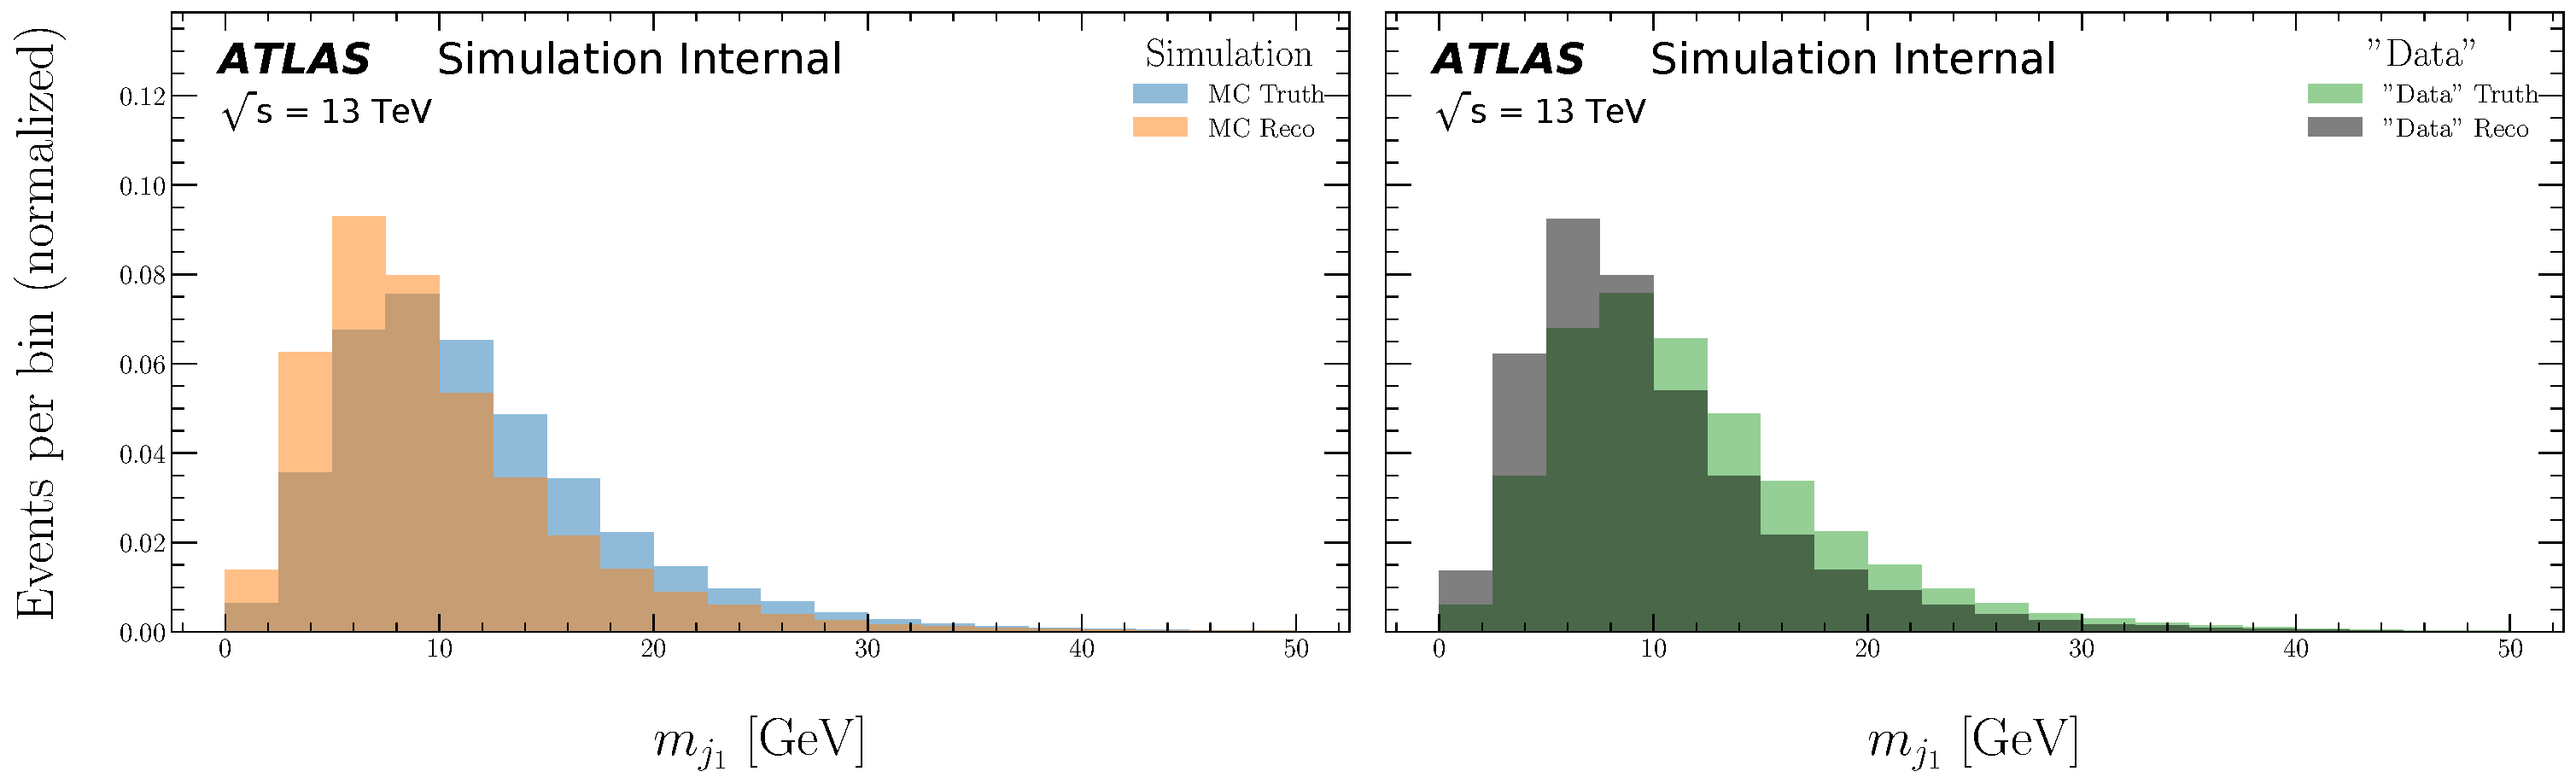
\includegraphics[width=0.95\textwidth]{figures/ATLASOmniFold-StressTest/ATLASOmniFold-TechnicalClosureTest/UniFold/m_trackj1/ATLASOmniFold-TechnicalClosureTest-UniFold-m_trackj1-Distributions.pdf}}\\
\subfloat[After 1 iteration]{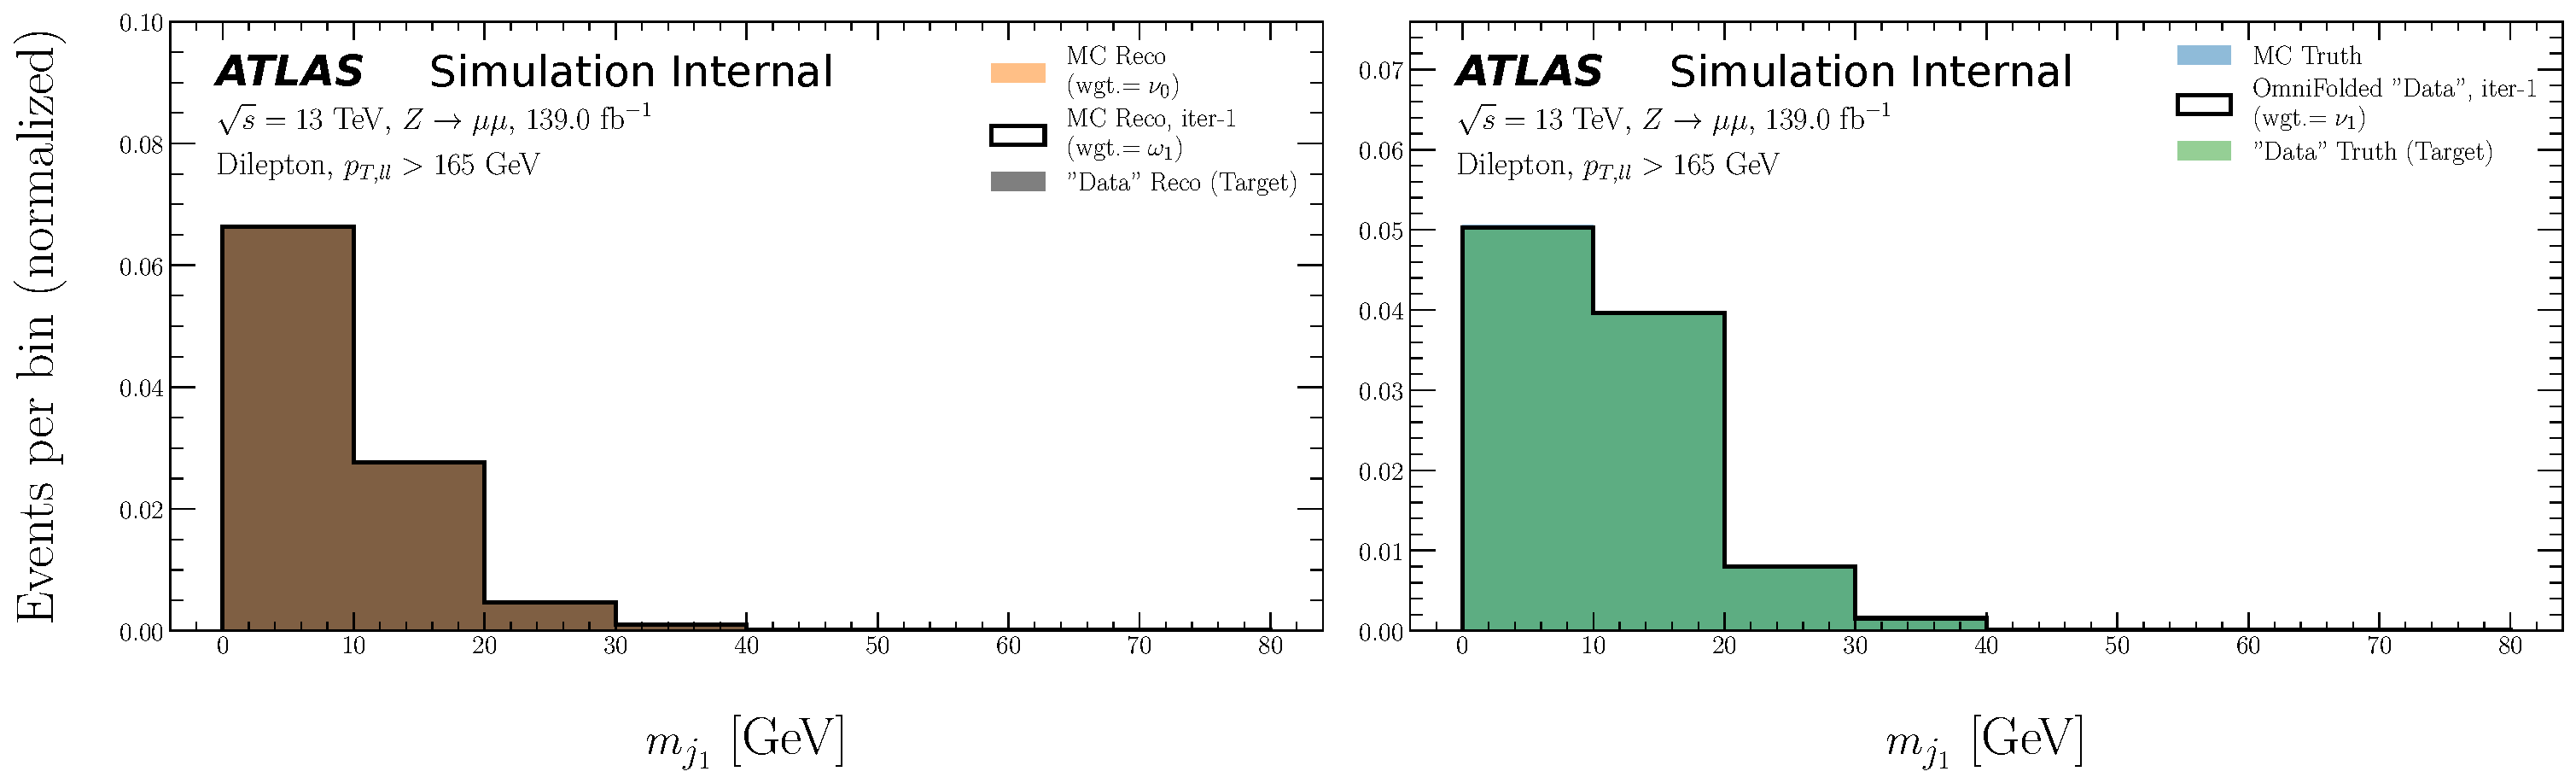
\includegraphics[width=0.95\textwidth]{figures/ATLASOmniFold-StressTest/ATLASOmniFold-TechnicalClosureTest/UniFold/m_trackj1/ATLASOmniFold-TechnicalClosureTest-UniFold-m_trackj1-Iteration01.pdf}}
\caption{A technical closure test for the mass of the leading track jet using using UniFold.  The top plot show the input histograms and the bottom plots are the results after one iteration of OmniFold.  By construction the top left and top right histograms are statistically identical.}
\label{fig:technicalclosure:mass}
\end{figure}

\begin{figure}[h!]
\centering
\subfloat[Input histograms]{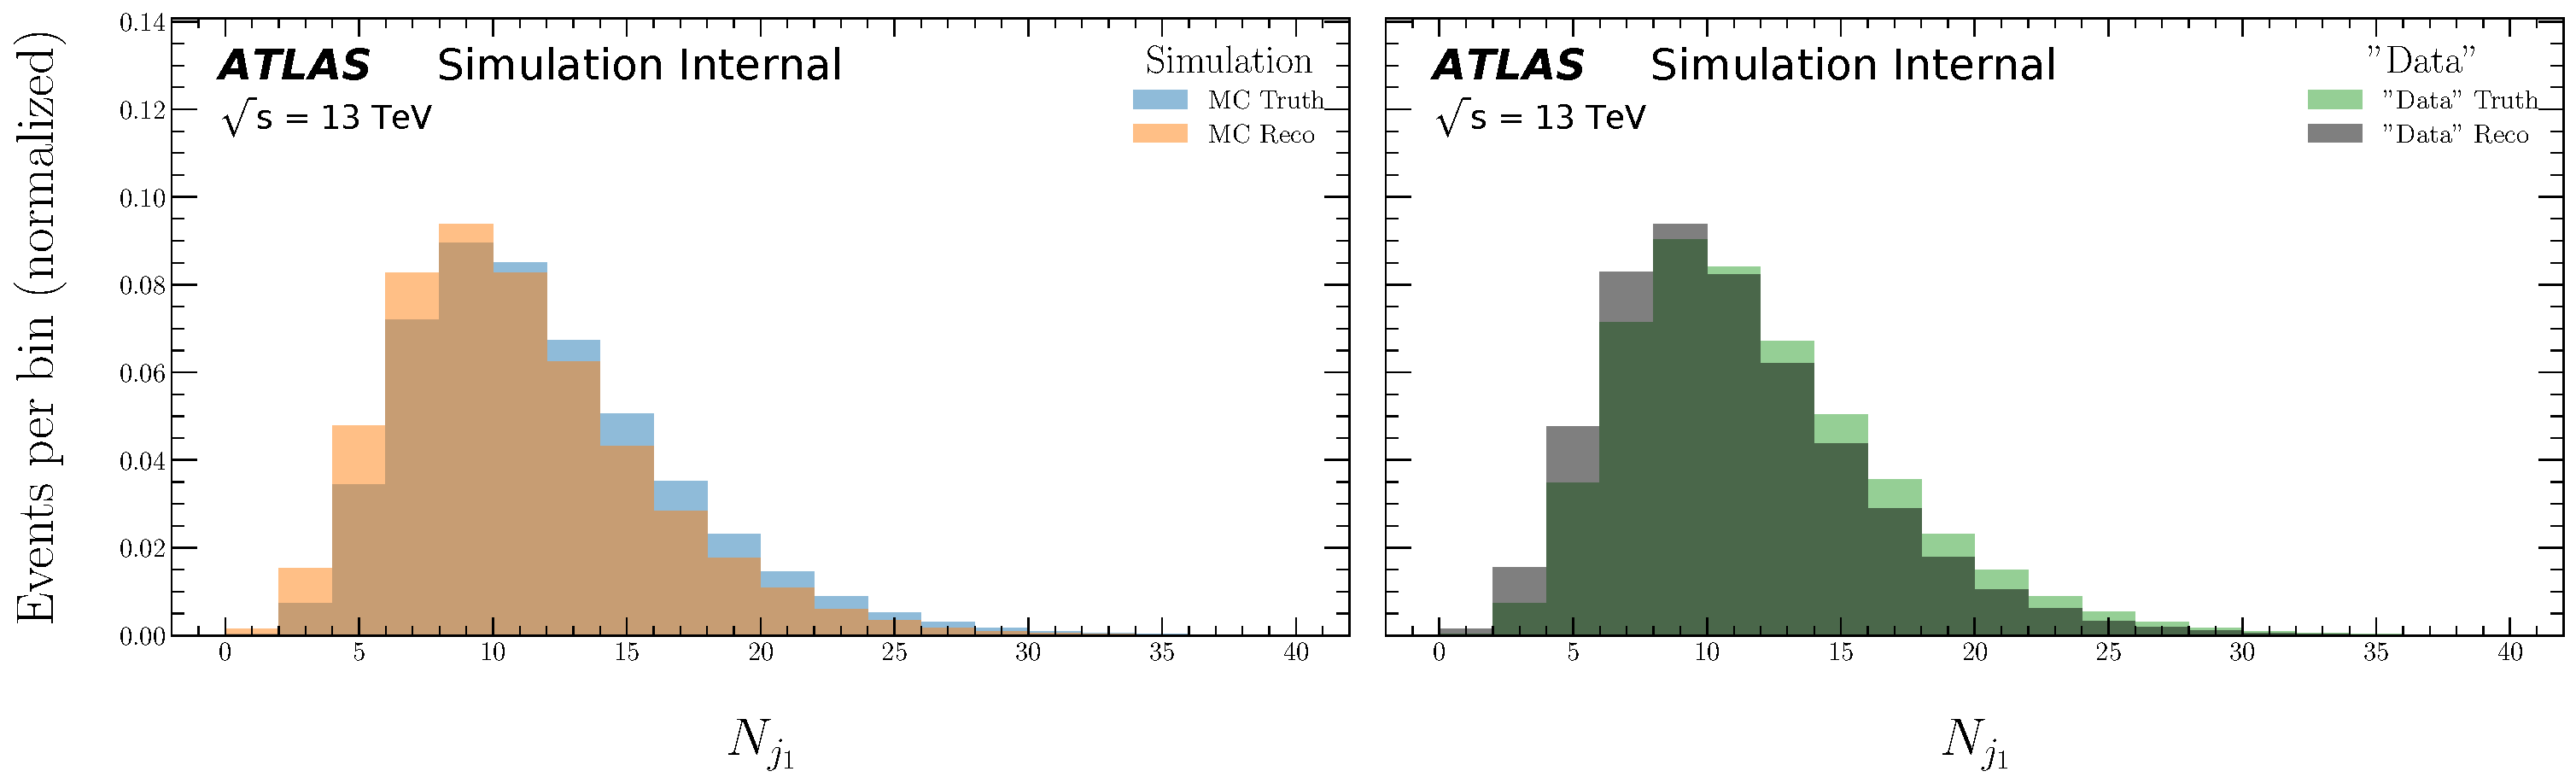
\includegraphics[width=0.95\textwidth]{figures/ATLASOmniFold-StressTest/ATLASOmniFold-TechnicalClosureTest/UniFold/Ntracks_trackj1/ATLASOmniFold-TechnicalClosureTest-UniFold-Ntracks_trackj1-Distributions.pdf}}\\
\subfloat[After 1 iteration]{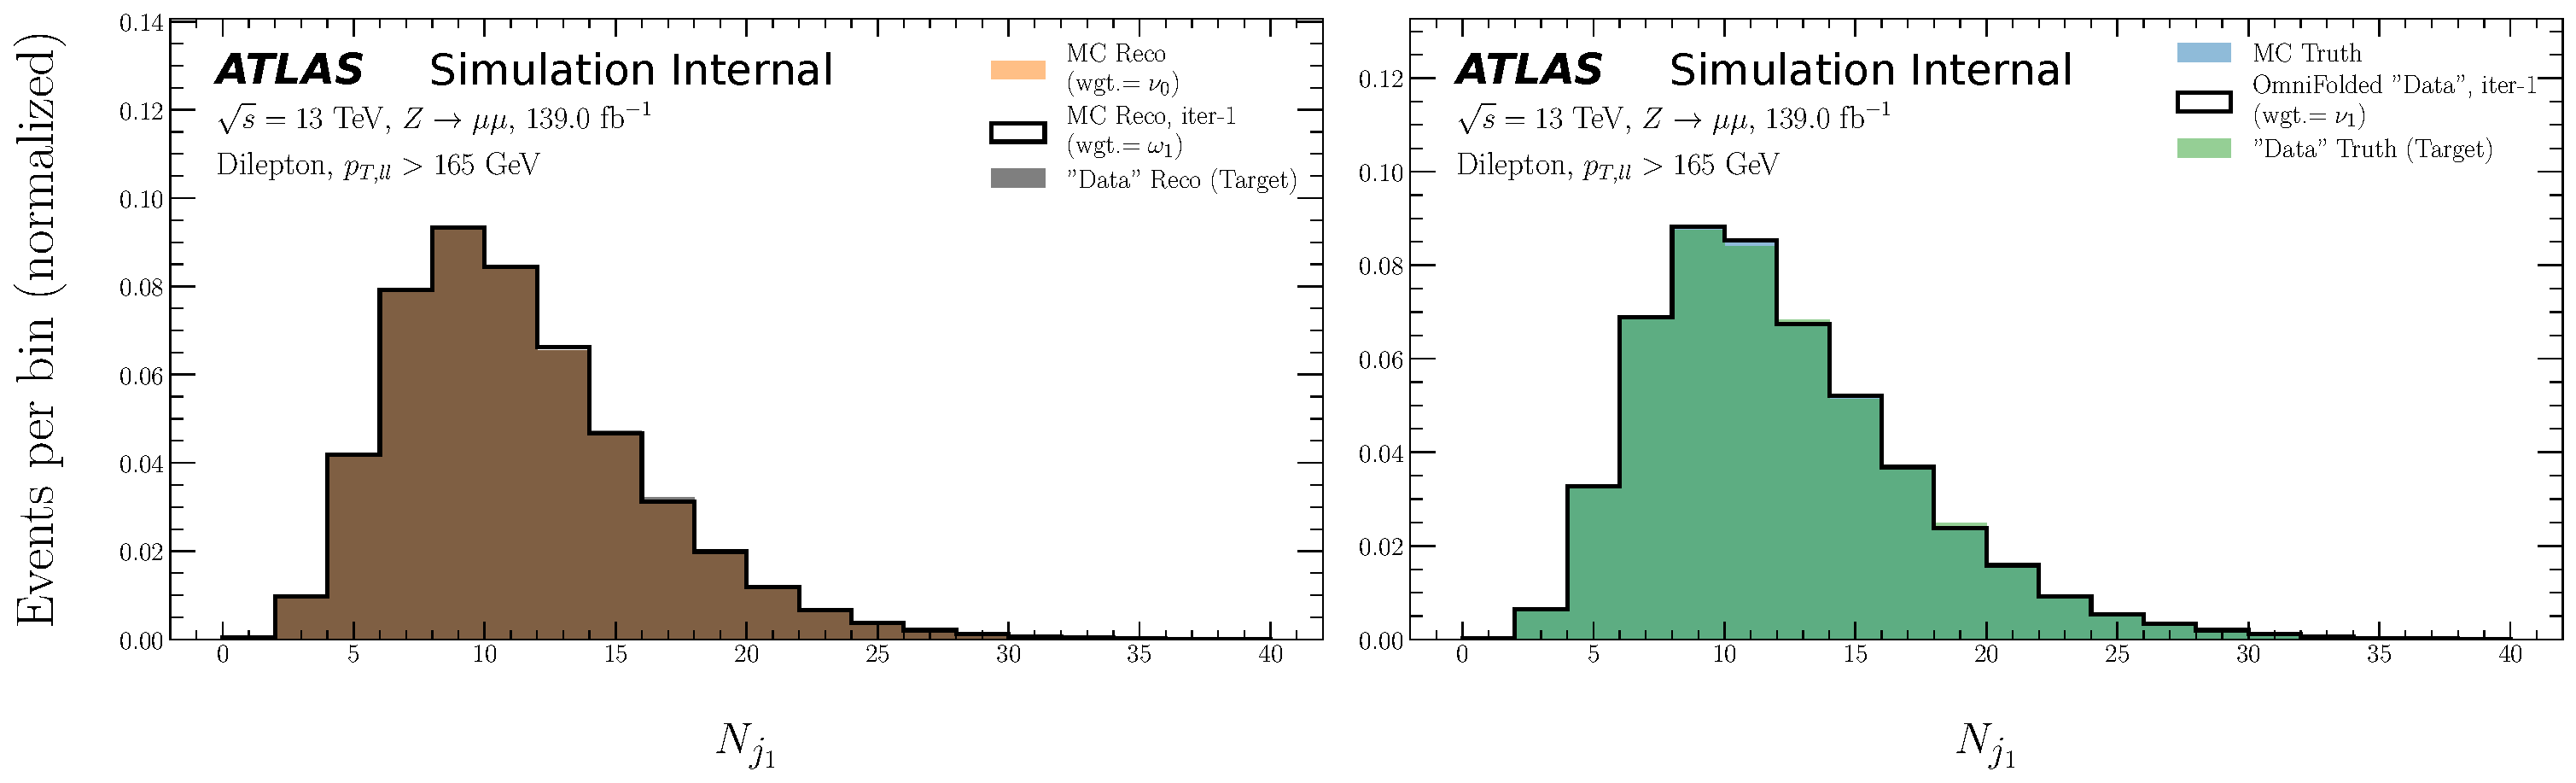
\includegraphics[width=0.95\textwidth]{figures/ATLASOmniFold-StressTest/ATLASOmniFold-TechnicalClosureTest/UniFold/Ntracks_trackj1/ATLASOmniFold-TechnicalClosureTest-UniFold-Ntracks_trackj1-Iteration01.pdf}}
\caption{A technical closure test for the number of tracks in the leading track jet using UniFold.  The top plot show the input histograms and the bottom plots are the results after one iteration of OmniFold.  By construction the top left and top right histograms are statistically identical.}
\label{fig:technicalclosure:ntracksjet1}
\end{figure}

\begin{figure}[h!]
\centering
\subfloat[Input histograms]{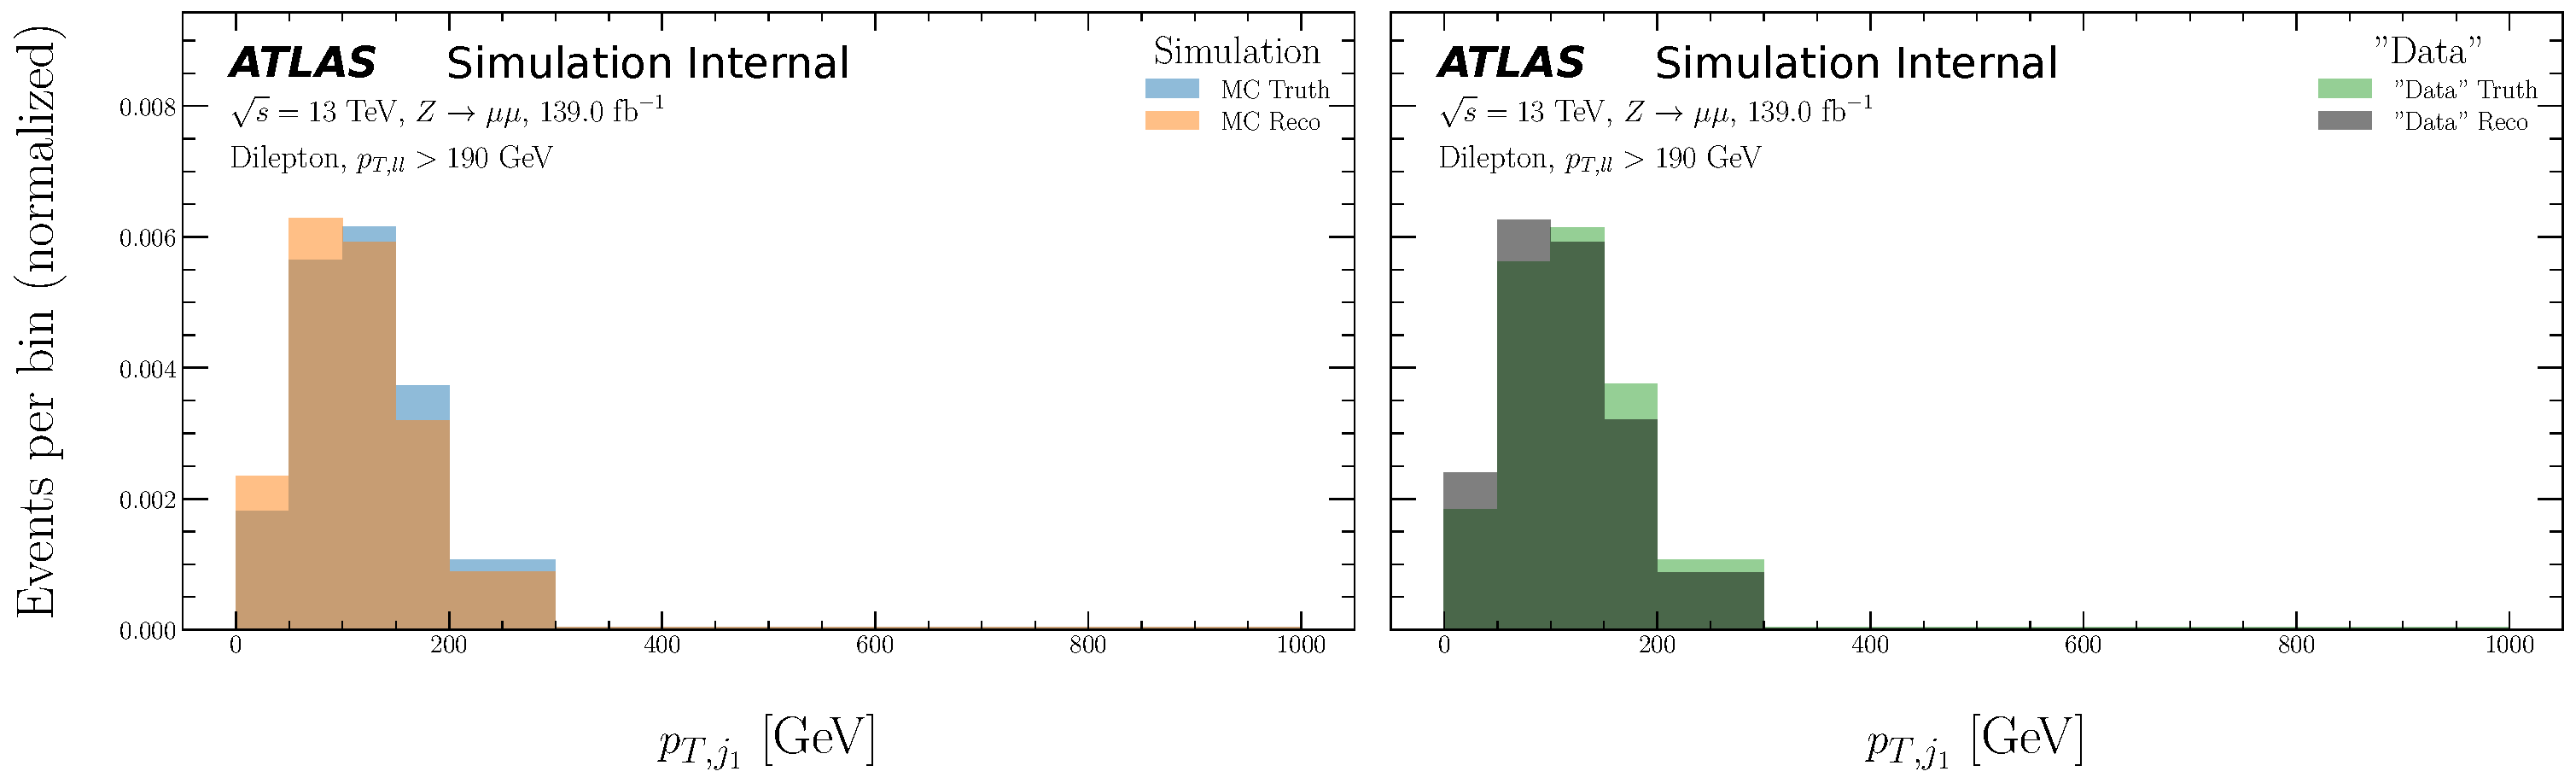
\includegraphics[width=0.95\textwidth]{figures/ATLASOmniFold-StressTest/ATLASOmniFold-TechnicalClosureTest/UniFold/pT_trackj1/ATLASOmniFold-TechnicalClosureTest-UniFold-pT_trackj1-Distributions.pdf}}\\
\subfloat[After 1 iteration]{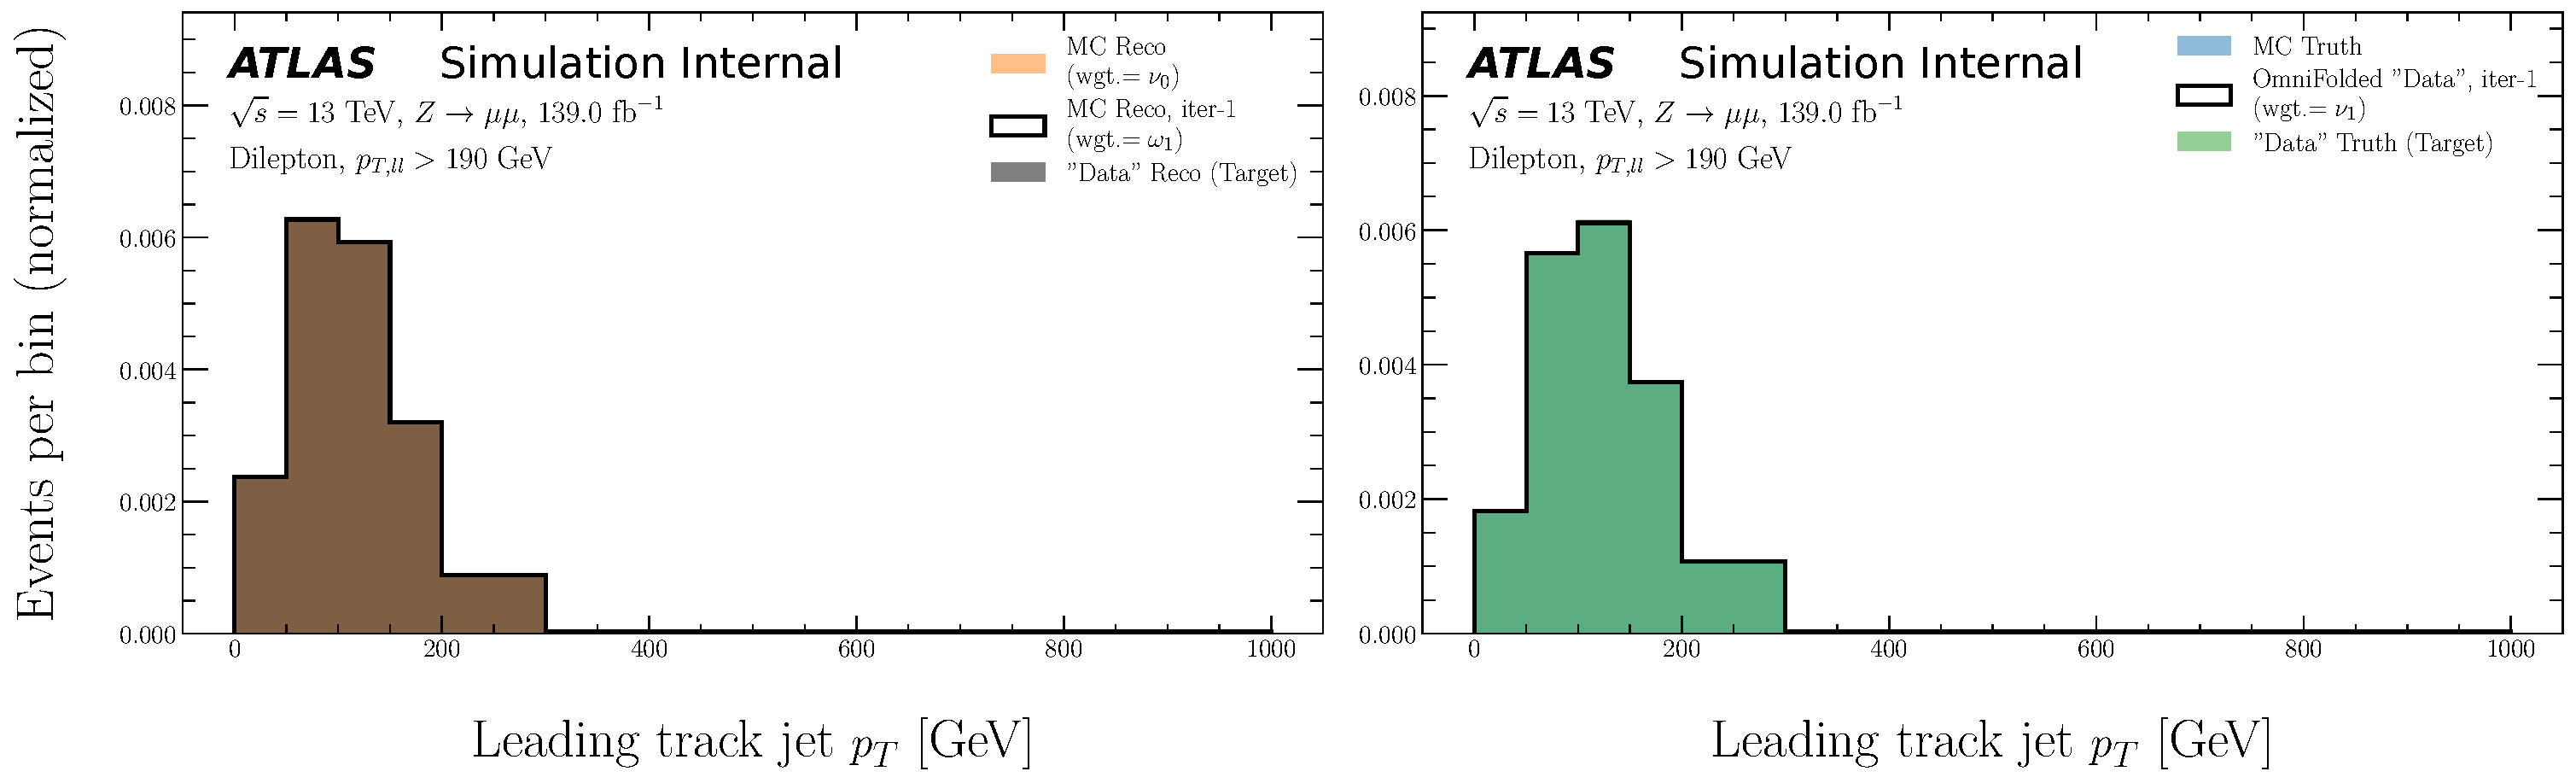
\includegraphics[width=0.95\textwidth]{figures/ATLASOmniFold-StressTest/ATLASOmniFold-TechnicalClosureTest/UniFold/pT_trackj1/ATLASOmniFold-TechnicalClosureTest-UniFold-pT_trackj1-Iteration01.pdf}}
\caption{A technical closure test for the $p_T$ of the leading track jet using UniFold.  The top plot show the input histograms and the bottom plots are the results after one iteration of OmniFold.  By construction the top left and top right histograms are statistically identical.}
\label{fig:technicalclosure:pT_trackj1}
\end{figure}

\begin{figure}[h!]
\centering
\subfloat[Input histograms]{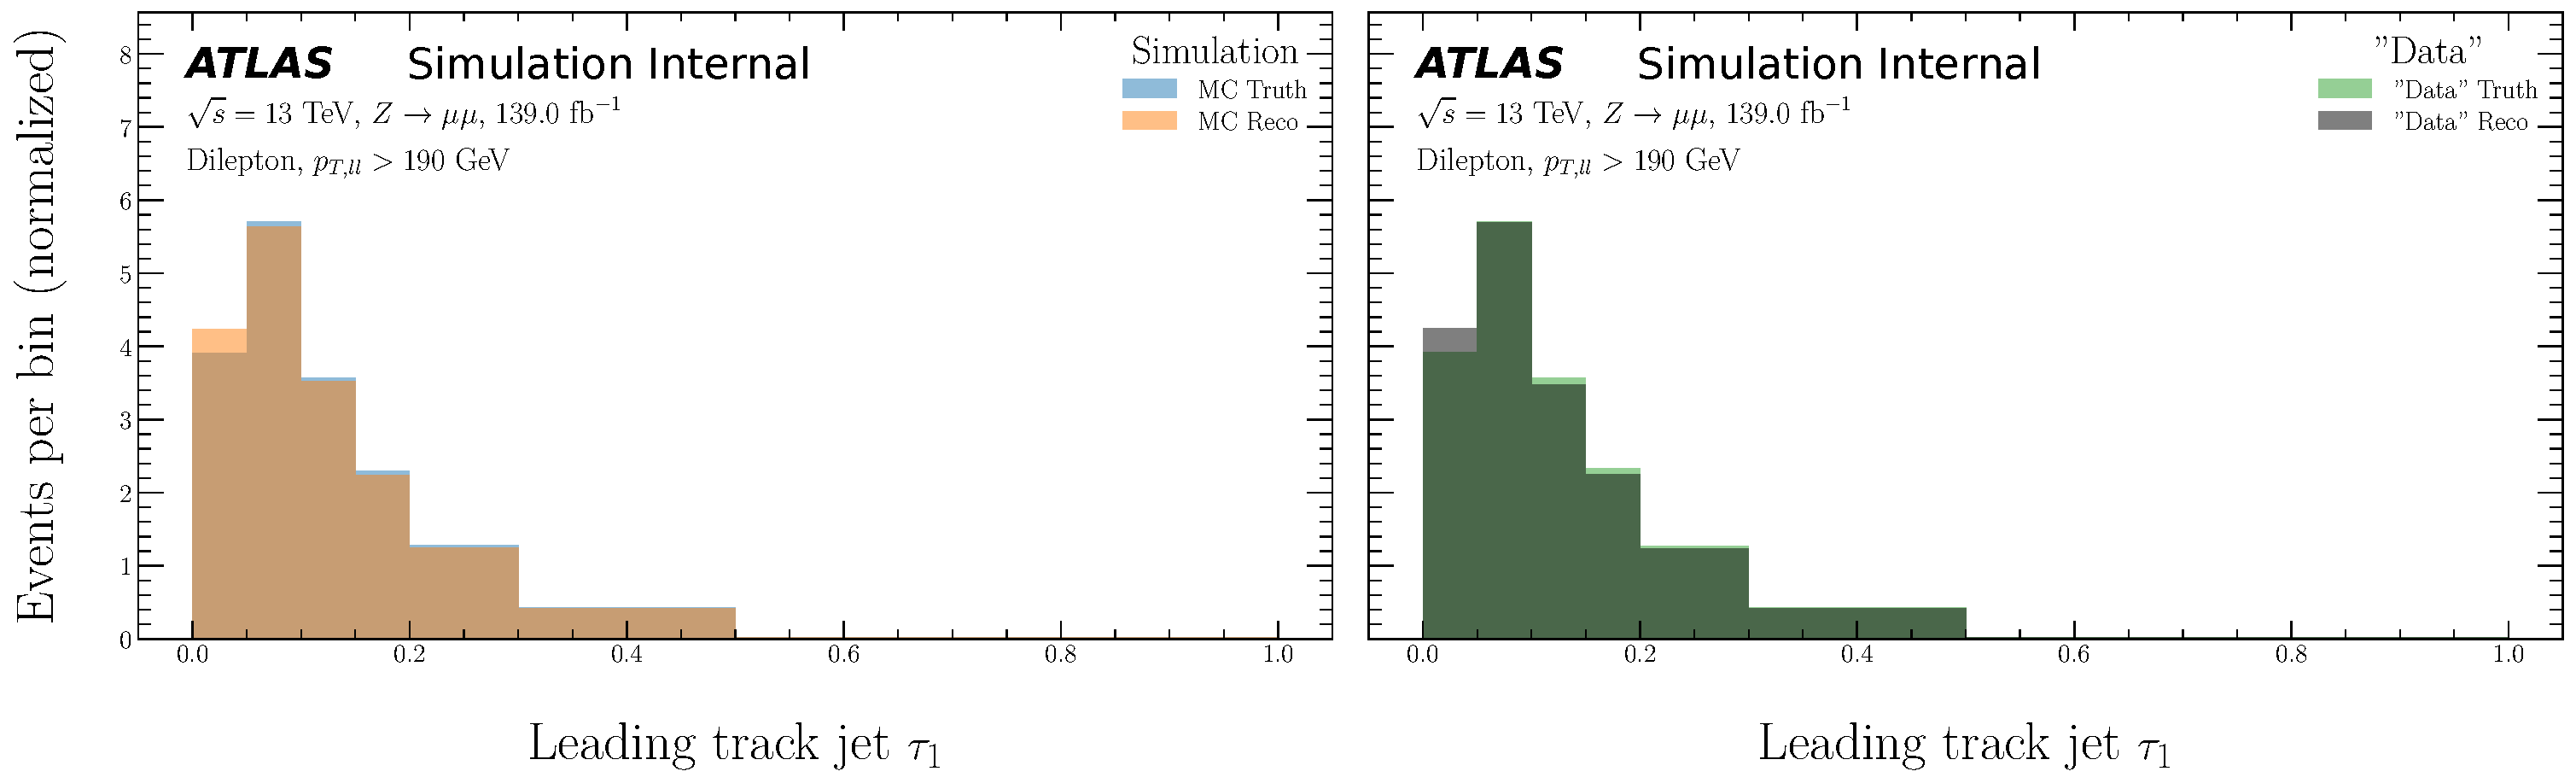
\includegraphics[width=0.89\textwidth]{figures/ATLASOmniFold-StressTest/ATLASOmniFold-TechnicalClosureTest/UniFold/tau1_trackj1/ATLASOmniFold-TechnicalClosureTest-UniFold-tau1_trackj1-Distributions.pdf}}\\
\subfloat[After 1 iteration]{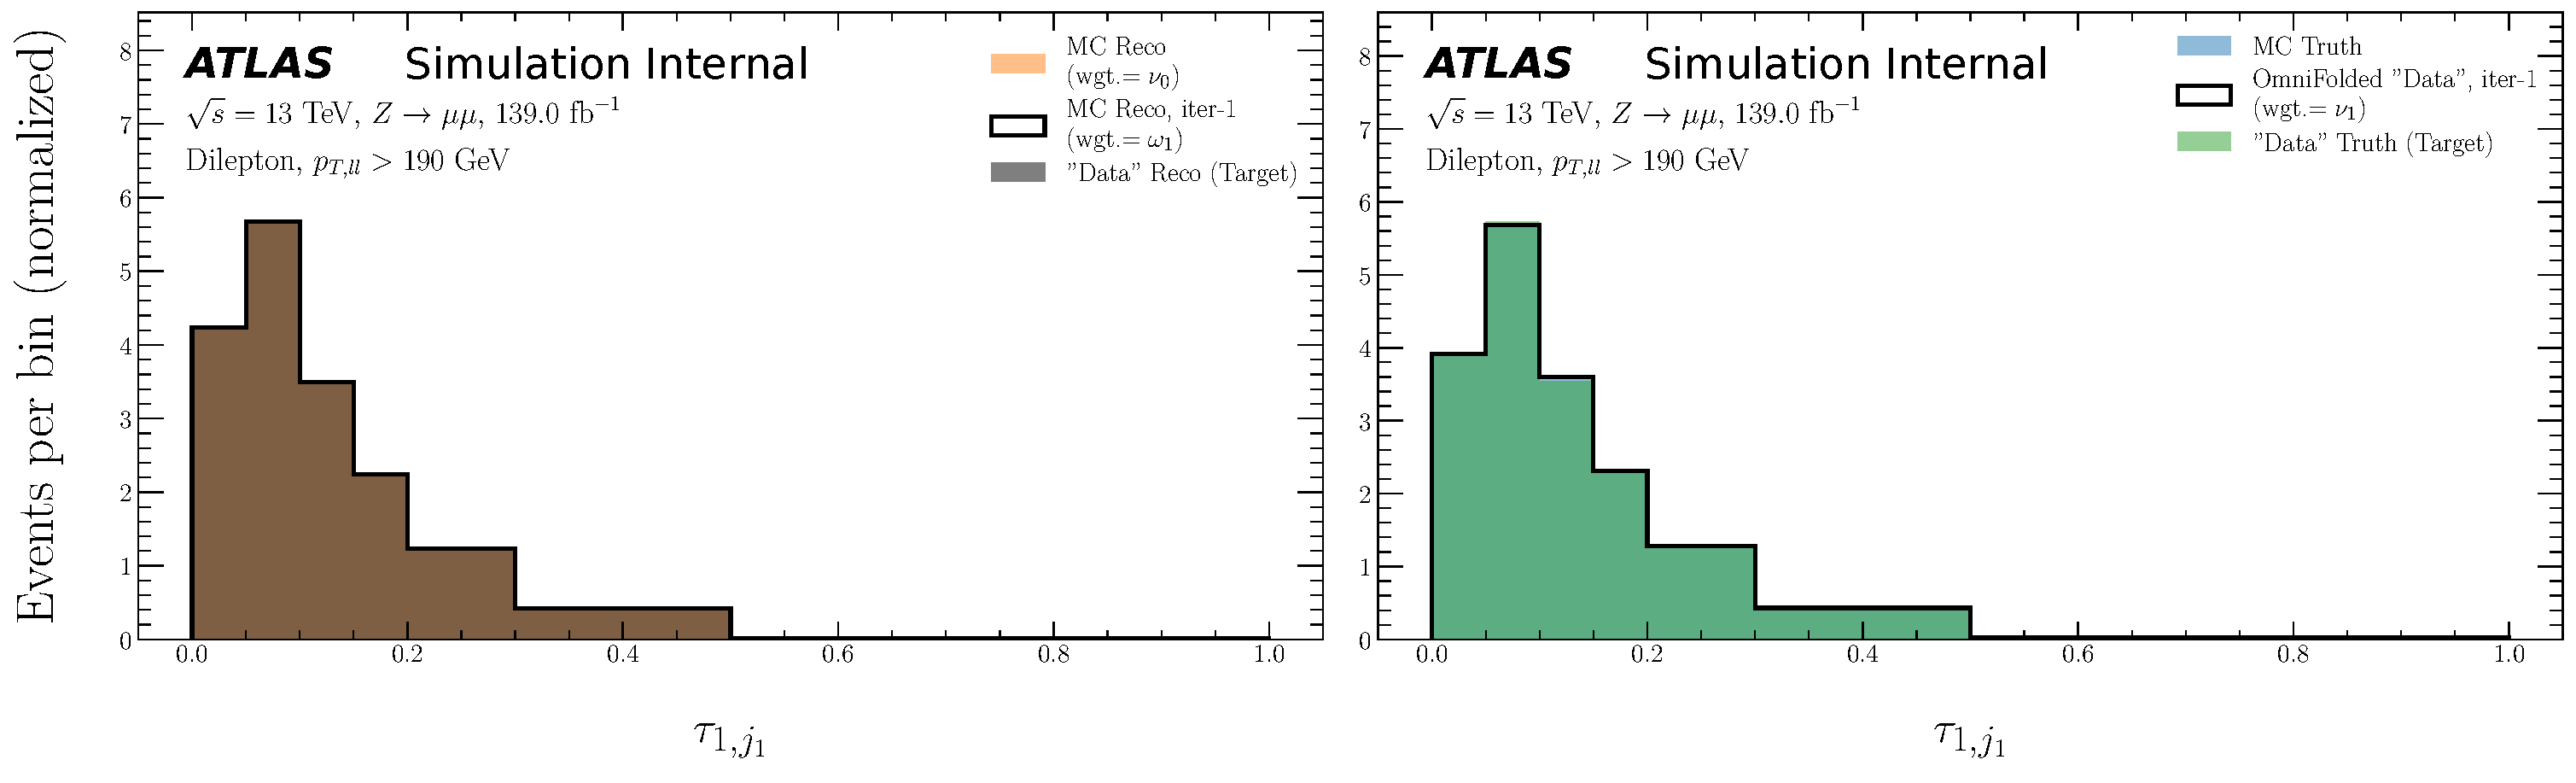
\includegraphics[width=0.95\textwidth]{figures/ATLASOmniFold-StressTest/ATLASOmniFold-TechnicalClosureTest/UniFold/tau1_trackj1/ATLASOmniFold-TechnicalClosureTest-UniFold-tau1_trackj1-Iteration01.pdf}}
\caption{A technical closure test for the $\tau_1$ of the leading track jet using UniFold.  The top plot show the input histograms and the bottom plots are the results after one iteration of OmniFold.  By construction the top left and top right histograms are statistically identical.}
\label{fig:technicalclosure:tau1_trackj1}
\end{figure}

\begin{figure}[h!]
\centering
\subfloat[Input histograms]{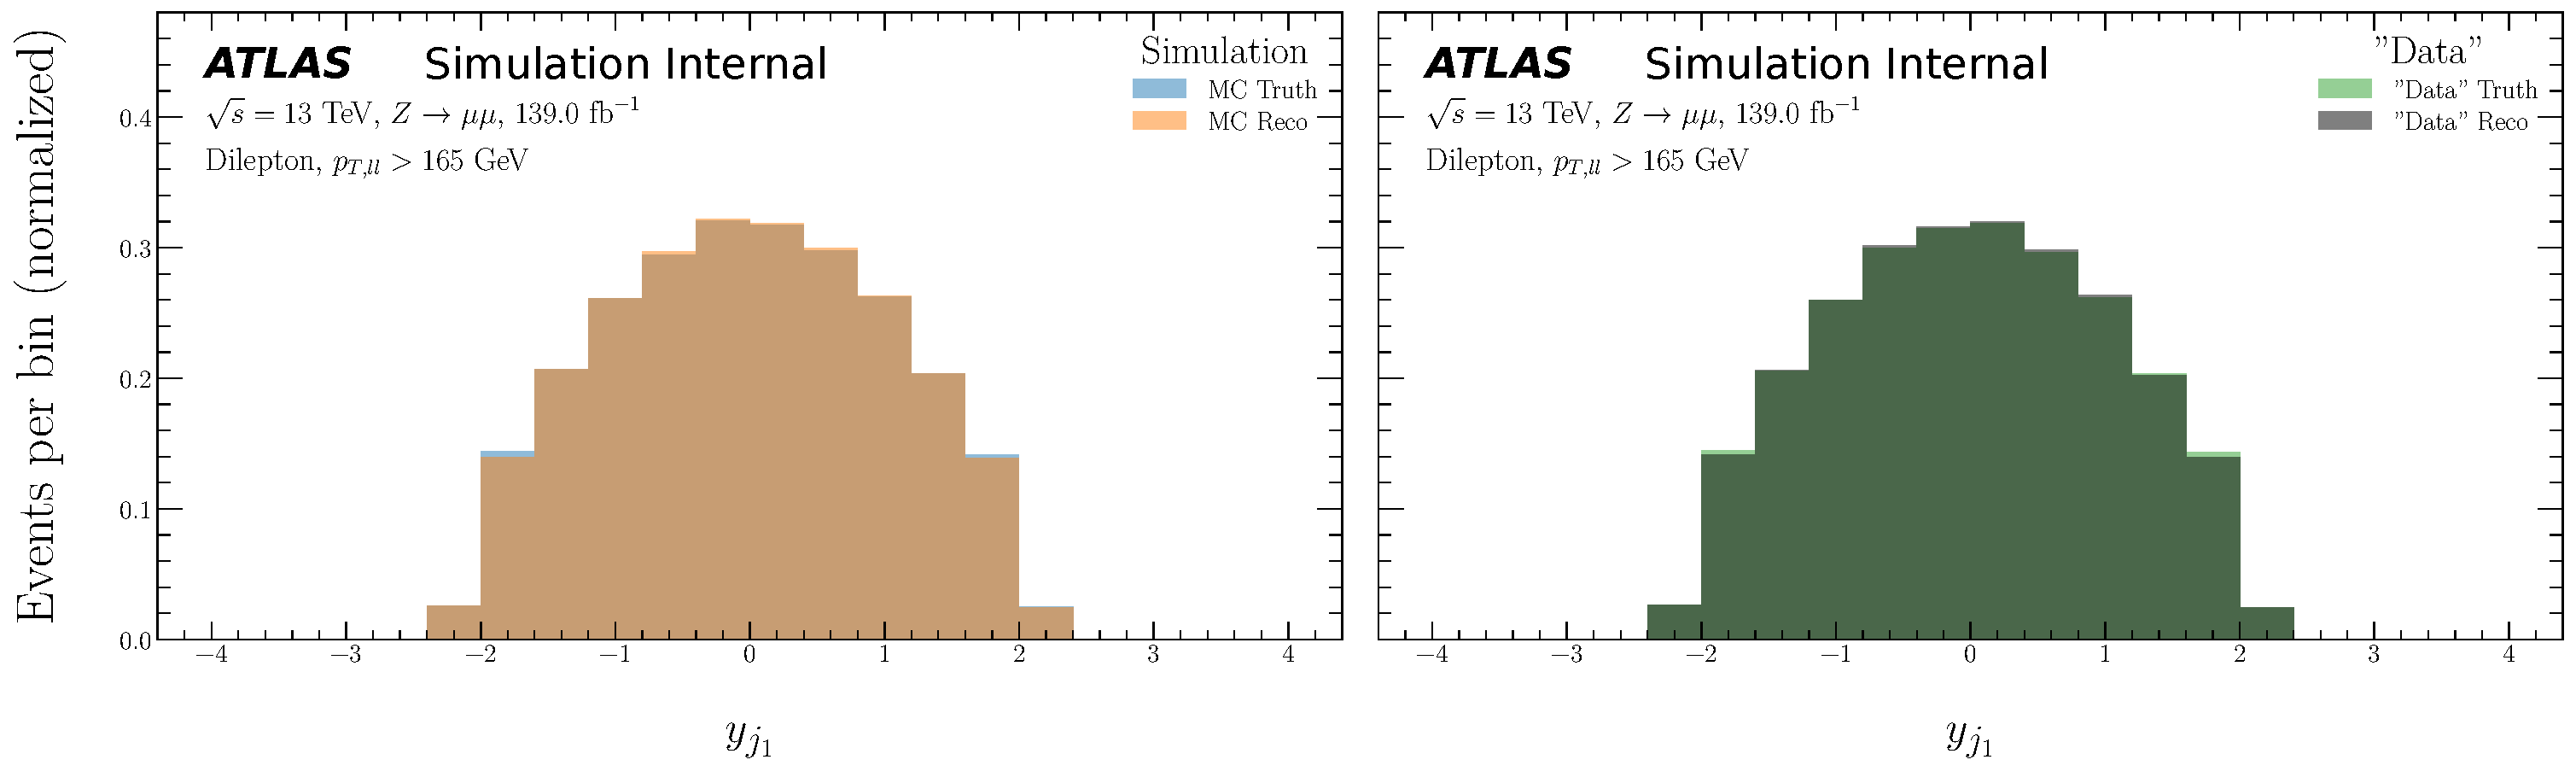
\includegraphics[width=0.95\textwidth]{figures/ATLASOmniFold-StressTest/ATLASOmniFold-TechnicalClosureTest/UniFold/y_trackj1/ATLASOmniFold-TechnicalClosureTest-UniFold-y_trackj1-Distributions.pdf}}\\
\subfloat[After 1 iteration]{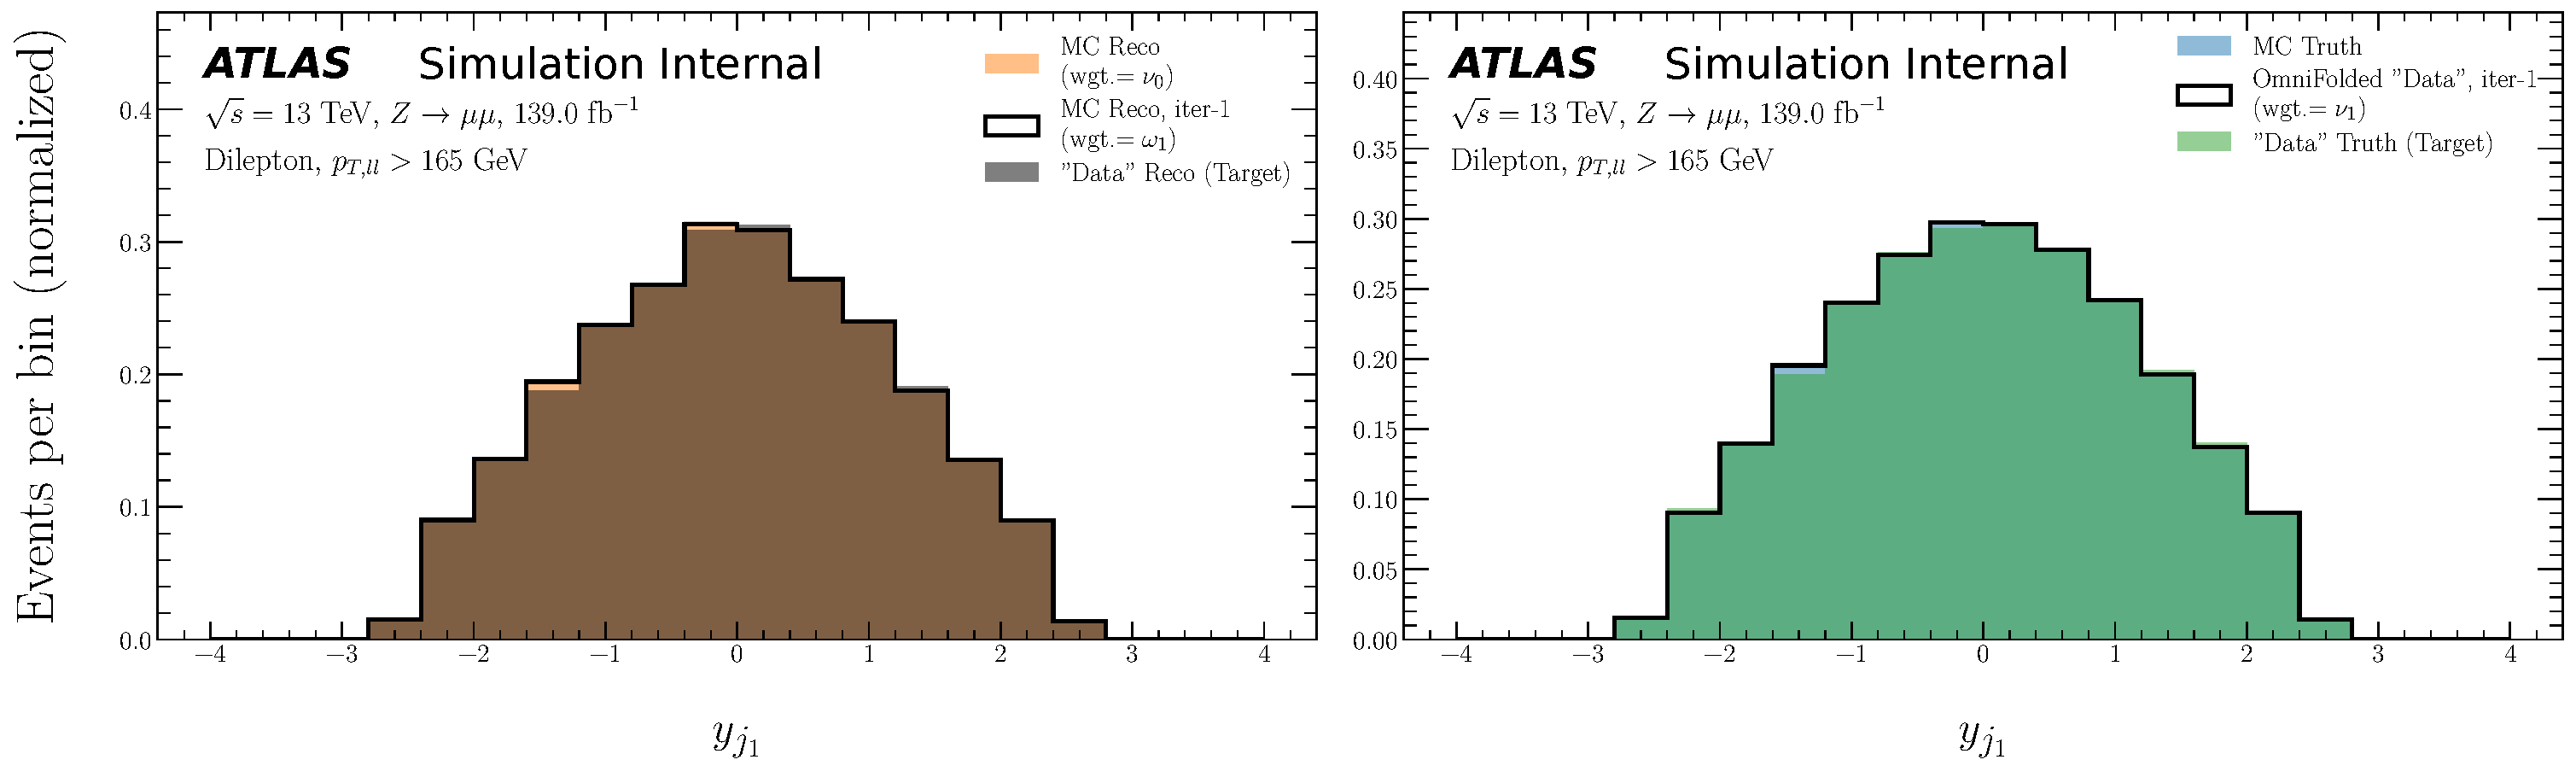
\includegraphics[width=0.95\textwidth]{figures/ATLASOmniFold-StressTest/ATLASOmniFold-TechnicalClosureTest/UniFold/y_trackj1/ATLASOmniFold-TechnicalClosureTest-UniFold-y_trackj1-Iteration01.pdf}}
\caption{A technical closure test for the rapidity of the leading track jet using UniFold.  The top plot show the input histograms and the bottom plots are the results after one iteration of OmniFold.  By construction the top left and top right histograms are statistically identical.}
\label{fig:technicalclosure:y_trackj1}
\end{figure}

\subsubsection{MultiFold}
\label{sec:technicalclosure:multifold}

In this section, we determine the closure of a 16-dimensional unfolding that includes $\pt^{\mu\mu}$, $y_{\mu\mu}$ and the following properties of the leading and subleading track jets: mass, constituent multiplicity, $\pt$, rapidity, $\phi$, $\tau_1$, $\tau_2$, and $\tau_3$.  For illustration, the same five observables as in Sec.~\ref{sec:technicalclosure:unifold} are shown in figures~\ref{fig:technicalclosureMulti:mass},~\ref{fig:technicalclosureMulti:ntracksjet1},~\ref{fig:technicalclosureMulti:pT_trackj1},~\ref{fig:technicalclosureMulti:tau1_trackj1}, and~\ref{fig:technicalclosureMulti:y_trackj1}, but the quality of the technical closure is excellent for any projection of the 16-dimensional space (the remaining 11 observables histograms are in App.~\ref{sec:multifoldtechnicalclosure}).

\begin{figure}[h!]
\centering
\subfloat[Input histograms]{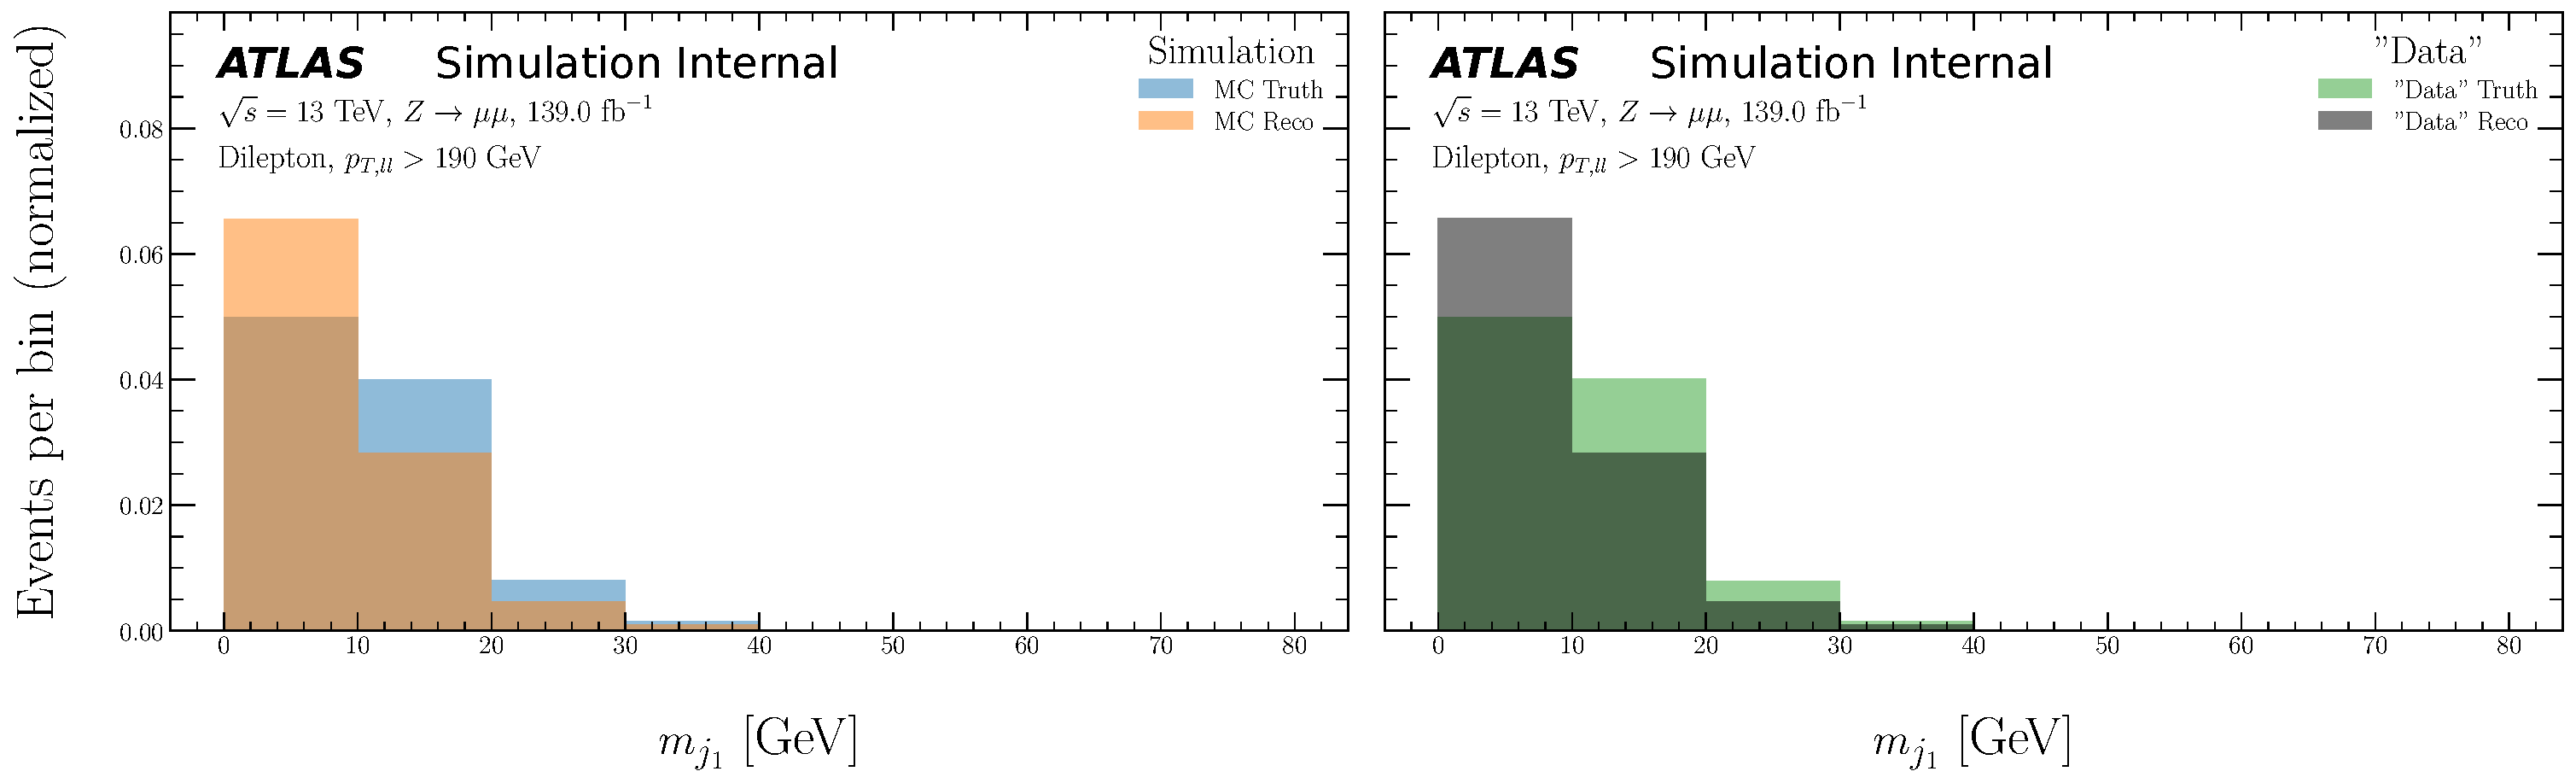
\includegraphics[width=0.95\textwidth]{figures/ATLASOmniFold-StressTest/ATLASOmniFold-TechnicalClosureTest/MultiFold/m_trackj1/ATLASOmniFold-TechnicalClosureTest-MultiFold-m_trackj1-Distributions.pdf}}\\
\subfloat[After 1 iteration]{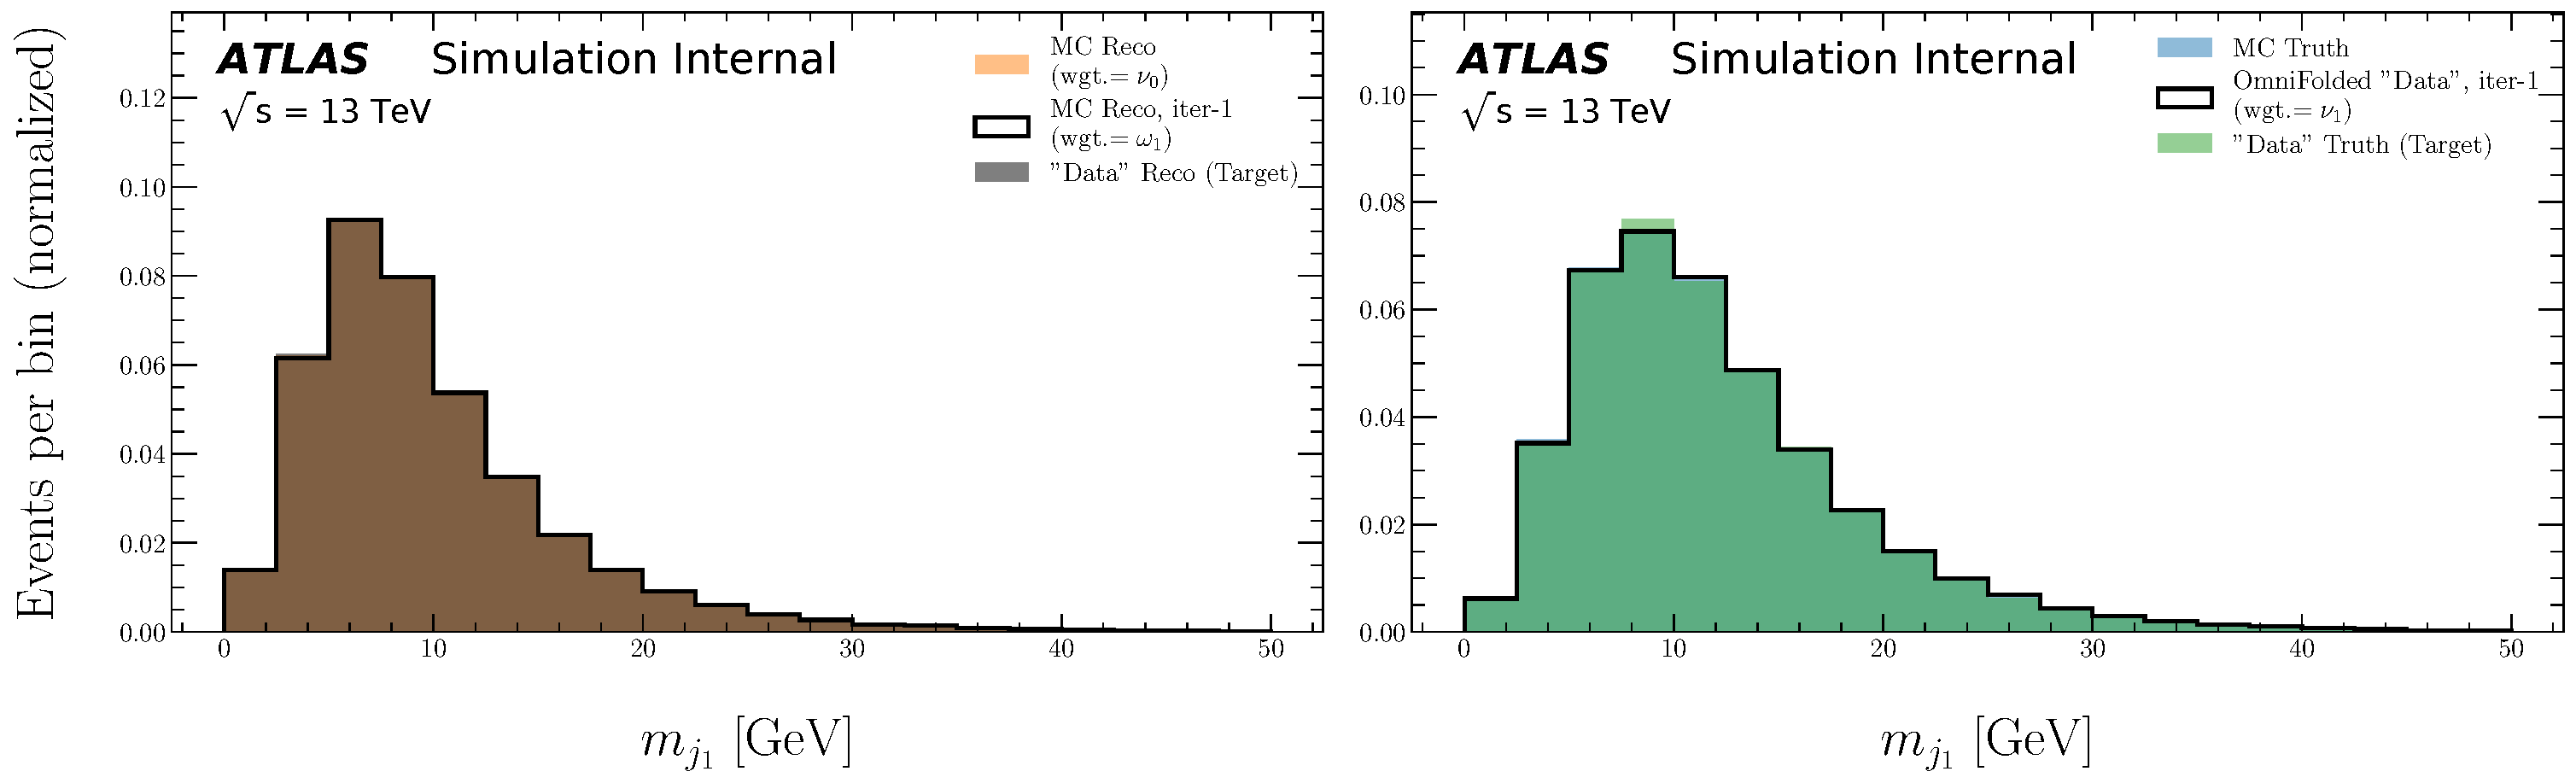
\includegraphics[width=0.95\textwidth]{figures/ATLASOmniFold-StressTest/ATLASOmniFold-TechnicalClosureTest/MultiFold/m_trackj1/ATLASOmniFold-TechnicalClosureTest-MultiFold-m_trackj1-Iteration01.pdf}}
\caption{A technical closure test for the mass of the leading track jet using using MultiFold (16 observables are simultaneously unfolded).  The top plot show the input histograms and the bottom plots are the results after one iteration of OmniFold.  By construction the top left and top right histograms are statistically identical.}
\label{fig:technicalclosureMulti:mass}
\end{figure}

\begin{figure}[h!]
\centering
\subfloat[Input histograms]{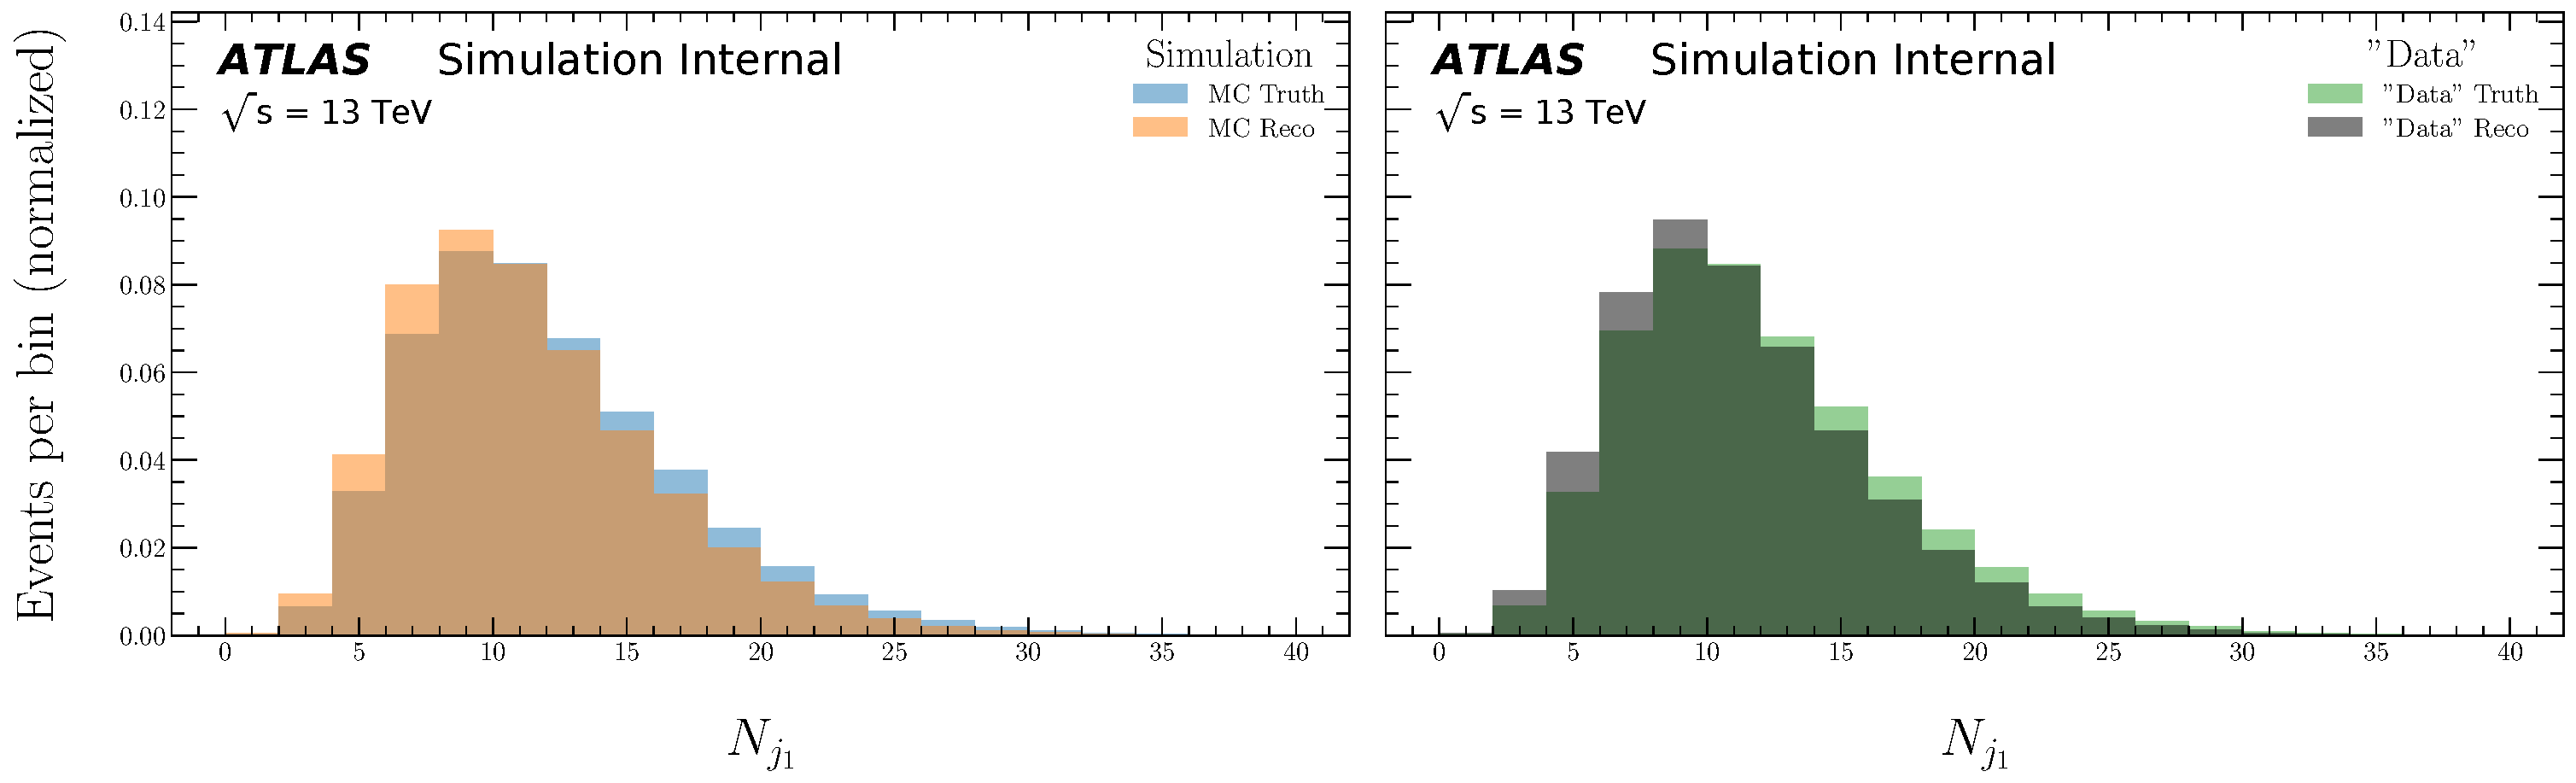
\includegraphics[width=0.95\textwidth]{figures/ATLASOmniFold-StressTest/ATLASOmniFold-TechnicalClosureTest/MultiFold/Ntracks_trackj1/ATLASOmniFold-TechnicalClosureTest-MultiFold-Ntracks_trackj1-Distributions.pdf}}\\
\subfloat[After 1 iteration]{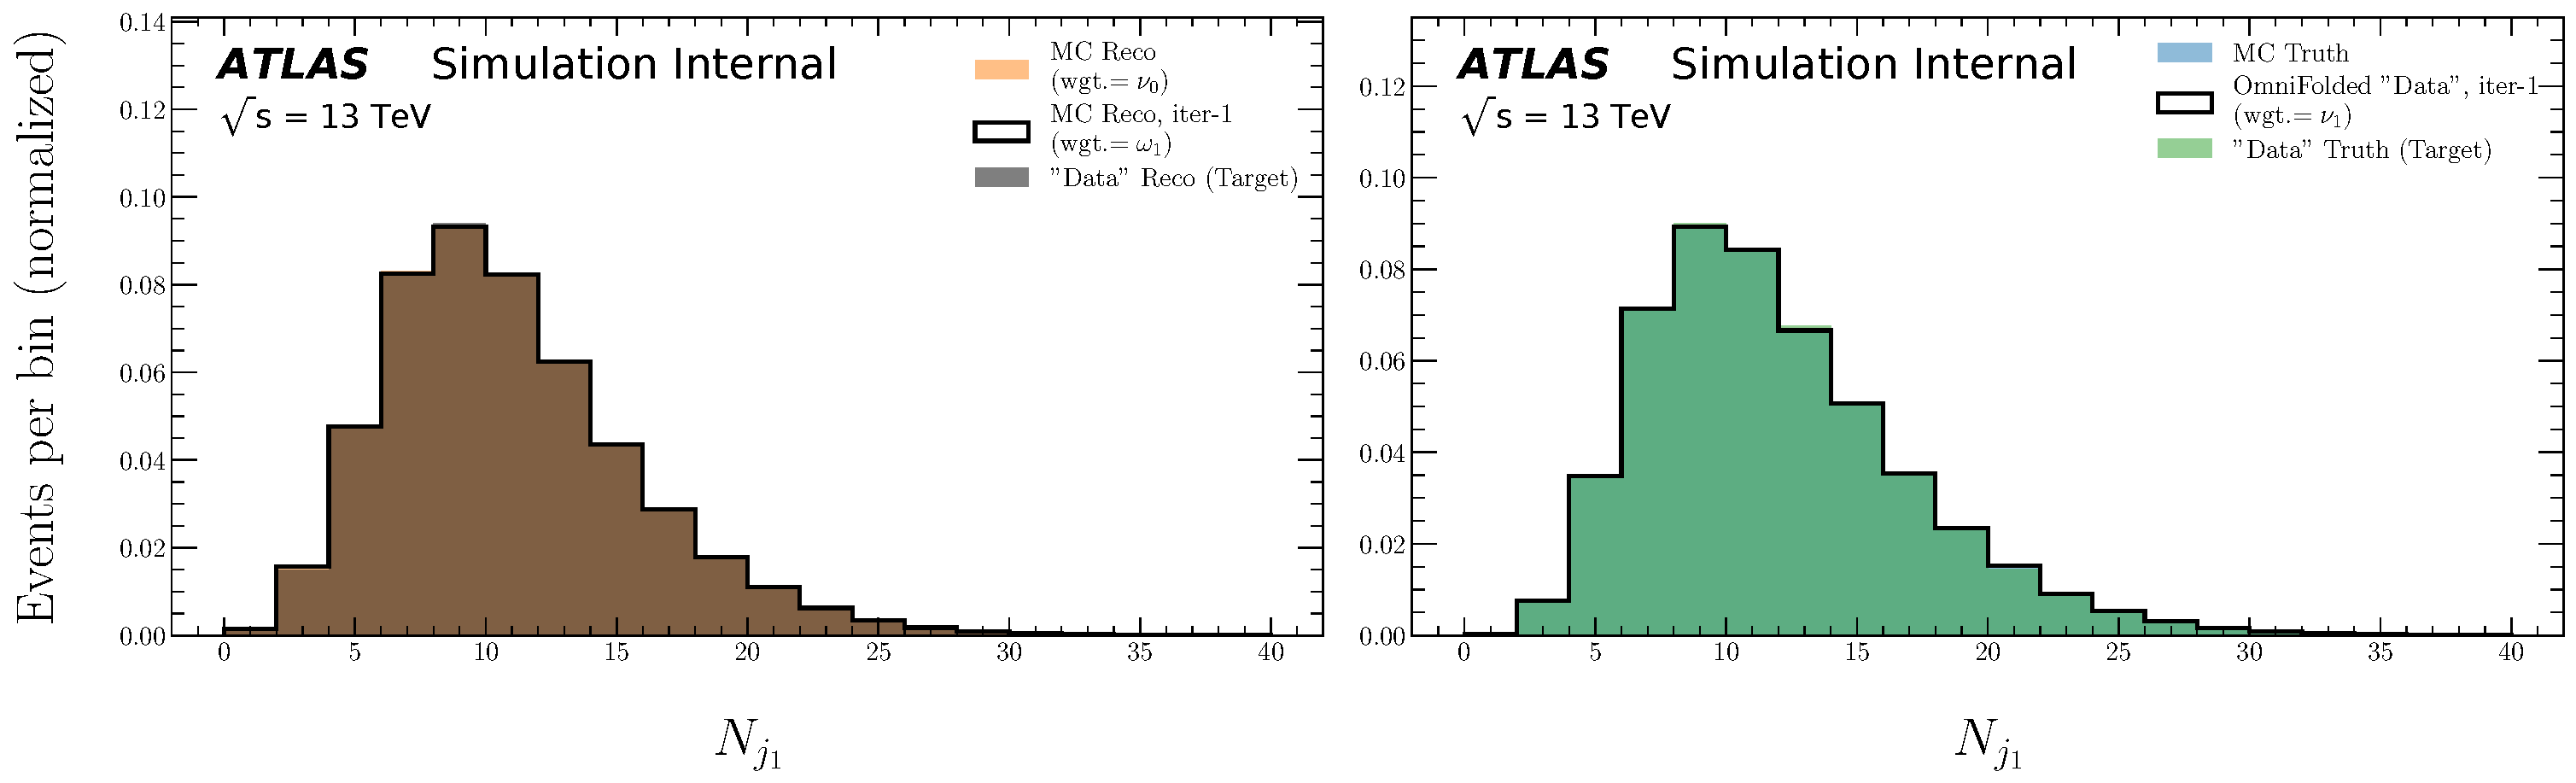
\includegraphics[width=0.95\textwidth]{figures/ATLASOmniFold-StressTest/ATLASOmniFold-TechnicalClosureTest/MultiFold/Ntracks_trackj1/ATLASOmniFold-TechnicalClosureTest-MultiFold-Ntracks_trackj1-Iteration01.pdf}}
\caption{A technical closure test for the number of tracks in the leading track jet using MultiFold (16 observables are simultaneously unfolded).  The top plot show the input histograms and the bottom plots are the results after one iteration of OmniFold.  By construction the top left and top right histograms are statistically identical.}
\label{fig:technicalclosureMulti:ntracksjet1}
\end{figure}

\begin{figure}[h!]
\centering
\subfloat[Input histograms]{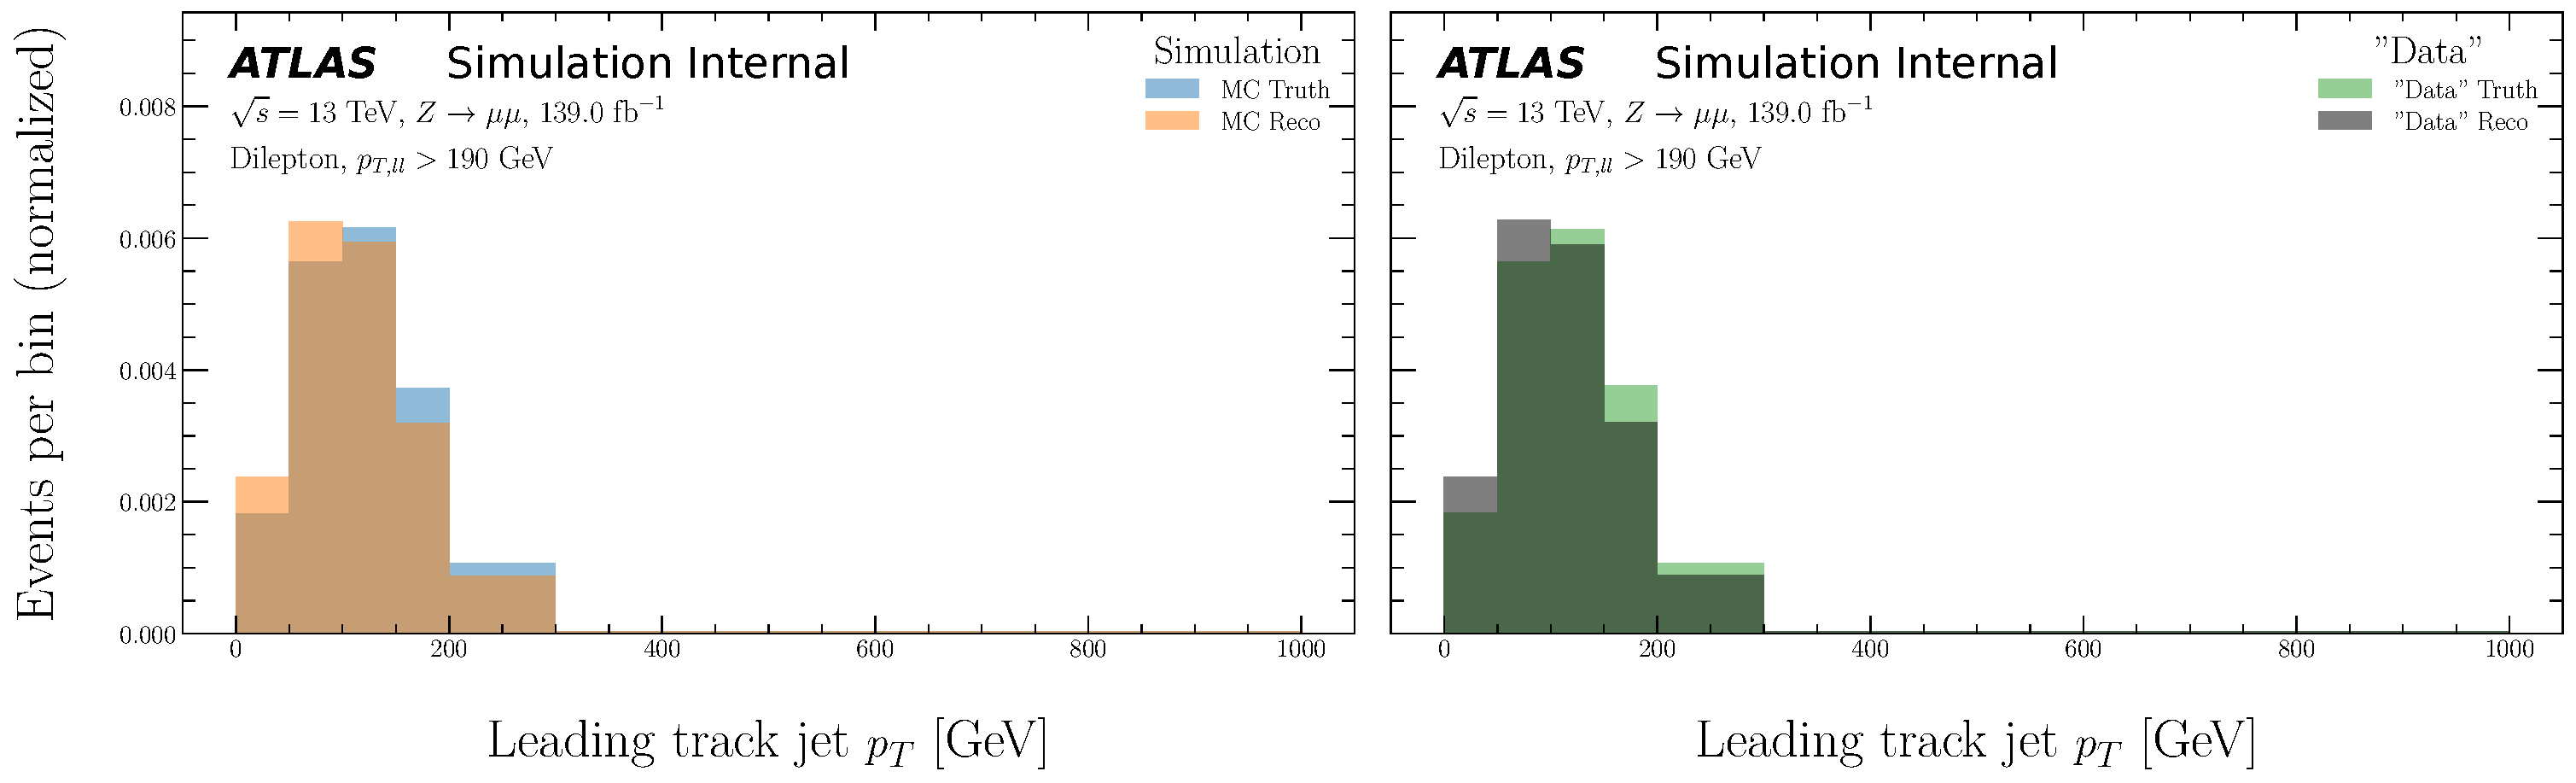
\includegraphics[width=0.95\textwidth]{figures/ATLASOmniFold-StressTest/ATLASOmniFold-TechnicalClosureTest/MultiFold/pT_trackj1/ATLASOmniFold-TechnicalClosureTest-MultiFold-pT_trackj1-Distributions.pdf}}\\
\subfloat[After 1 iteration]{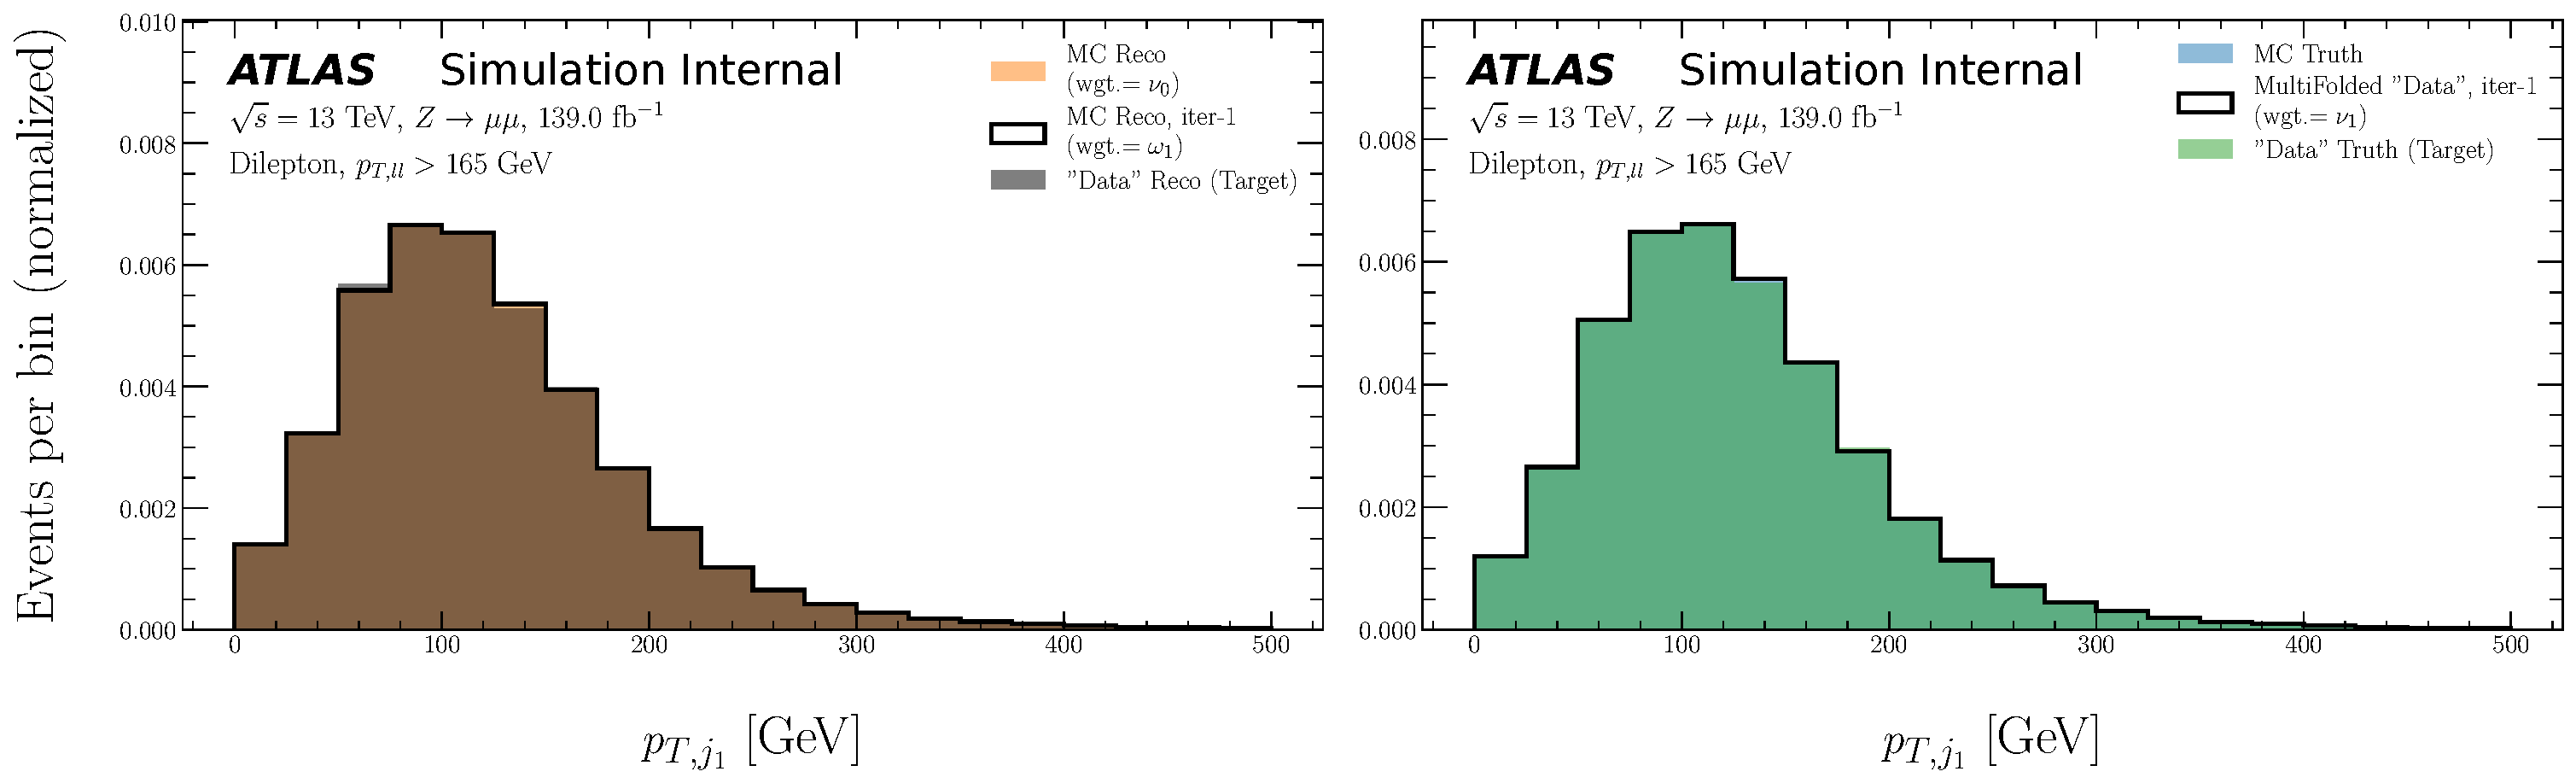
\includegraphics[width=0.95\textwidth]{figures/ATLASOmniFold-StressTest/ATLASOmniFold-TechnicalClosureTest/MultiFold/pT_trackj1/ATLASOmniFold-TechnicalClosureTest-MultiFold-pT_trackj1-Iteration01.pdf}}
\caption{A technical closure test for the $p_T$ of the leading track jet using MultiFold (16 observables are simultaneously unfolded).  The top plot show the input histograms and the bottom plots are the results after one iteration of OmniFold.  By construction the top left and top right histograms are statistically identical.}
\label{fig:technicalclosureMulti:pT_trackj1}
\end{figure}

\begin{figure}[h!]
\centering
\subfloat[Input histograms]{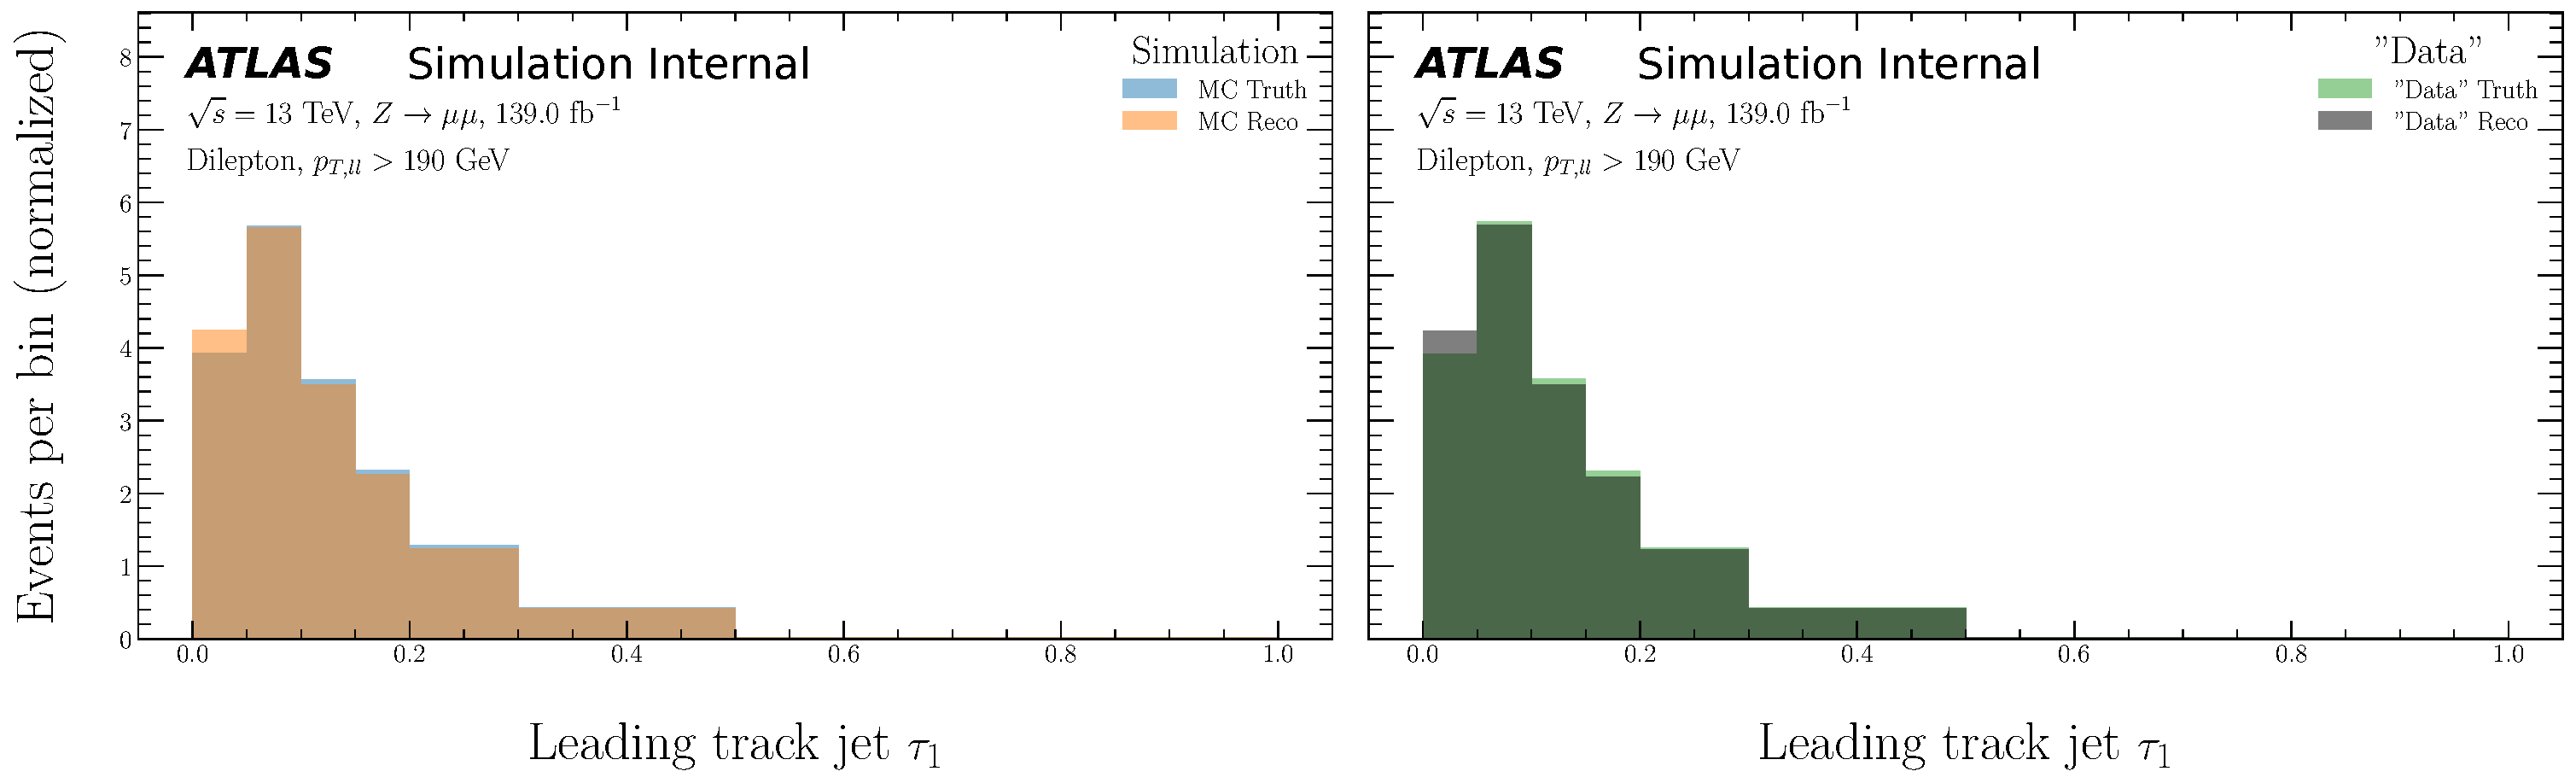
\includegraphics[width=0.89\textwidth]{figures/ATLASOmniFold-StressTest/ATLASOmniFold-TechnicalClosureTest/MultiFold/tau1_trackj1/ATLASOmniFold-TechnicalClosureTest-MultiFold-tau1_trackj1-Distributions.pdf}}\\
\subfloat[After 1 iteration]{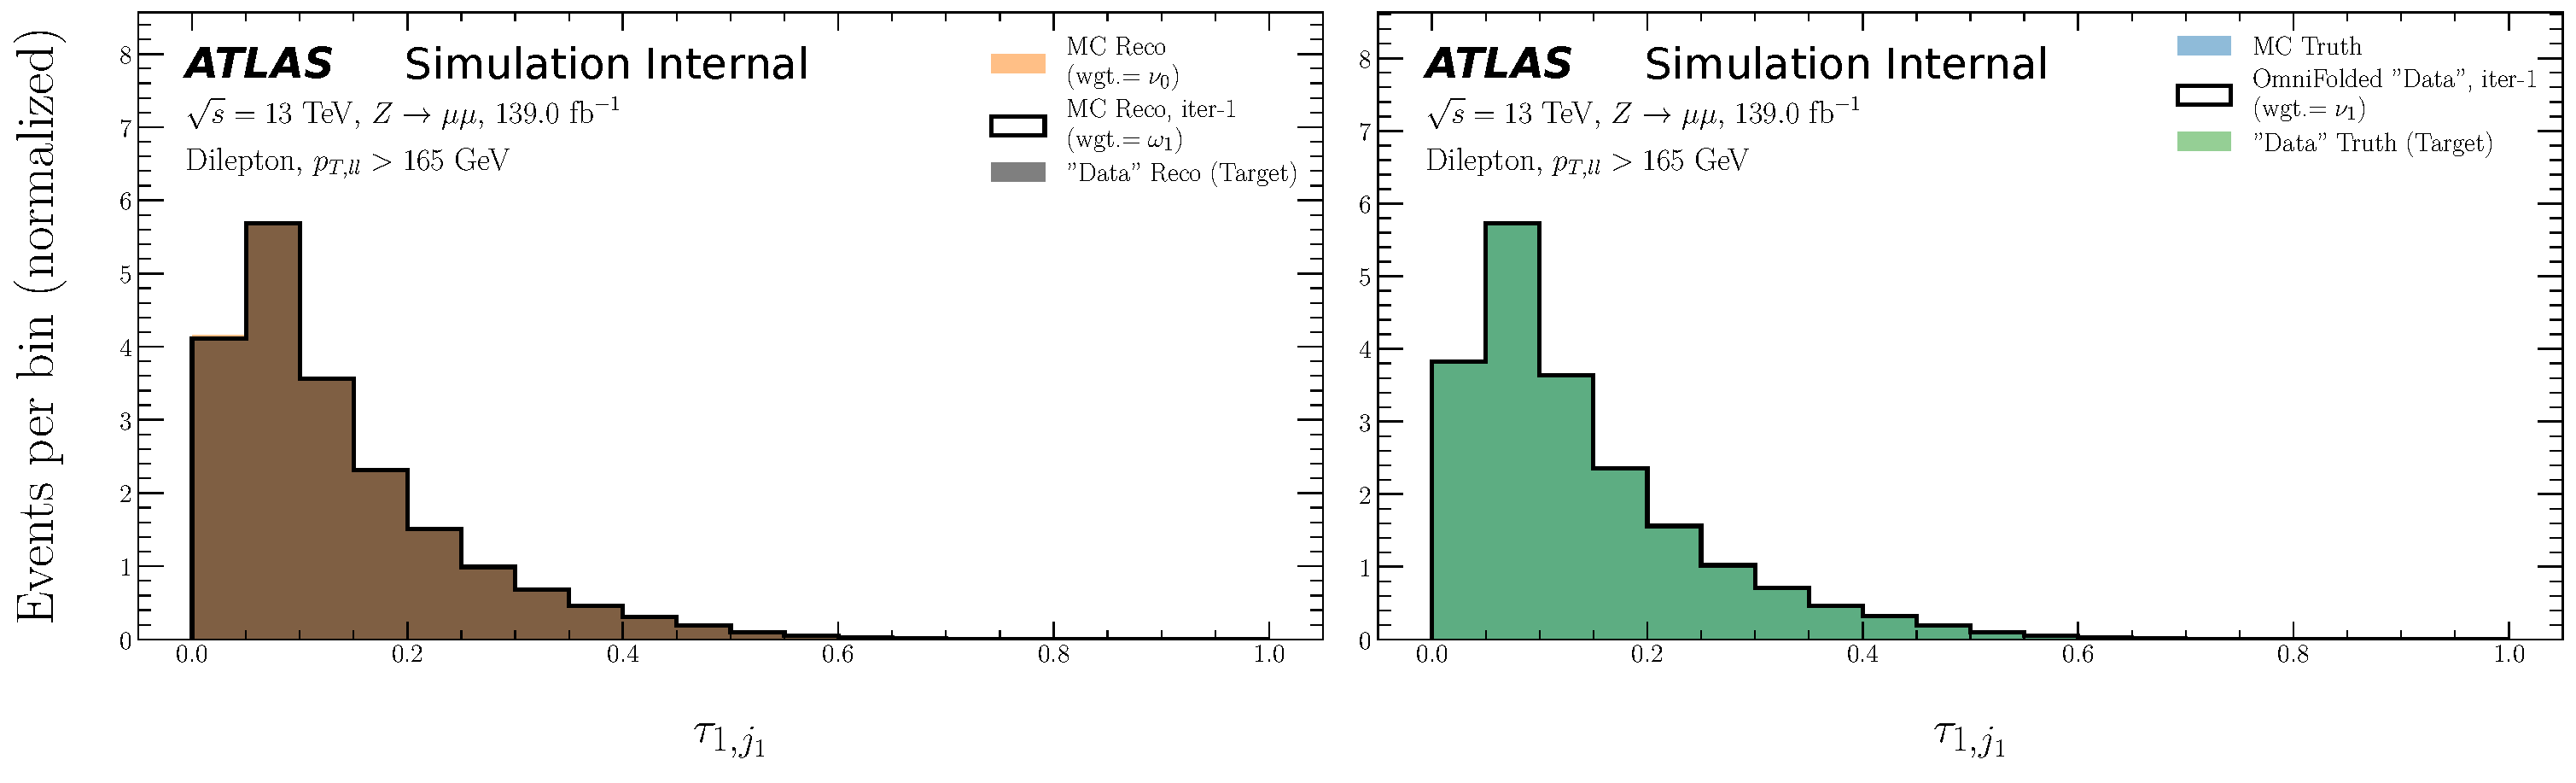
\includegraphics[width=0.95\textwidth]{figures/ATLASOmniFold-StressTest/ATLASOmniFold-TechnicalClosureTest/MultiFold/tau1_trackj1/ATLASOmniFold-TechnicalClosureTest-MultiFold-tau1_trackj1-Iteration01.pdf}}
\caption{A technical closure test for the $\tau_1$ of the leading track jet using MultiFold (16 observables are simultaneously unfolded).  The top plot show the input histograms and the bottom plots are the results after one iteration of OmniFold.  By construction the top left and top right histograms are statistically identical.}
\label{fig:technicalclosureMulti:tau1_trackj1}
\end{figure}

\begin{figure}[h!]
\centering
\subfloat[Input histograms]{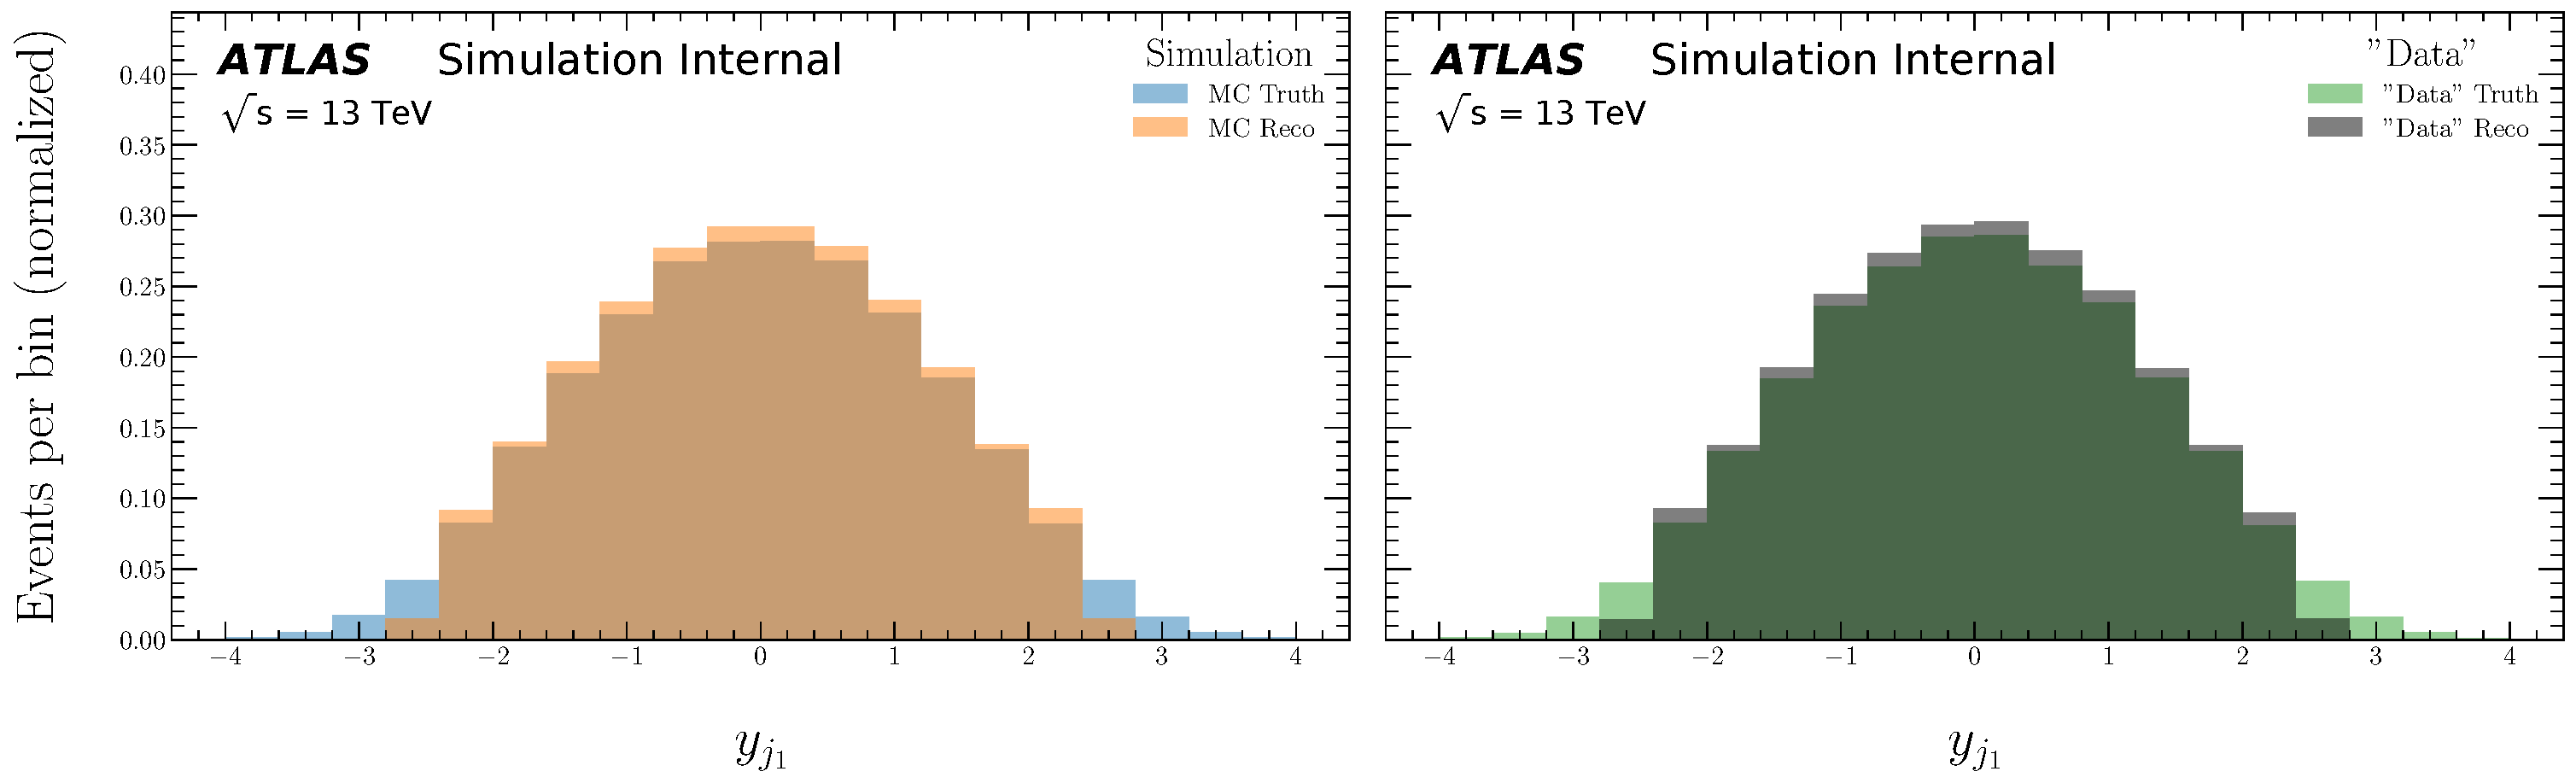
\includegraphics[width=0.95\textwidth]{figures/ATLASOmniFold-StressTest/ATLASOmniFold-TechnicalClosureTest/MultiFold/y_trackj1/ATLASOmniFold-TechnicalClosureTest-MultiFold-y_trackj1-Distributions.pdf}}\\
\subfloat[After 1 iteration]{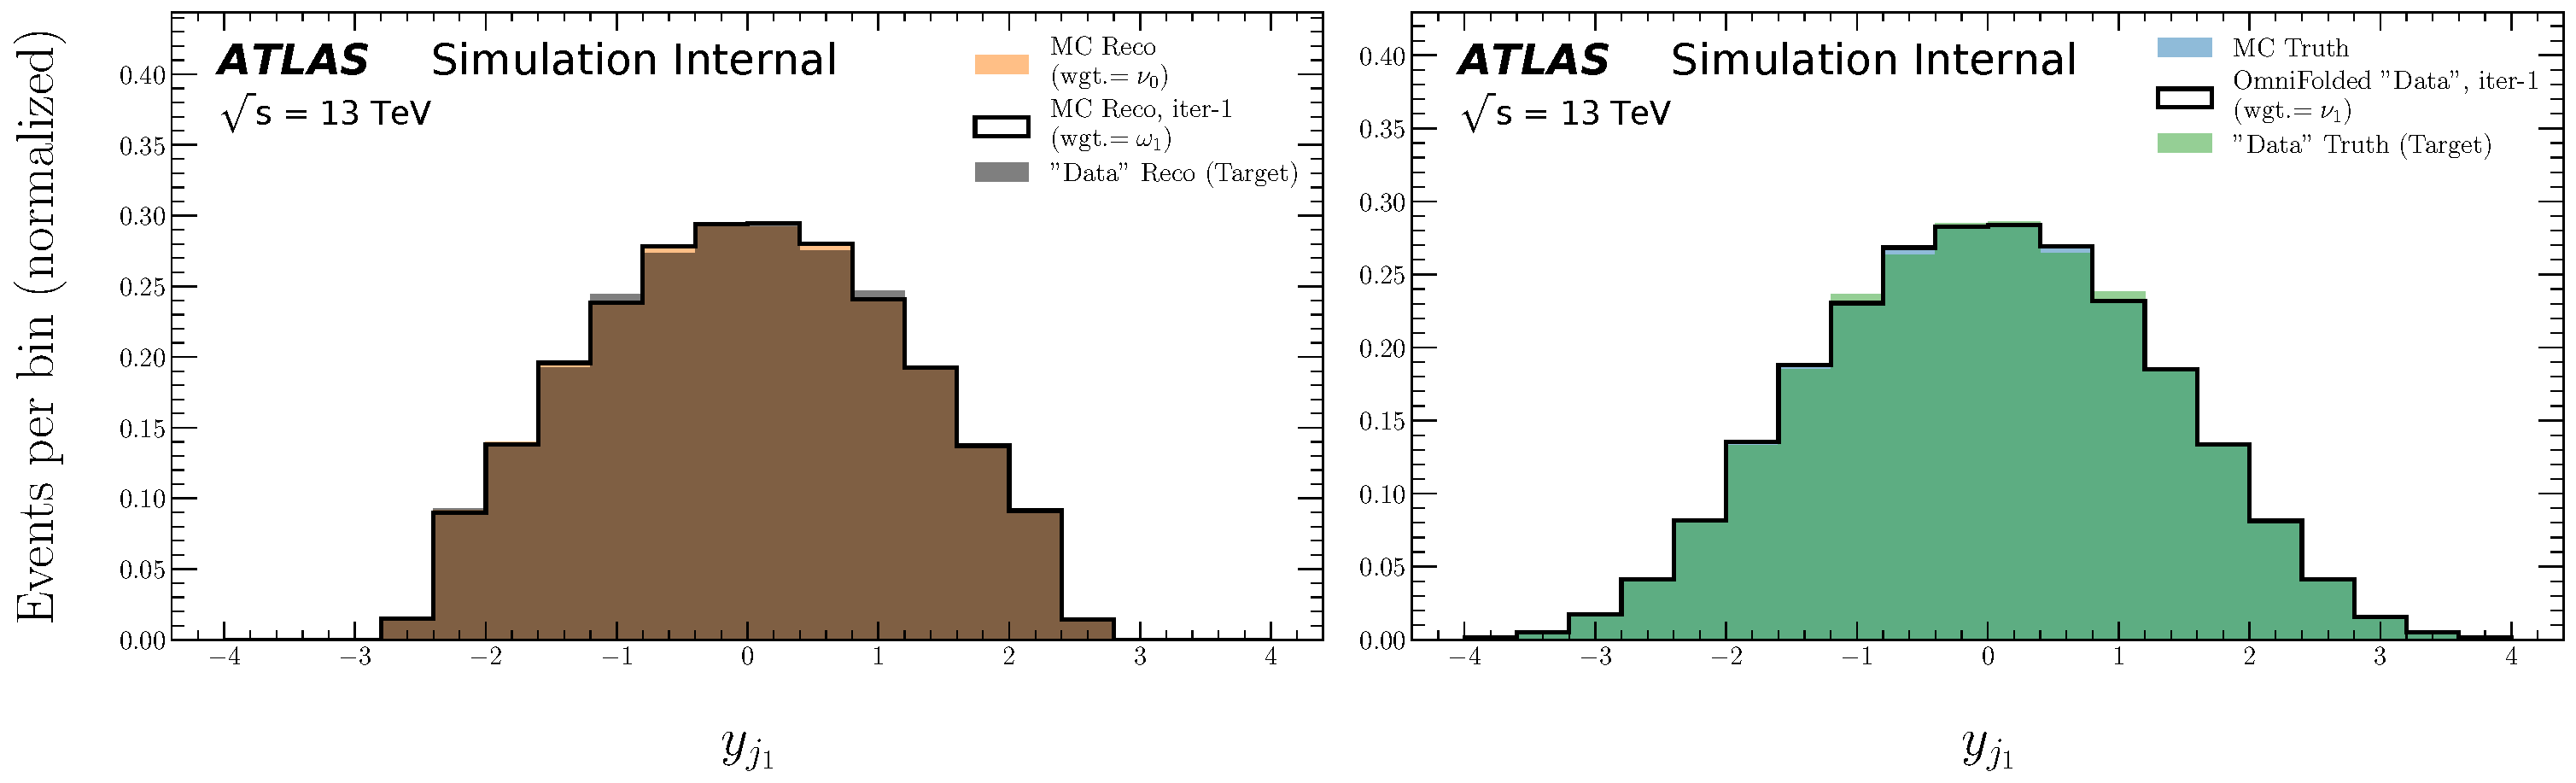
\includegraphics[width=0.95\textwidth]{figures/ATLASOmniFold-StressTest/ATLASOmniFold-TechnicalClosureTest/MultiFold/y_trackj1/ATLASOmniFold-TechnicalClosureTest-MultiFold-y_trackj1-Iteration01.pdf}}
\caption{A technical closure test for the rapidity of the leading track jet using MultiFold (16 observables are simultaneously unfolded).  The top plot show the input histograms and the bottom plots are the results after one iteration of OmniFold.  By construction the top left and top right histograms are statistically identical.}
\label{fig:technicalclosureMulti:y_trackj1}
\end{figure}

\subsection{Artificial Stress Tests}
\label{sec:technicalclosure2}

In this section, we apply artificial weights to the events in order to shift the various distributions and we show that we can recover the unshifted distributions.  In particular, we divide the Pythia sample in half again and apply stress weights to the half labeled `simulation'.  In one case (Sec.~\ref{sec:stress:deterministic}), these weights are a deterministic function of the input features.  In a second case (Sec.~\ref{sec:stress:stochastic}), the weights are stochastic function of the inputs.

\clearpage

\subsubsection{Deterministic Weights}
\label{sec:stress:deterministic}

For a given event $x$ in sample $X$, the stress weights are given by

\begin{align}
\label{eq:stressweights}
w = w_{MC}\,(-\min_{x'\in X}\mathcal{Z}(x')+\mathcal{Z}(x))^n\,,
\end{align}
%
where $w_{MC}$ is the Monte Carlo event weight and $\mathcal{Z}$ gives the Z-score of $x\in X$. We do a basic weight standardization given all stress weights $W$ by doing $w\mapsto\frac{w}{\langle W\rangle}$. These stress weights are constructed to induce a right shift in the given distribution. Note that a larger value of $n$ induces a more intense right-shift in the stressed distributions.  For the UniFold distributions, a value of $n=2$ is used; for the MultiFold distributions, we use $n=3$.

\paragraph{UniFold}

Figures~\ref{fig:stressa_mass} and~\ref{fig:stressa_Ntracks_trackj1} are examples for the leading track jet mass and the number of tracks inside jets.  Additional examples can be found in App~\ref{sec:stressunifolddet}.

\begin{figure}[h!]
\centering
\subfloat[Weights]{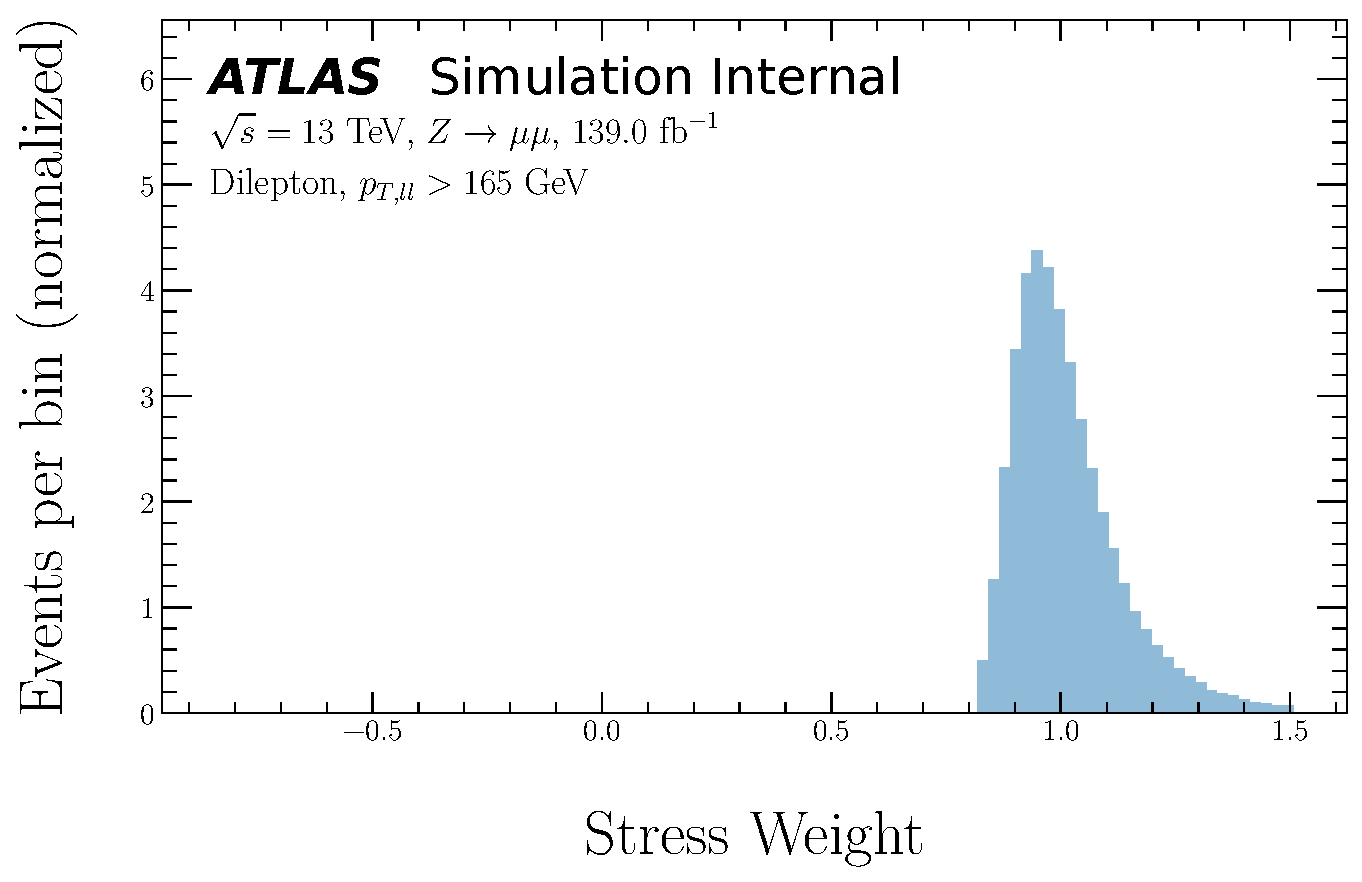
\includegraphics[width=0.45\textwidth]{figures/ATLASOmniFold-StressTest/ATLASOmniFold-StressTestA/UniFold/m_trackj1/ATLASOmniFold-StressTestA-UniFold-m_trackj1-StressWeightsHist.pdf}}\\
\subfloat[Input histograms]{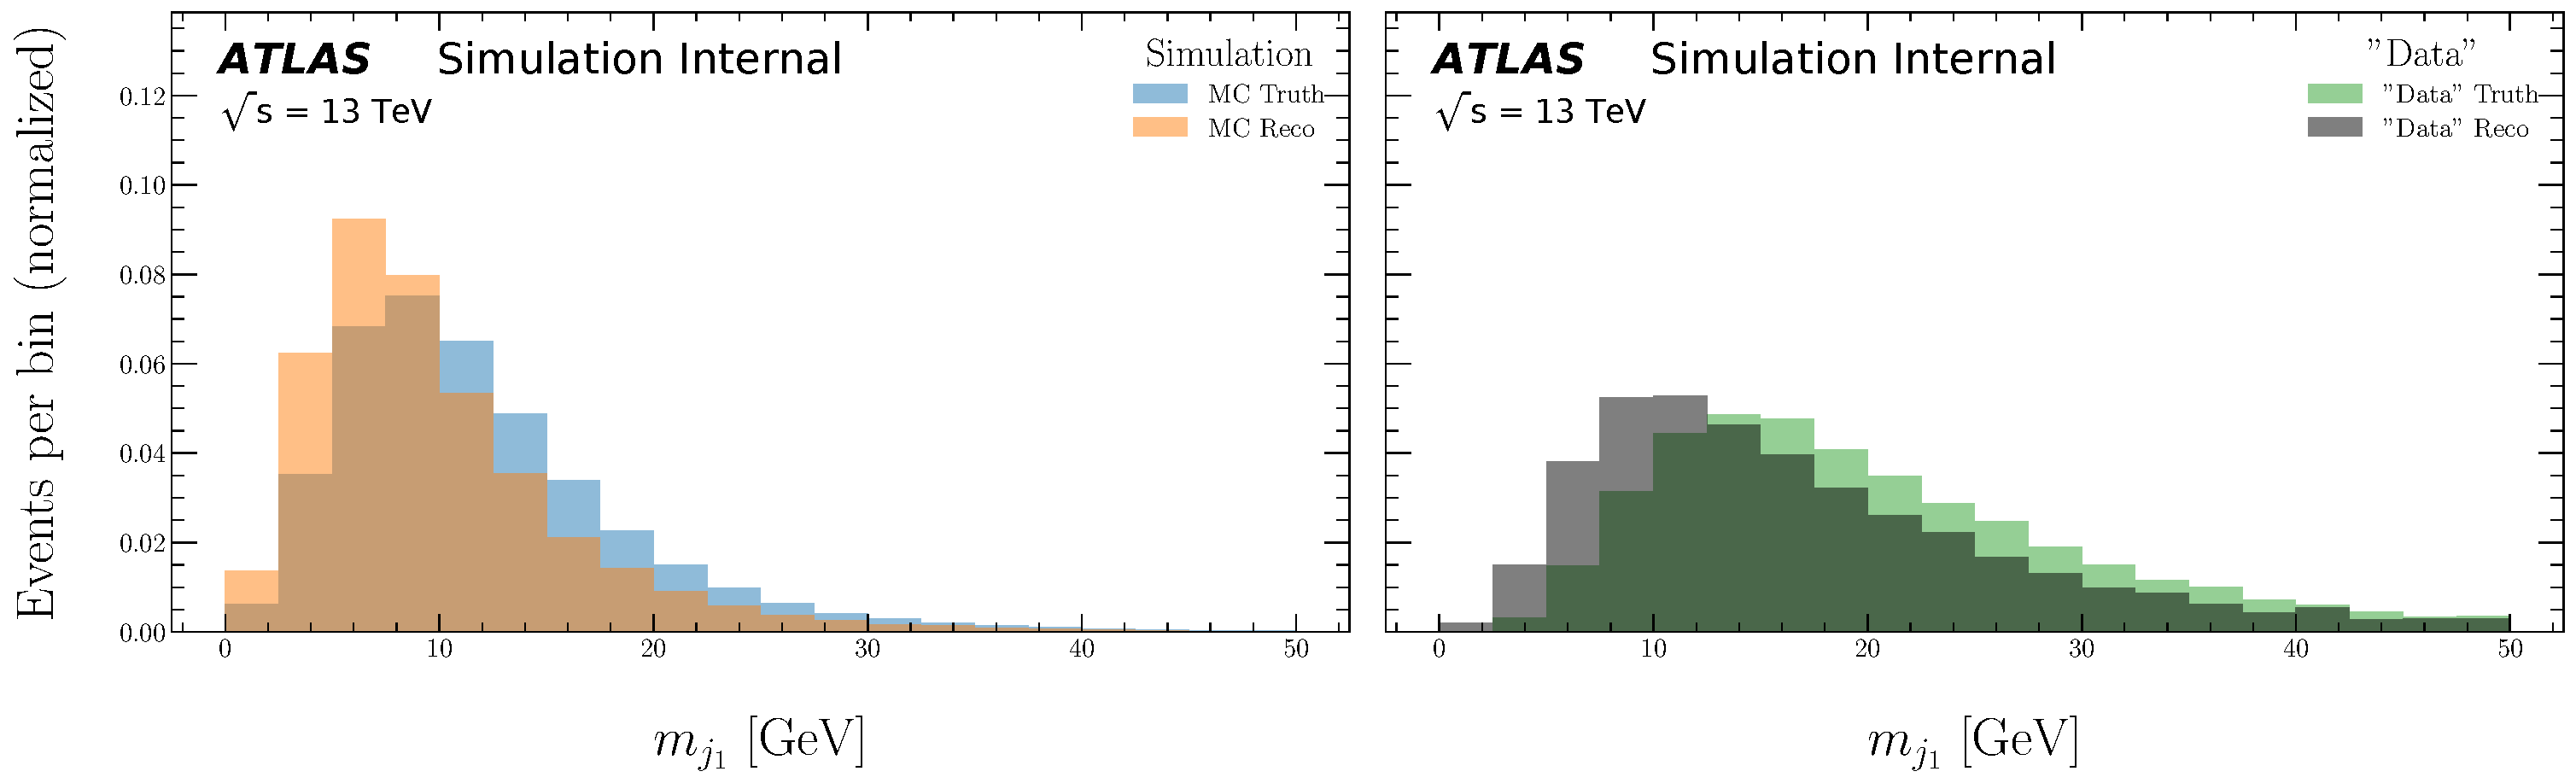
\includegraphics[width=0.85\textwidth]{figures/ATLASOmniFold-StressTest/ATLASOmniFold-StressTestA/UniFold/m_trackj1/ATLASOmniFold-StressTestA-UniFold-m_trackj1-Distributions}}\\
\subfloat[After 1 iteration]{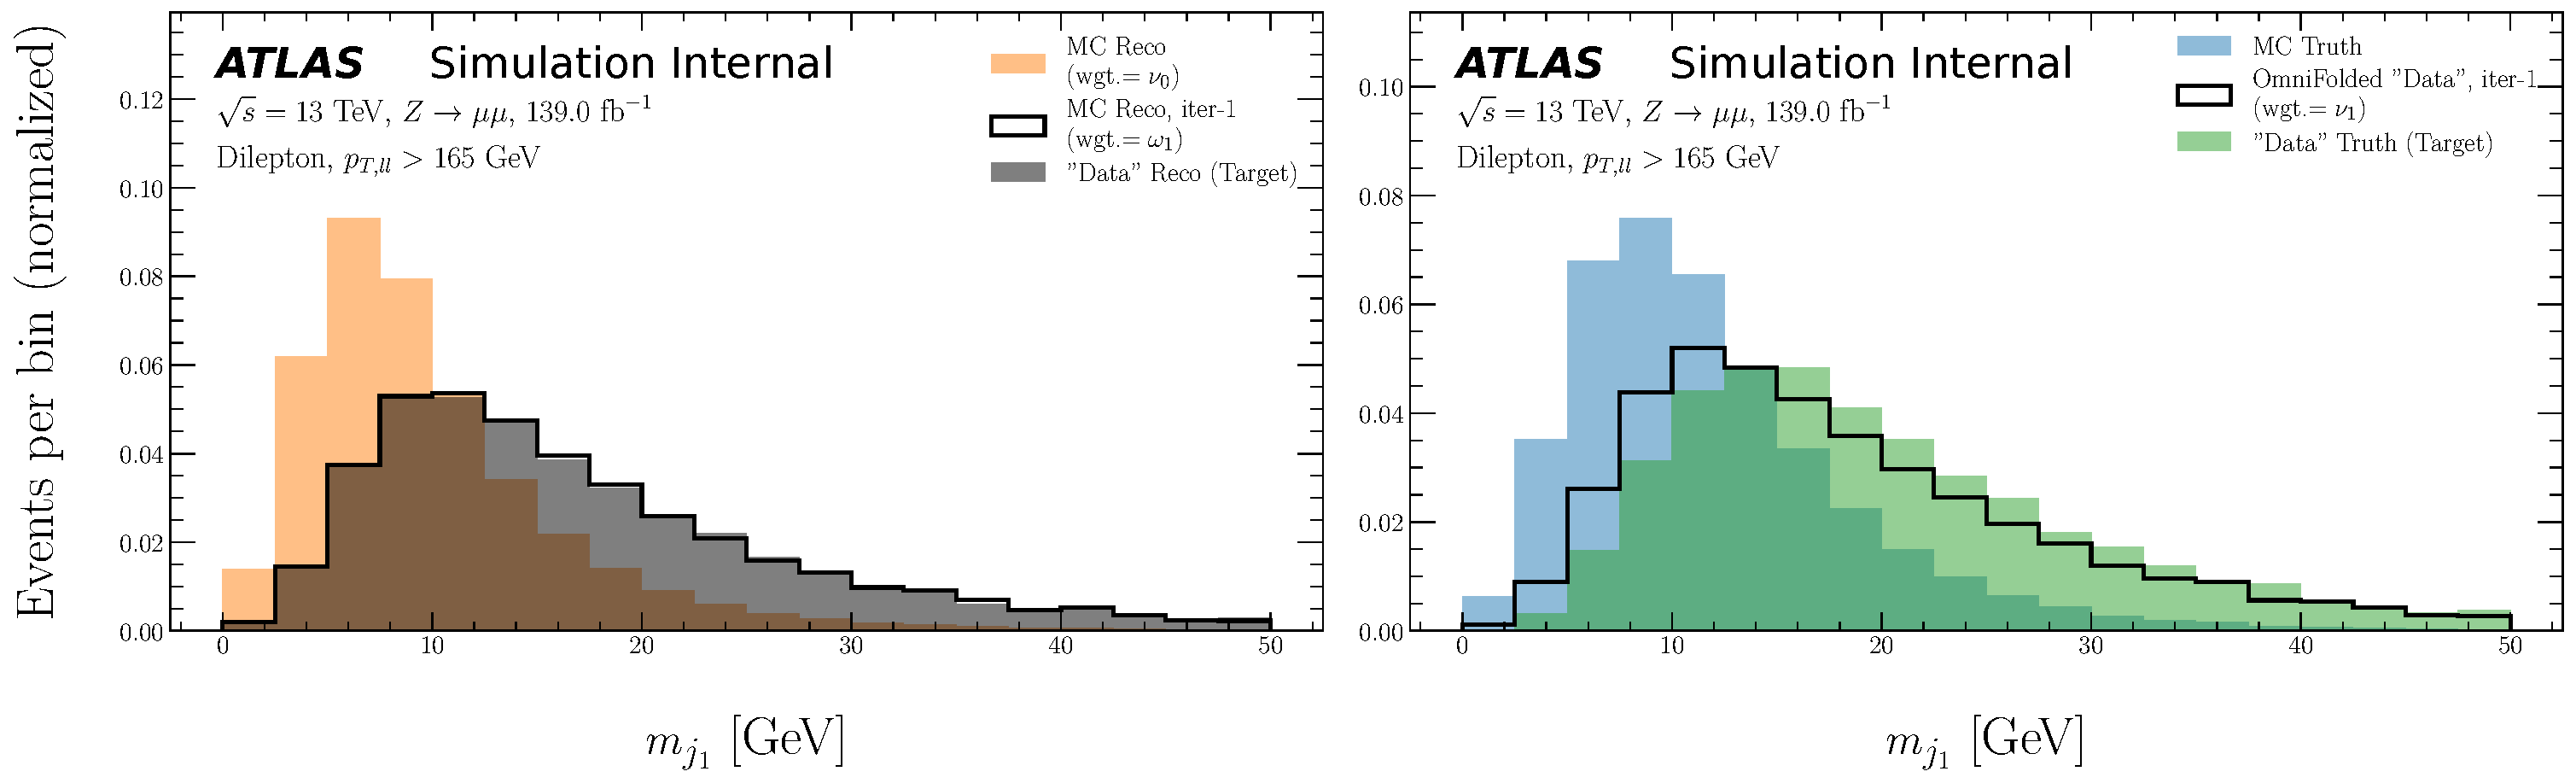
\includegraphics[width=0.85\textwidth]{figures/ATLASOmniFold-StressTest/ATLASOmniFold-StressTestA/UniFold/m_trackj1/ATLASOmniFold-StressTestA-UniFold-m_trackj1-Iteration01}}\\
\subfloat[After 2 iterations]{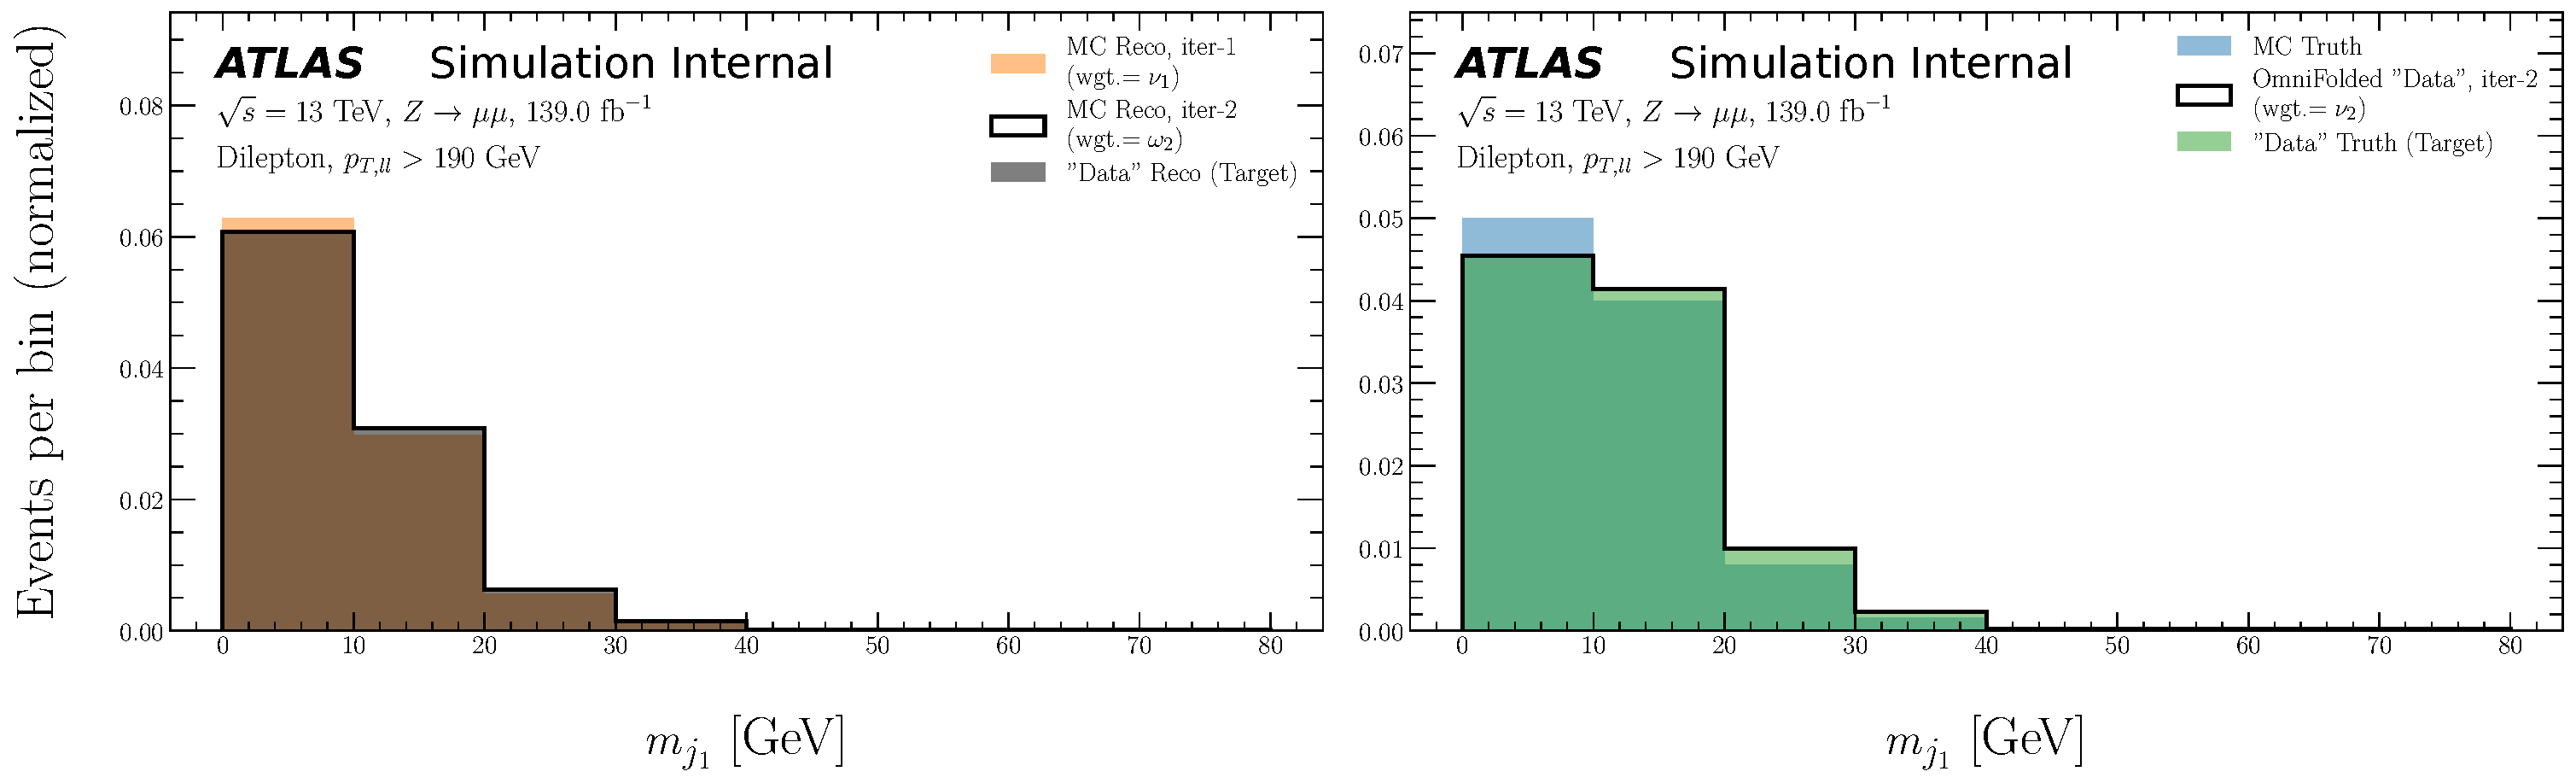
\includegraphics[width=0.85\textwidth]{figures/ATLASOmniFold-StressTest/ATLASOmniFold-StressTestA/UniFold/m_trackj1/ATLASOmniFold-StressTestA-UniFold-m_trackj1-Iteration02}}
\phantomcaption
\end{figure}

\begin{figure}[h!]
\centering
\ContinuedFloat
\subfloat[After 3 iterations]{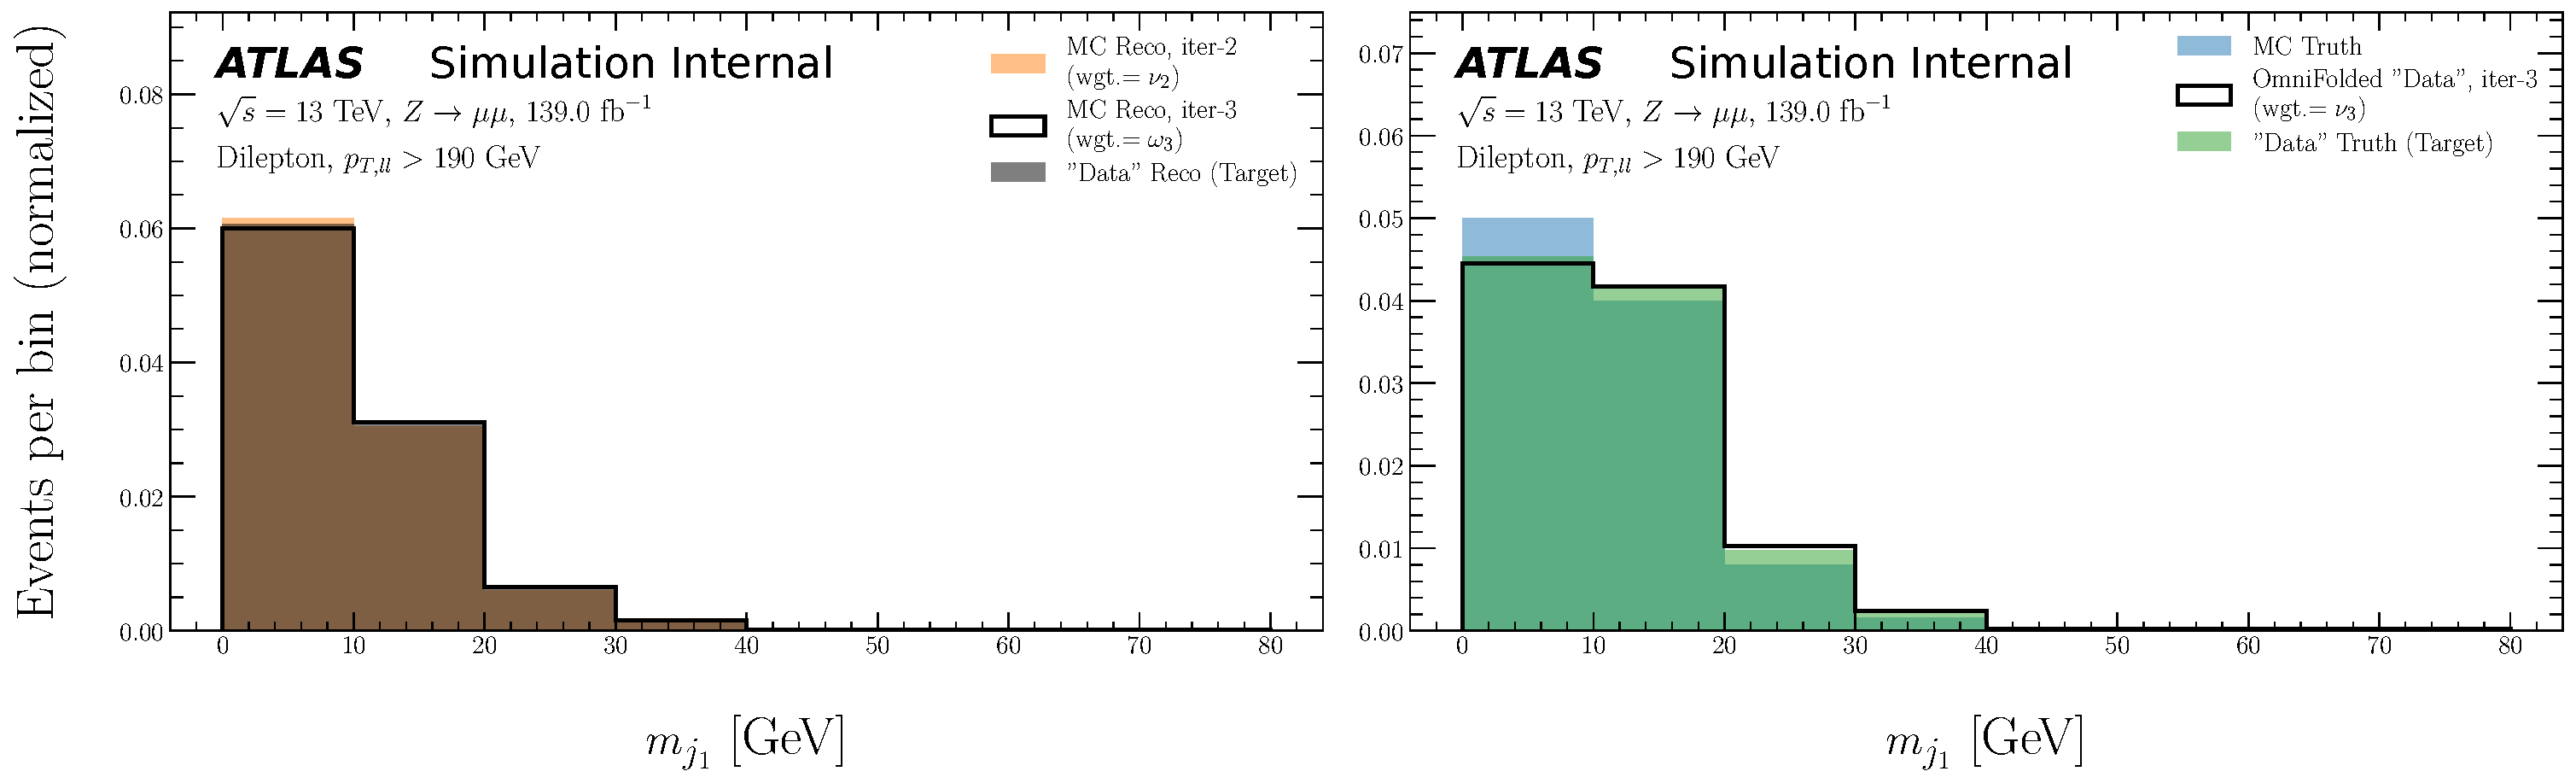
\includegraphics[width=0.85\textwidth]{figures/ATLASOmniFold-StressTest/ATLASOmniFold-StressTestA/UniFold/m_trackj1/ATLASOmniFold-StressTestA-UniFold-m_trackj1-Iteration03}}\\
\subfloat[After 4 iterations]{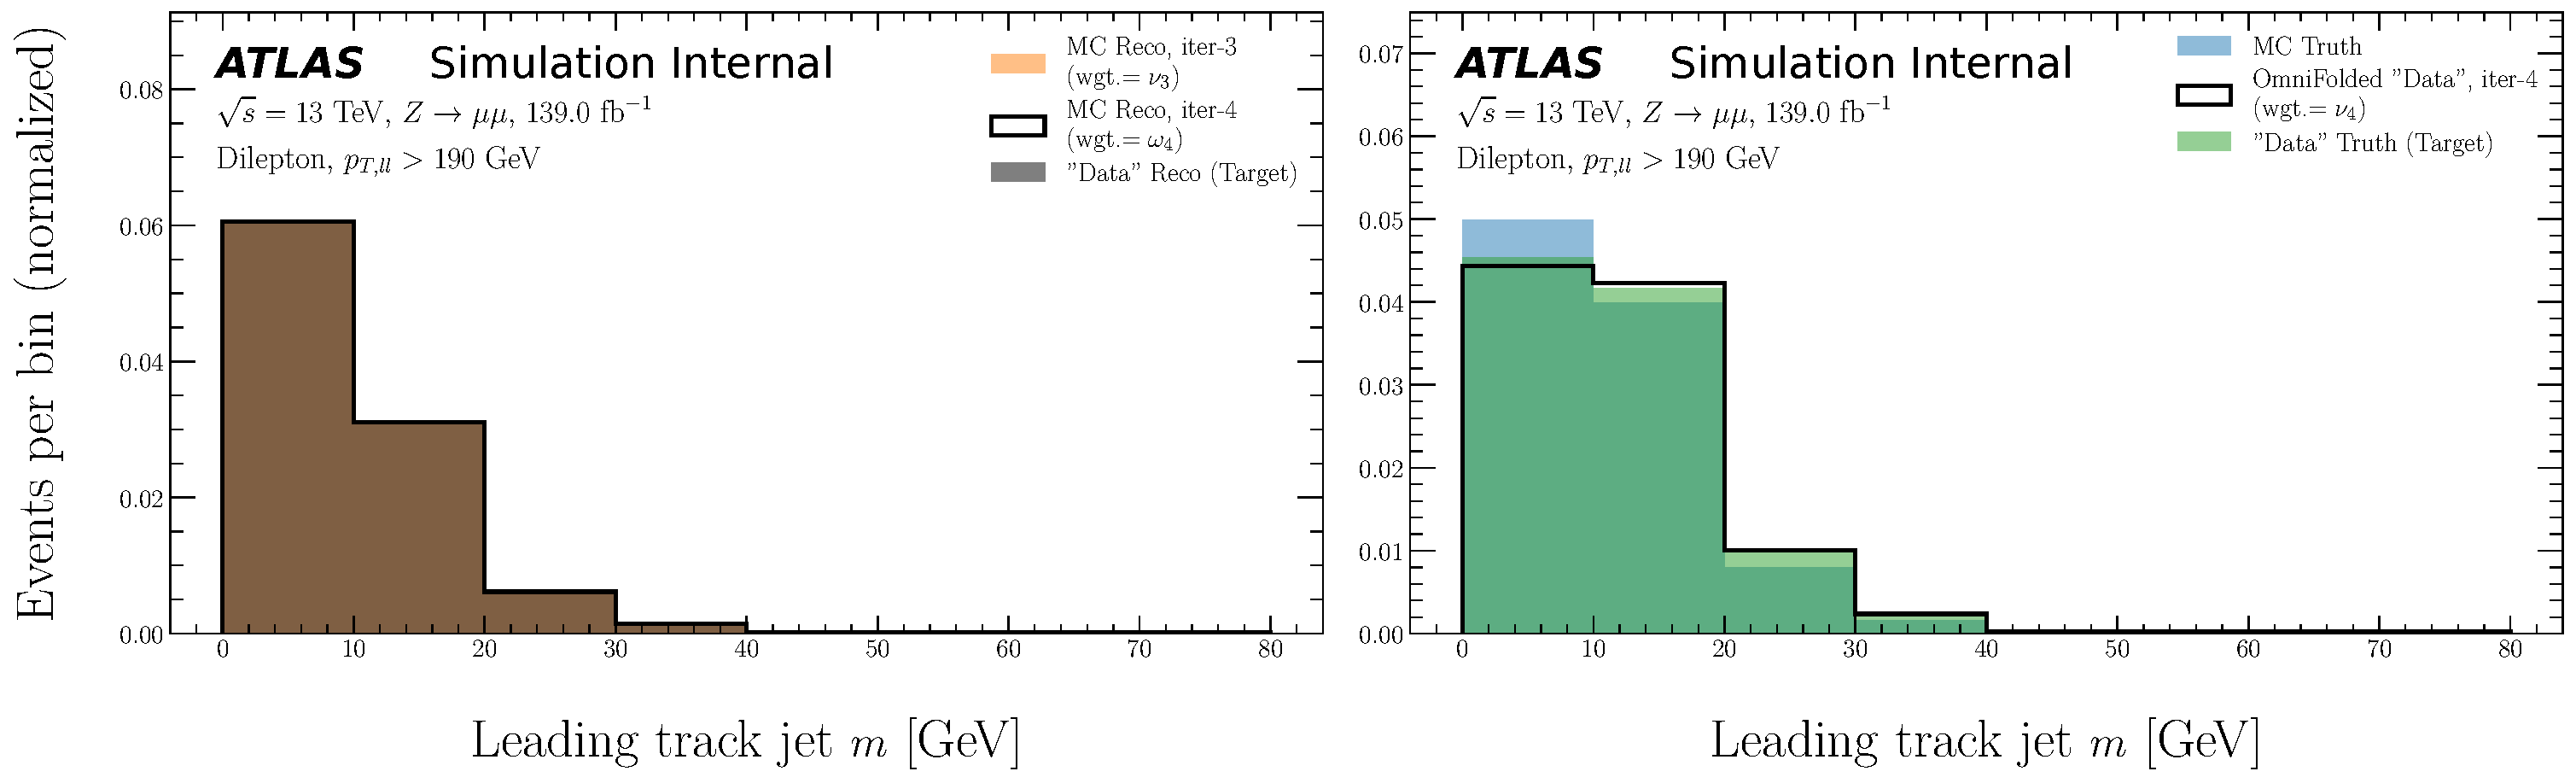
\includegraphics[width=0.85\textwidth]{figures/ATLASOmniFold-StressTest/ATLASOmniFold-StressTestA/UniFold/m_trackj1/ATLASOmniFold-StressTestA-UniFold-m_trackj1-Iteration04}}\\
\subfloat[After 5 iterations]{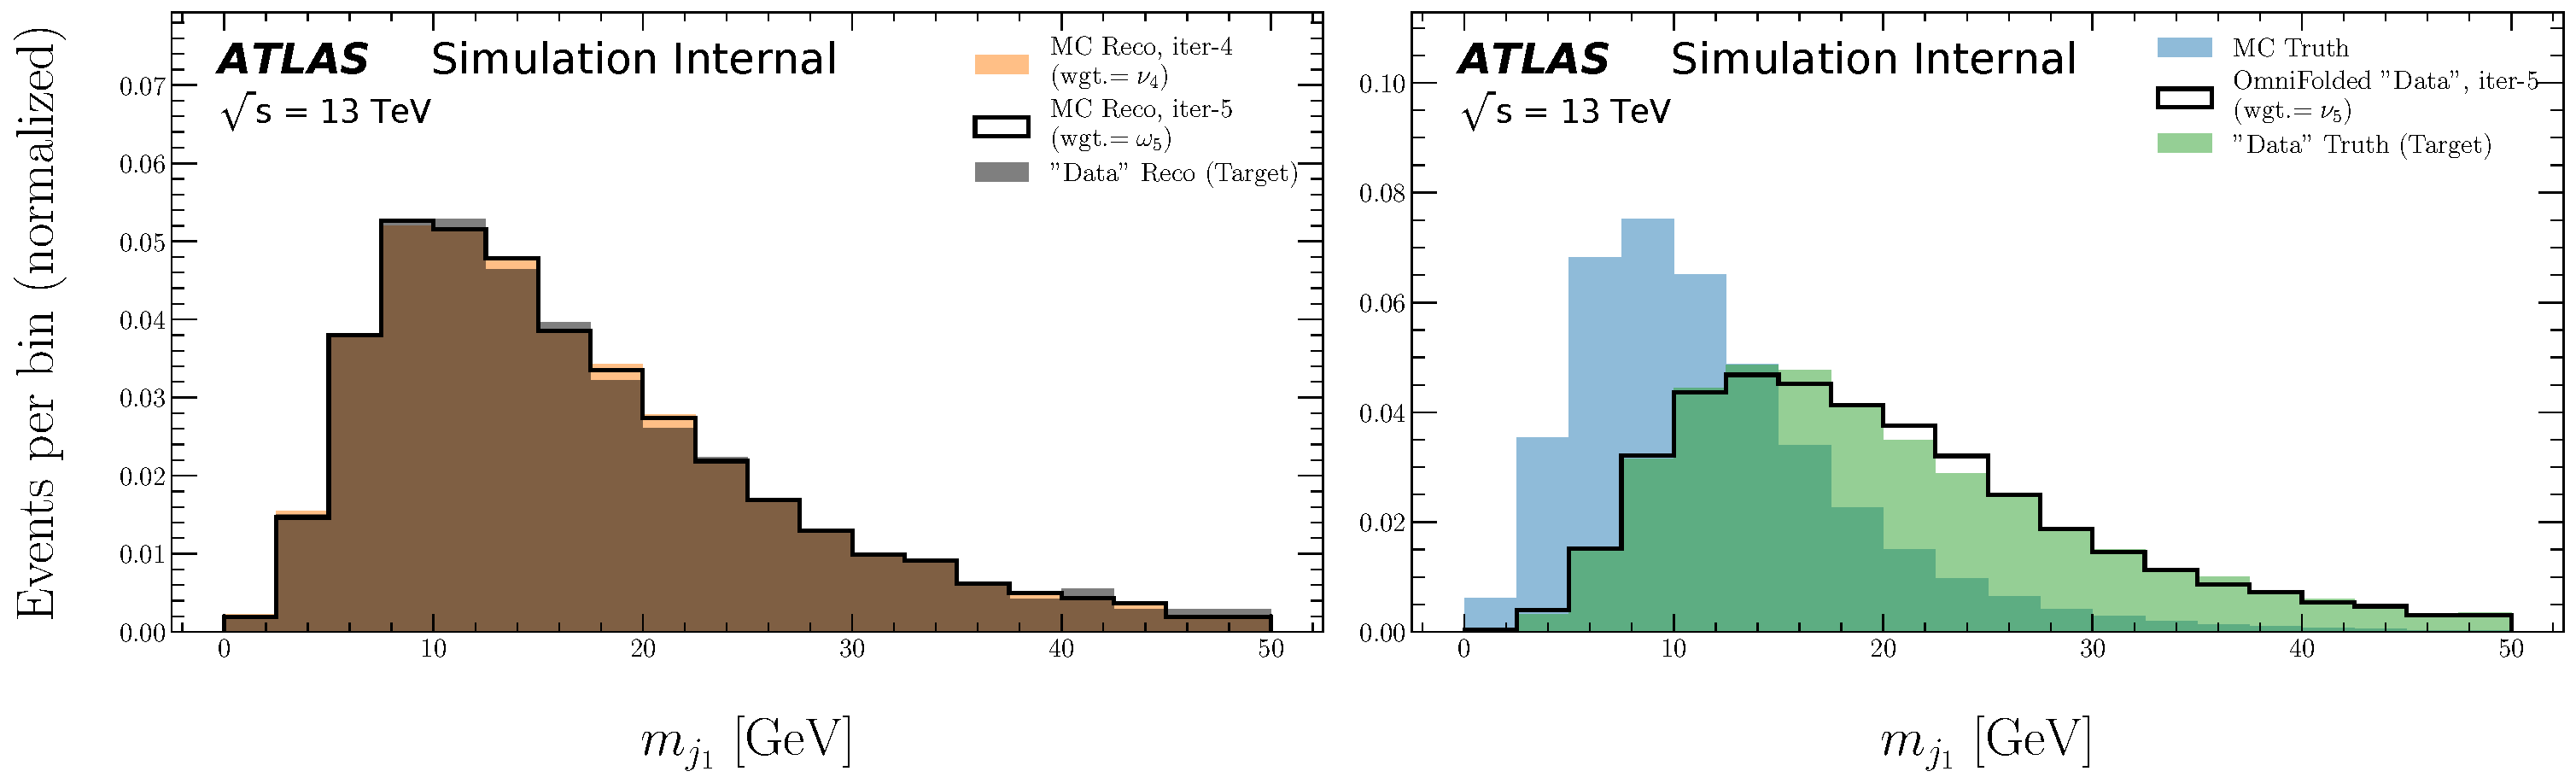
\includegraphics[width=0.85\textwidth]{figures/ATLASOmniFold-StressTest/ATLASOmniFold-StressTestA/UniFold/m_trackj1/ATLASOmniFold-StressTestA-UniFold-m_trackj1-Iteration05}}\\
\subfloat[After 6 iterations]{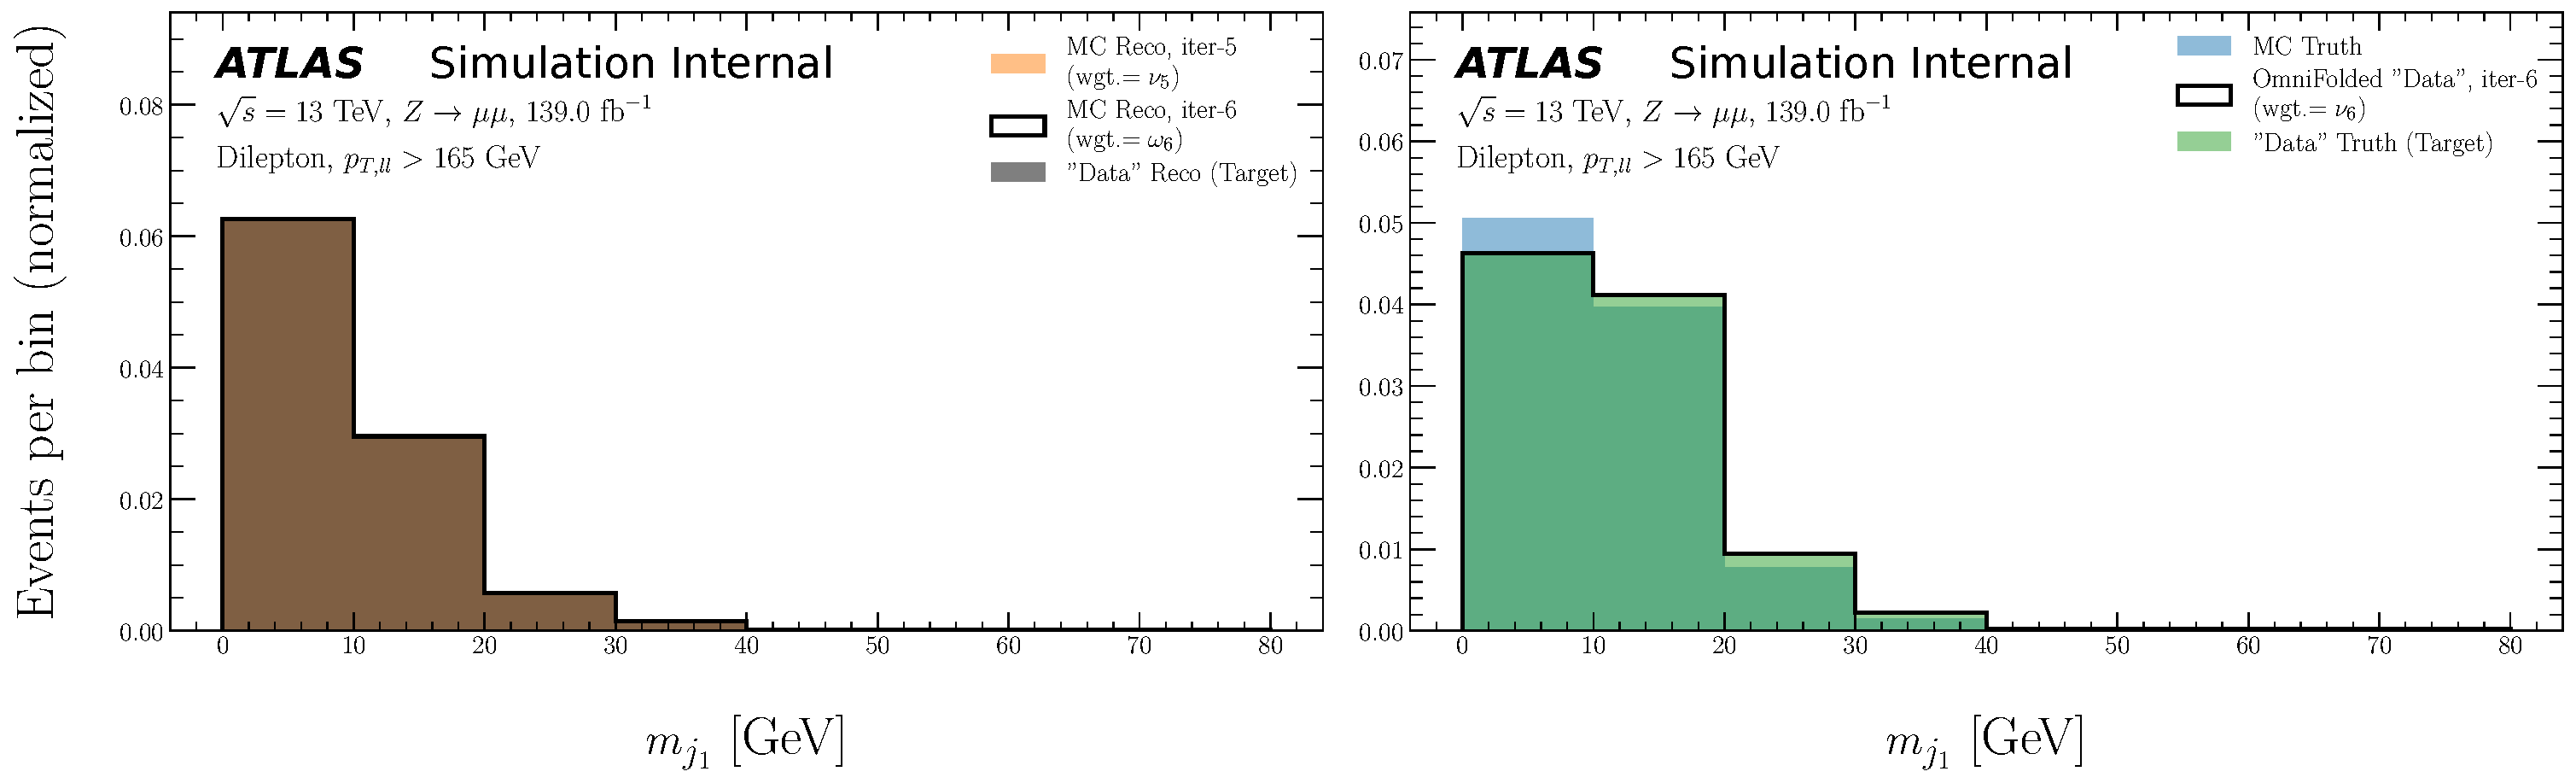
\includegraphics[width=0.85\textwidth]{figures/ATLASOmniFold-StressTest/ATLASOmniFold-StressTestA/UniFold/m_trackj1/ATLASOmniFold-StressTestA-UniFold-m_trackj1-Iteration06}}
\caption{A stress test for UniFold applied to the leading track jet mass.}
\label{fig:stressa_mass}
\end{figure}

\begin{figure}[h!]
\centering
\subfloat[Weights]{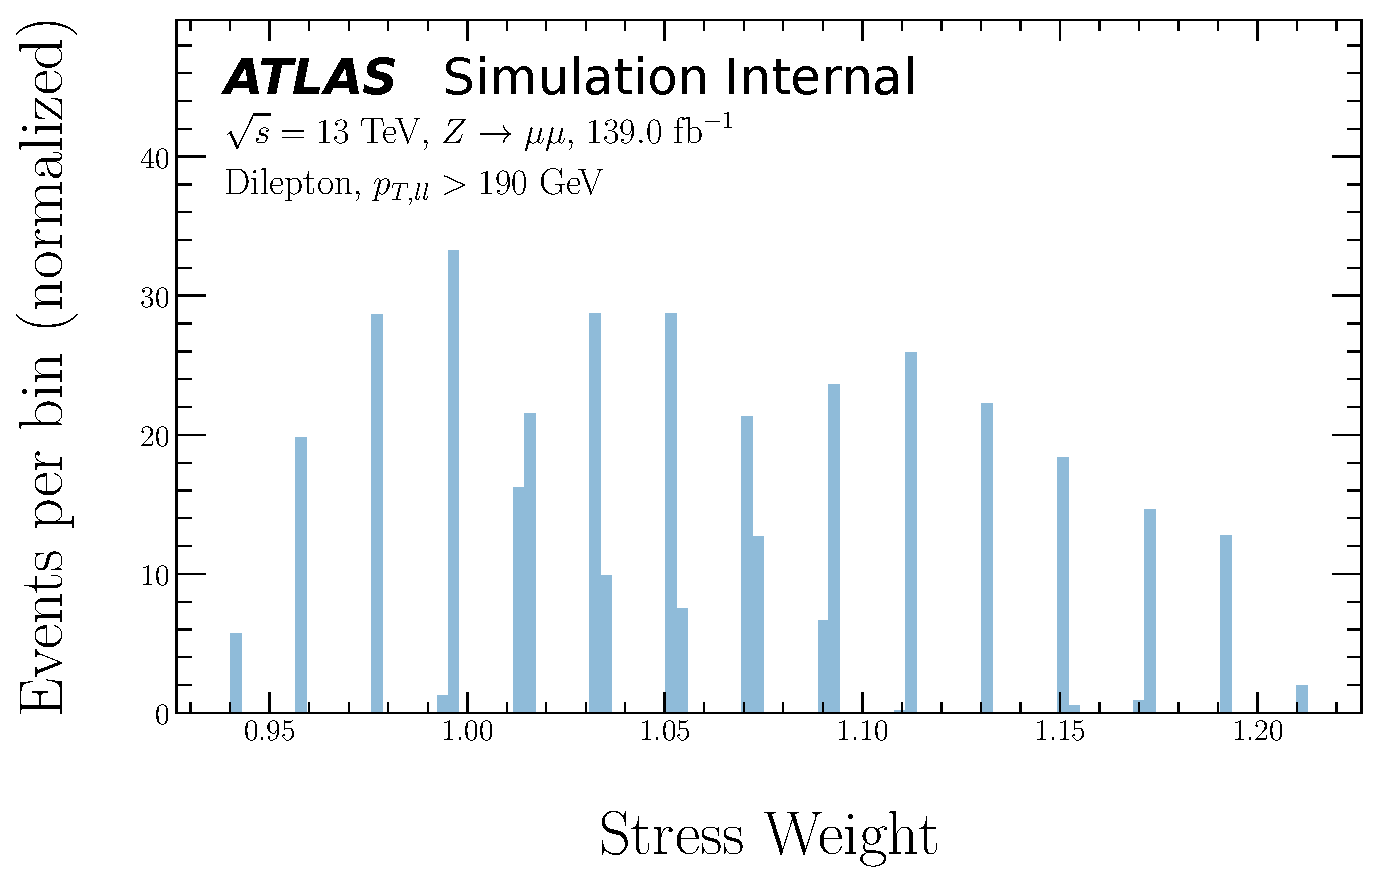
\includegraphics[width=0.45\textwidth]{figures/ATLASOmniFold-StressTest/ATLASOmniFold-StressTestA/UniFold/Ntracks_trackj1/ATLASOmniFold-StressTestA-UniFold-Ntracks_trackj1-StressWeightsHist.pdf}}\\
\subfloat[Input histograms]{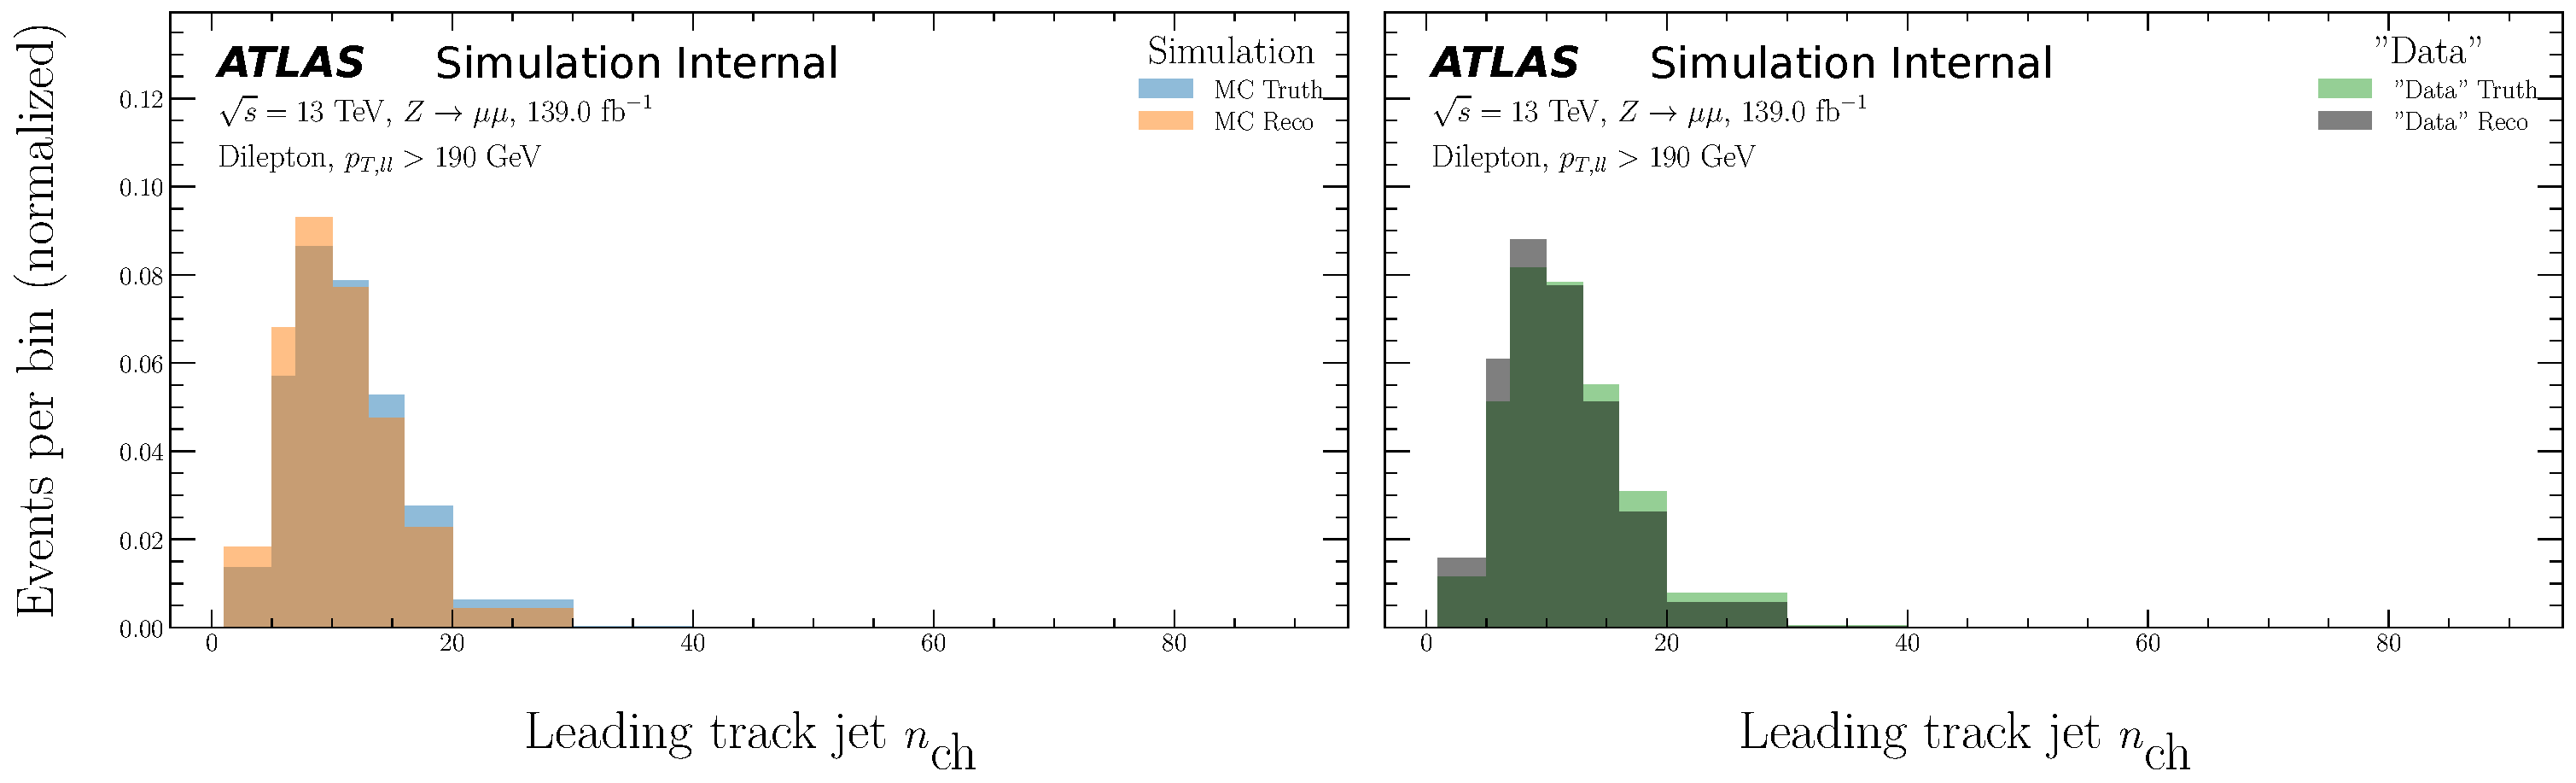
\includegraphics[width=0.85\textwidth]{figures/ATLASOmniFold-StressTest/ATLASOmniFold-StressTestA/UniFold/Ntracks_trackj1/ATLASOmniFold-StressTestA-UniFold-Ntracks_trackj1-Distributions}}\\
\subfloat[After 1 iteration]{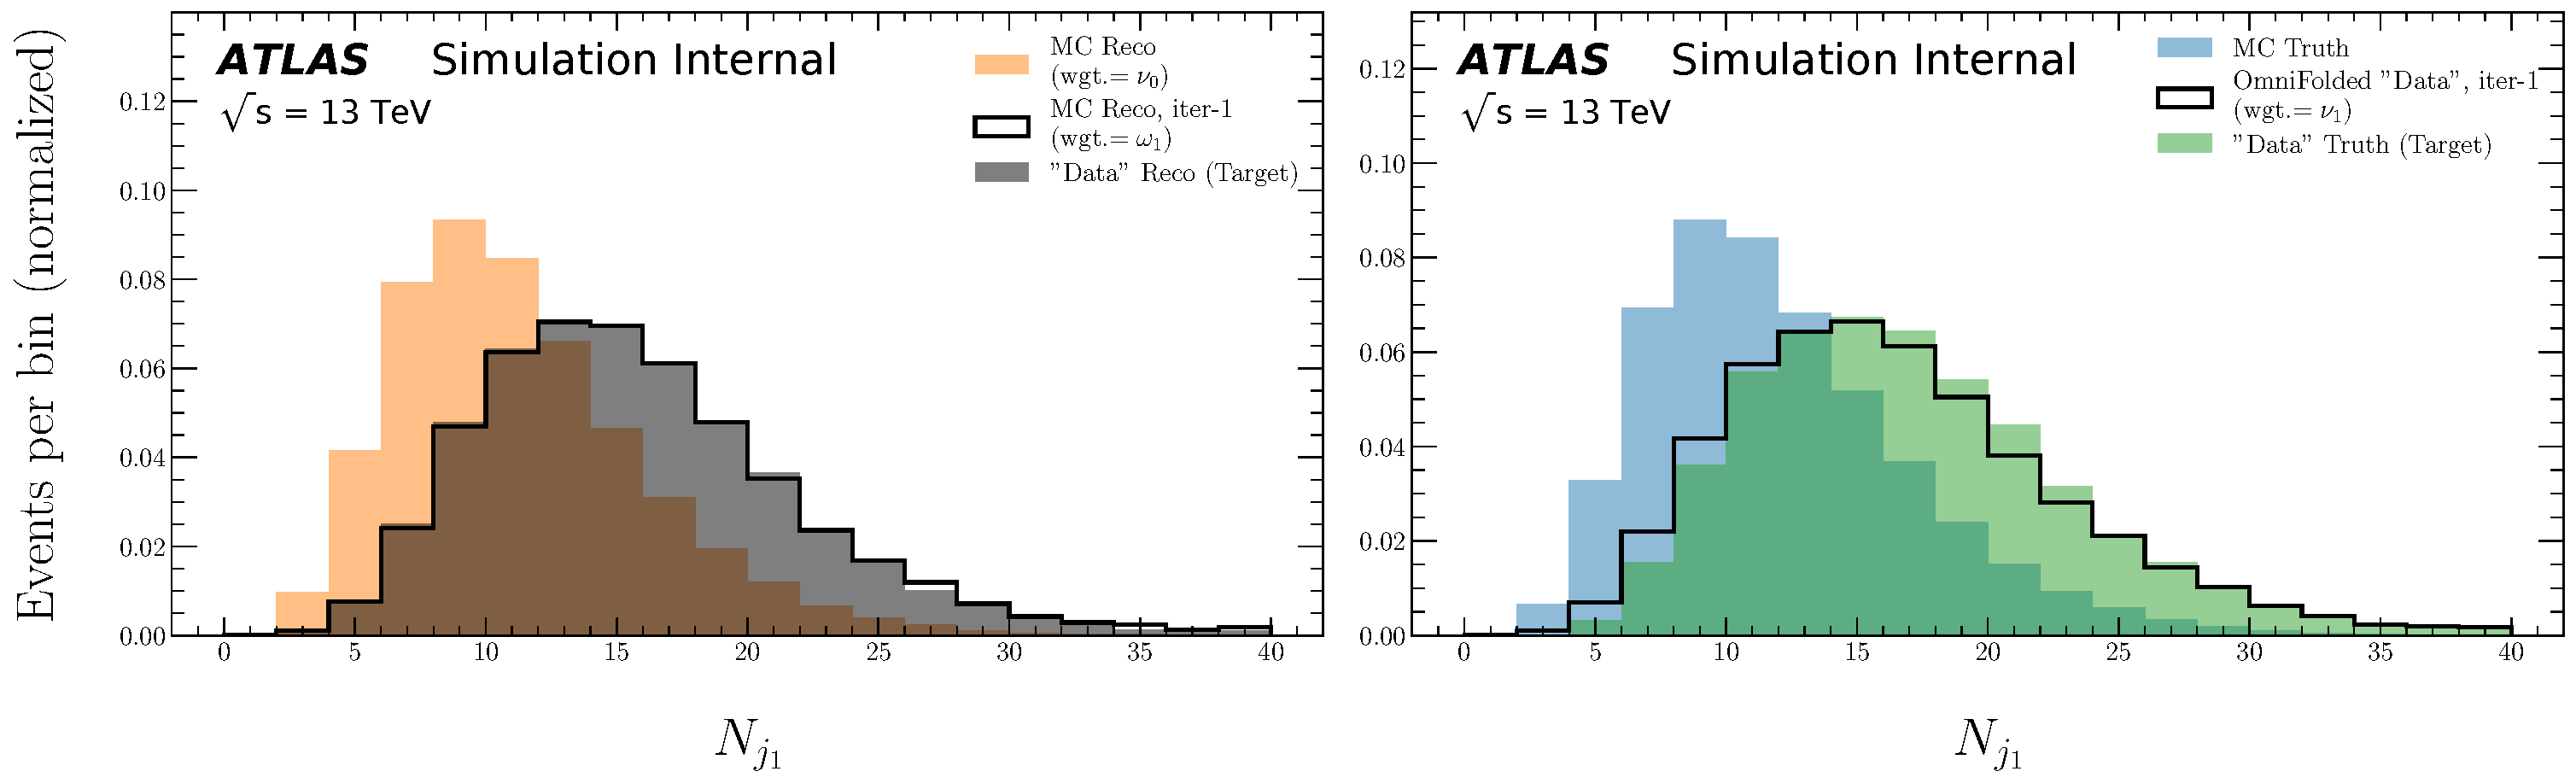
\includegraphics[width=0.85\textwidth]{figures/ATLASOmniFold-StressTest/ATLASOmniFold-StressTestA/UniFold/Ntracks_trackj1/ATLASOmniFold-StressTestA-UniFold-Ntracks_trackj1-Iteration01}}\\
\subfloat[After 2 iterations]{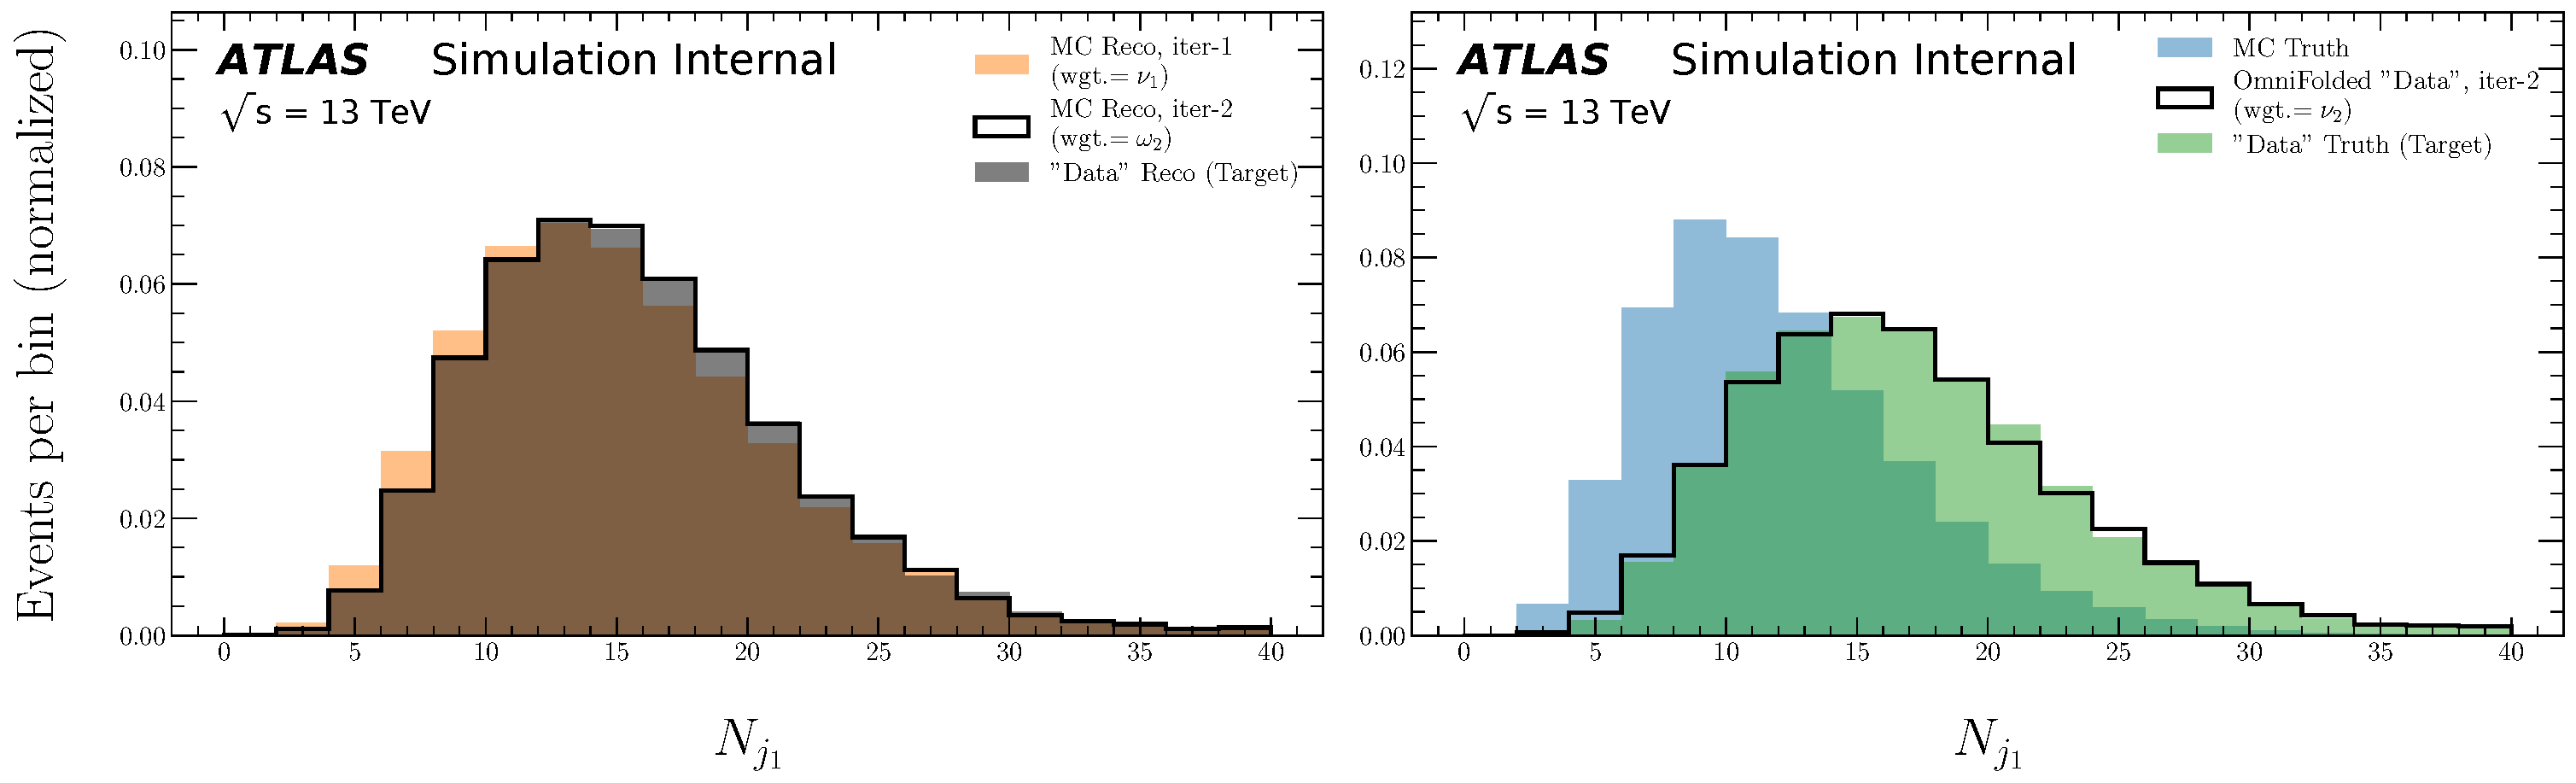
\includegraphics[width=0.85\textwidth]{figures/ATLASOmniFold-StressTest/ATLASOmniFold-StressTestA/UniFold/Ntracks_trackj1/ATLASOmniFold-StressTestA-UniFold-Ntracks_trackj1-Iteration02}}
\phantomcaption
\end{figure}

\begin{figure}[h!]
\centering
\ContinuedFloat
\subfloat[After 3 iterations]{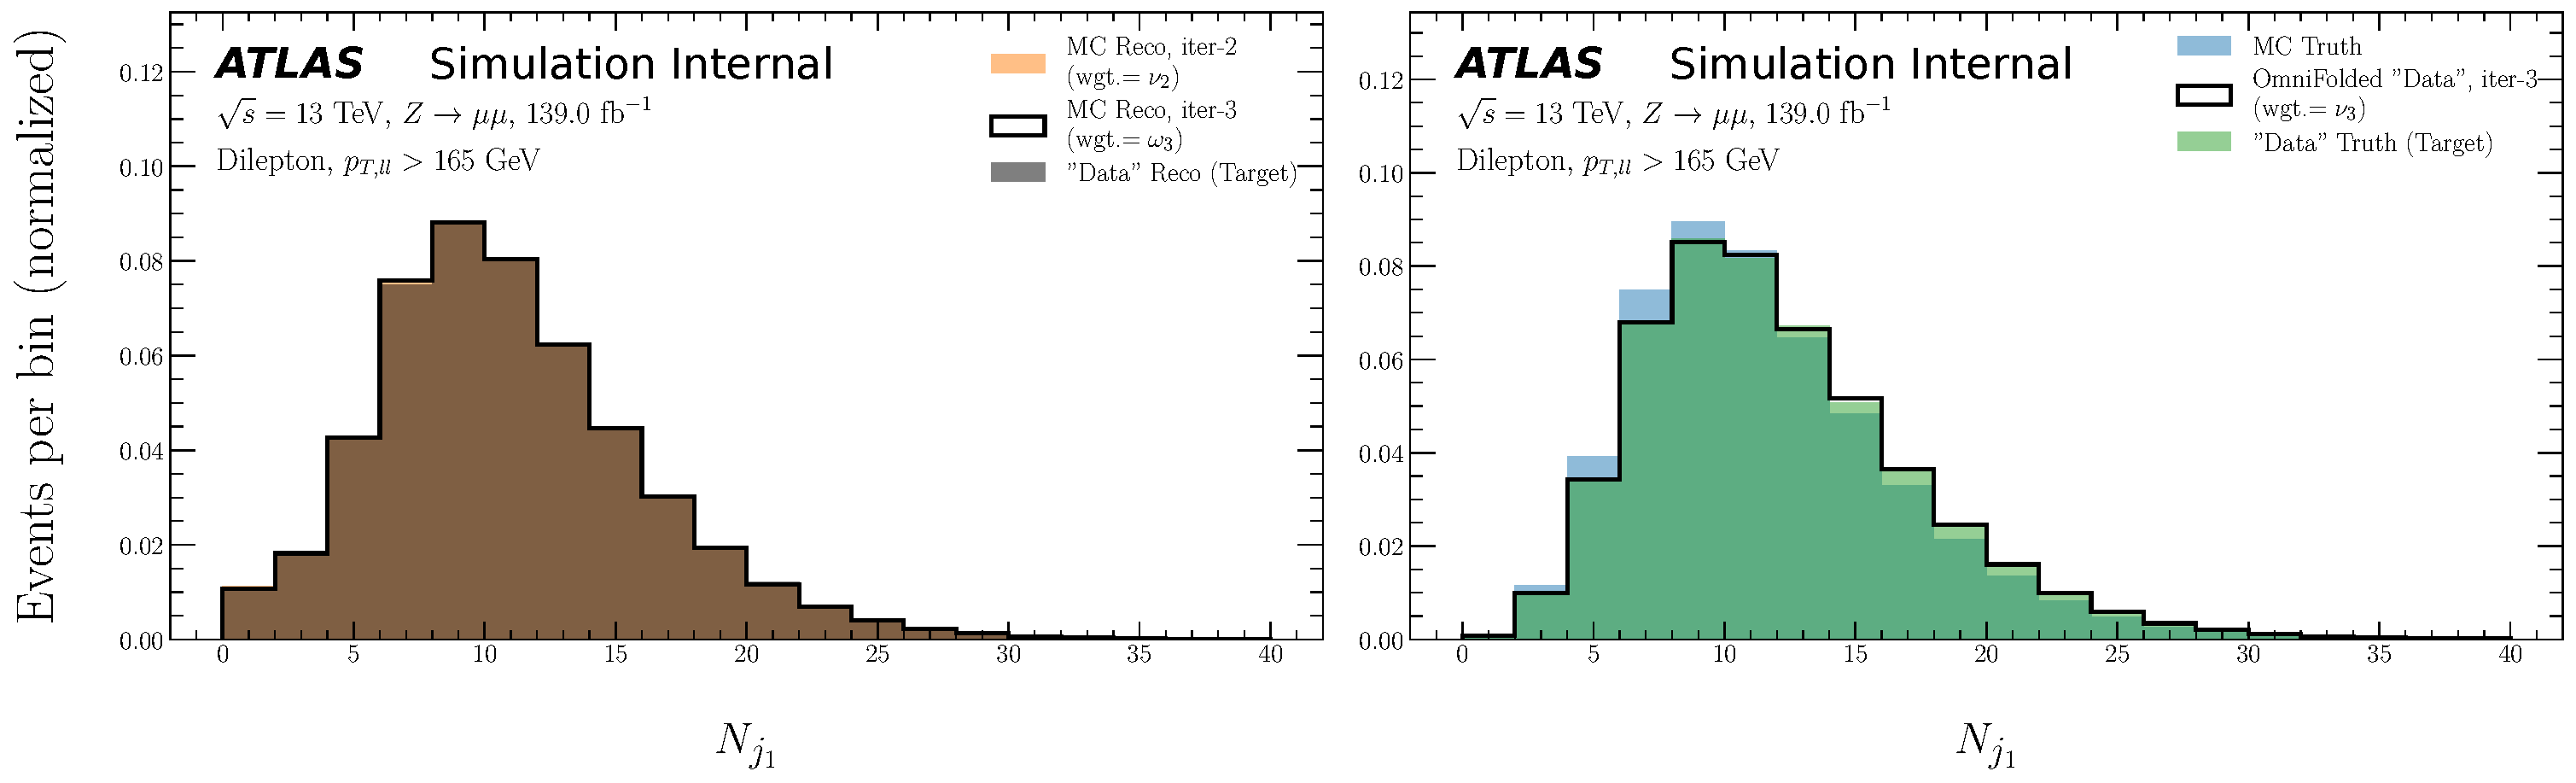
\includegraphics[width=0.85\textwidth]{figures/ATLASOmniFold-StressTest/ATLASOmniFold-StressTestA/UniFold/Ntracks_trackj1/ATLASOmniFold-StressTestA-UniFold-Ntracks_trackj1-Iteration03}}\\
\subfloat[After 4 iterations]{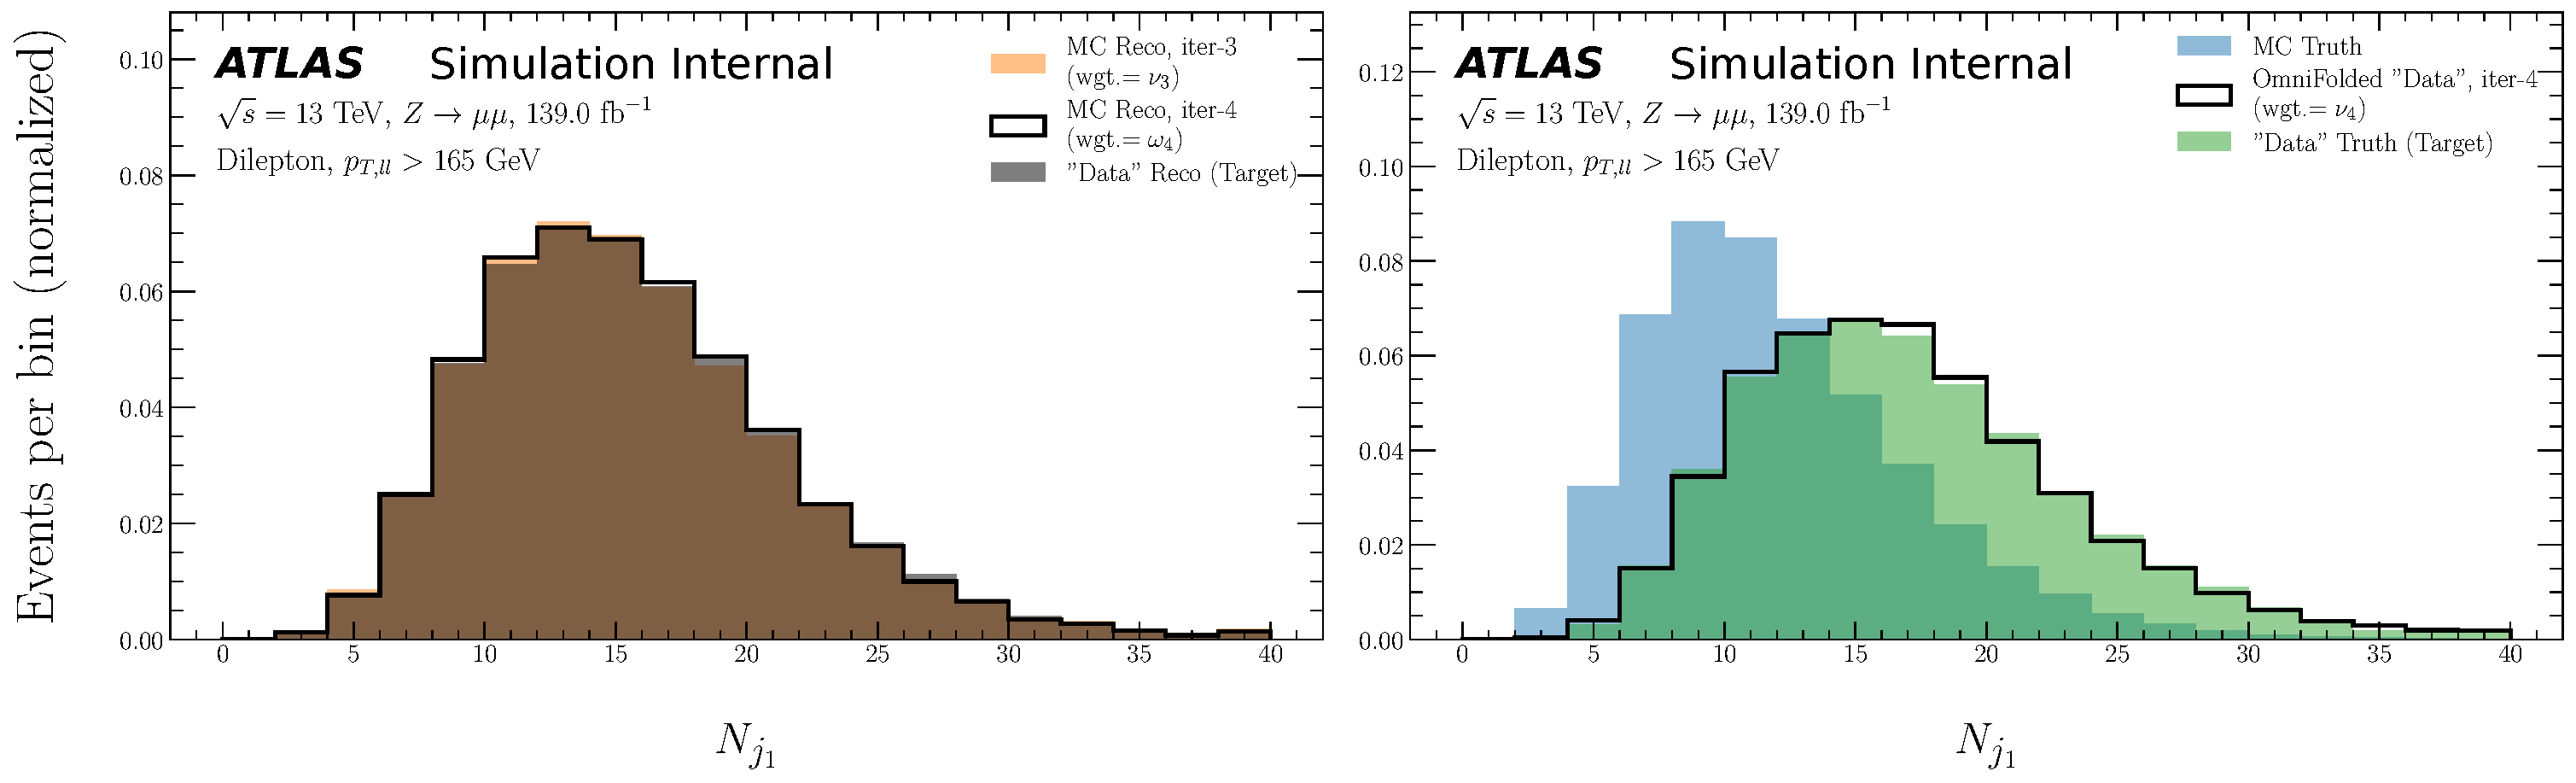
\includegraphics[width=0.85\textwidth]{figures/ATLASOmniFold-StressTest/ATLASOmniFold-StressTestA/UniFold/Ntracks_trackj1/ATLASOmniFold-StressTestA-UniFold-Ntracks_trackj1-Iteration04}}\\
\subfloat[After 5 iterations]{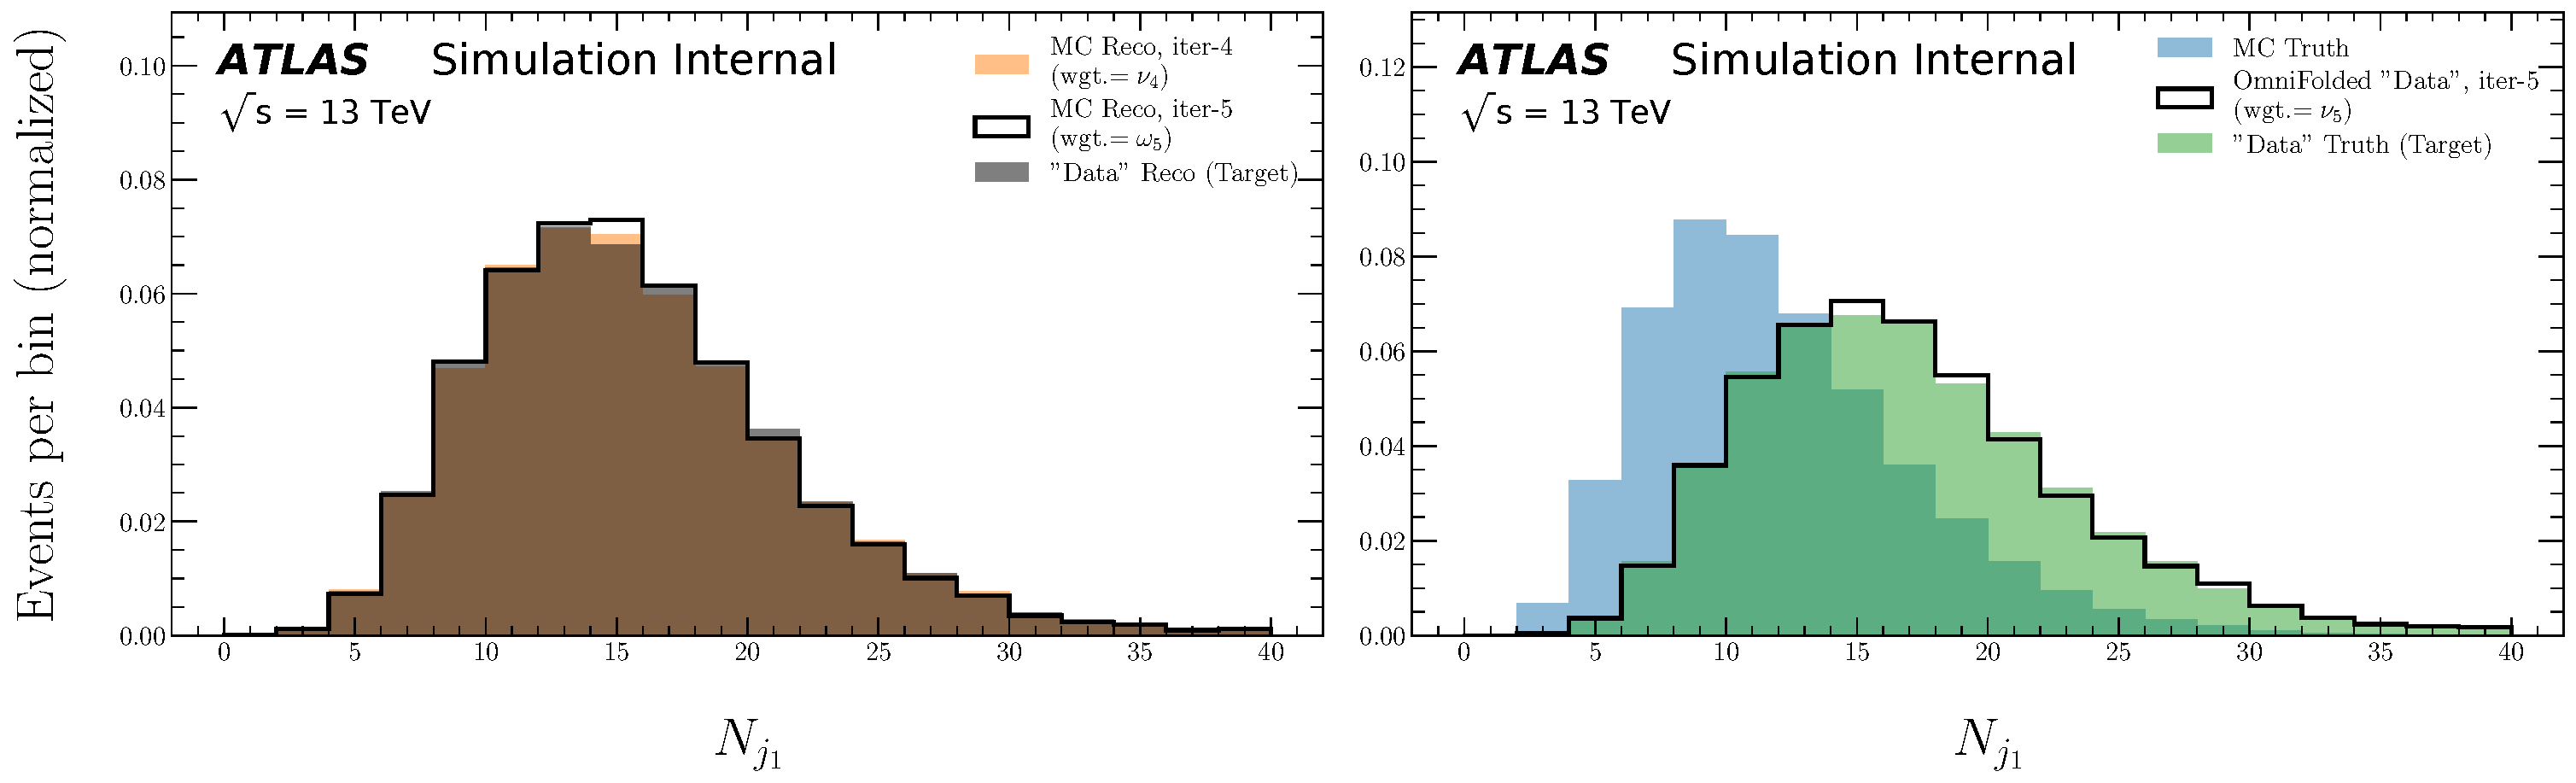
\includegraphics[width=0.85\textwidth]{figures/ATLASOmniFold-StressTest/ATLASOmniFold-StressTestA/UniFold/Ntracks_trackj1/ATLASOmniFold-StressTestA-UniFold-Ntracks_trackj1-Iteration05}}\\
\subfloat[After 6 iterations]{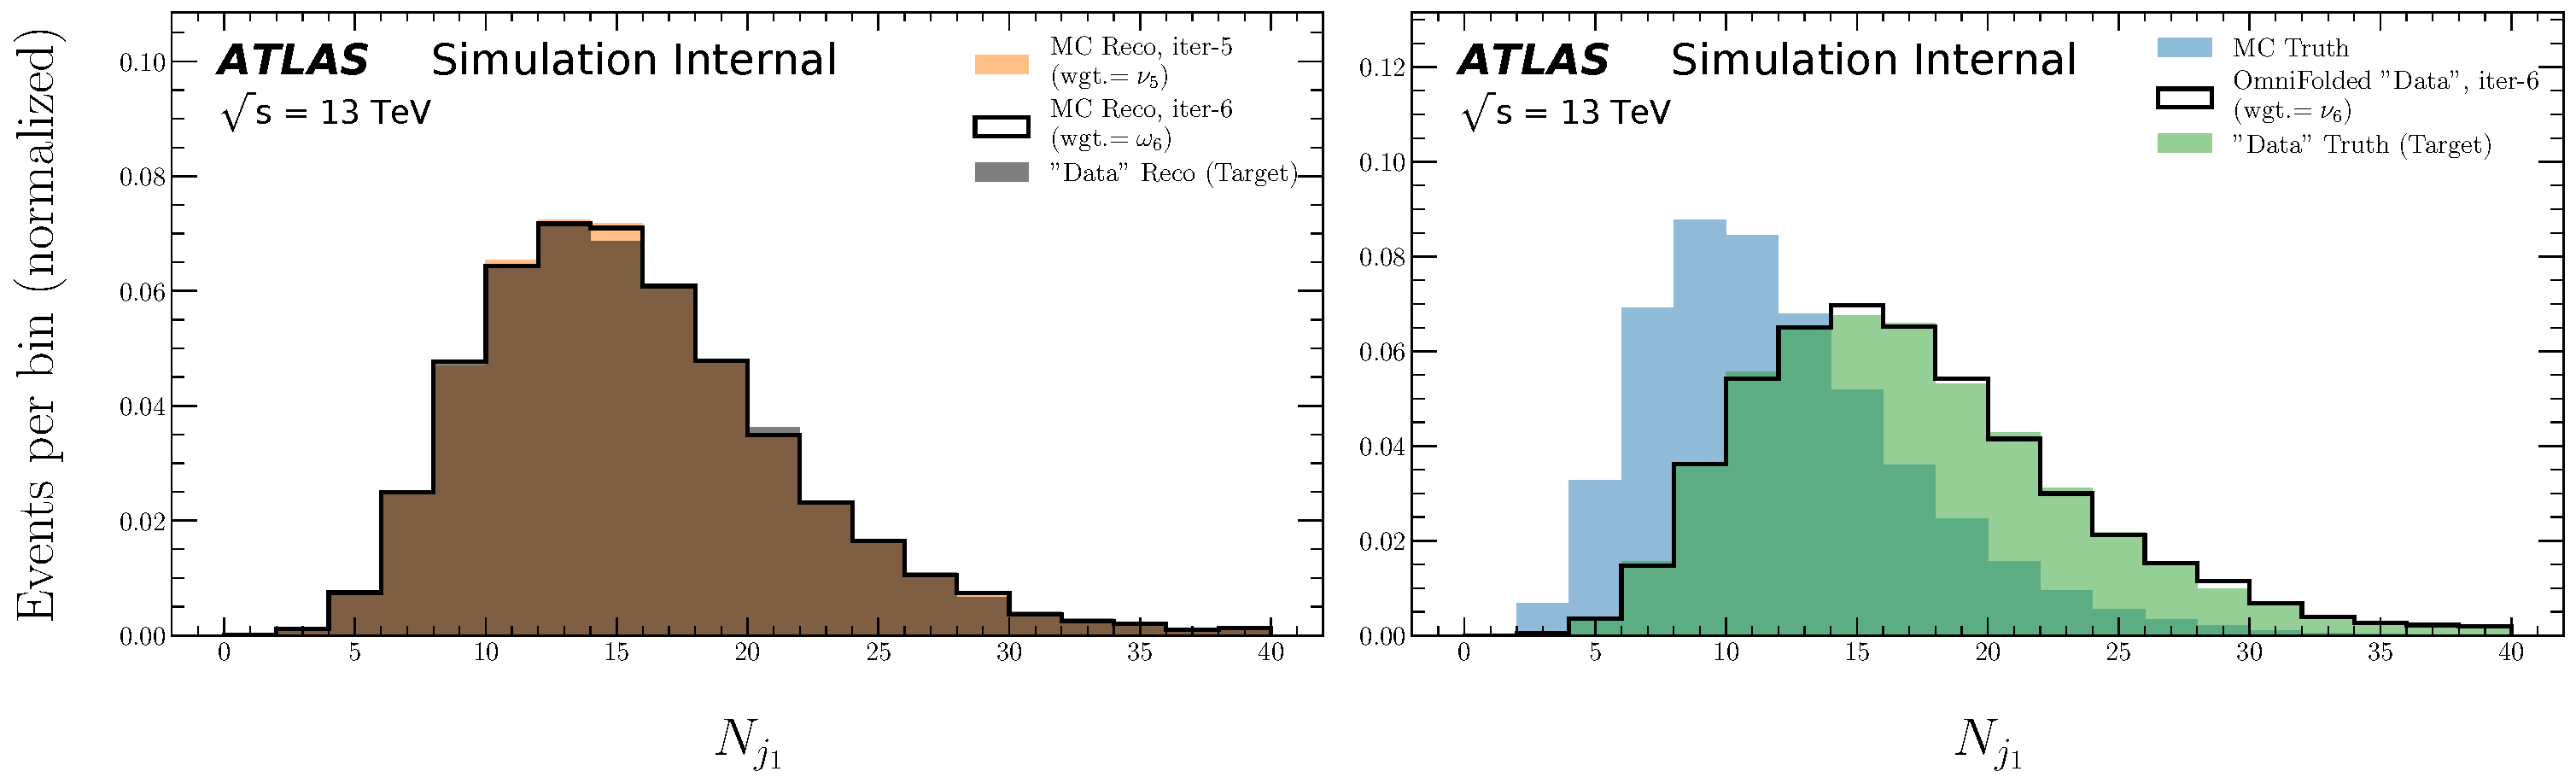
\includegraphics[width=0.85\textwidth]{figures/ATLASOmniFold-StressTest/ATLASOmniFold-StressTestA/UniFold/Ntracks_trackj1/ATLASOmniFold-StressTestA-UniFold-Ntracks_trackj1-Iteration06}}
\caption{A stress test for UniFold applied to the leading track jet constituent multiplicity.}
\label{fig:stressa_Ntracks_trackj1}
\end{figure}

\clearpage

\paragraph{MultiFold} Stress weights for the 16-dimensional MultiFold are shown in Fig.~\ref{fig:stressa_weightsMulti}.  These are constructed by adding the stress weights for each observable as defined by Eq.~\ref{eq:stressweights} (the MC weight only enters once).  Figures~\ref{fig:stressa_massMultih} and~\ref{fig:stressa_Ntracks_trackj1Multi} are examples for the leading track jet mass and the number of tracks inside jets.  Additional examples can be found in App~\ref{sec:stressmultifolddet}.

\begin{figure}[h!]
\centering
\subfloat[Weights]{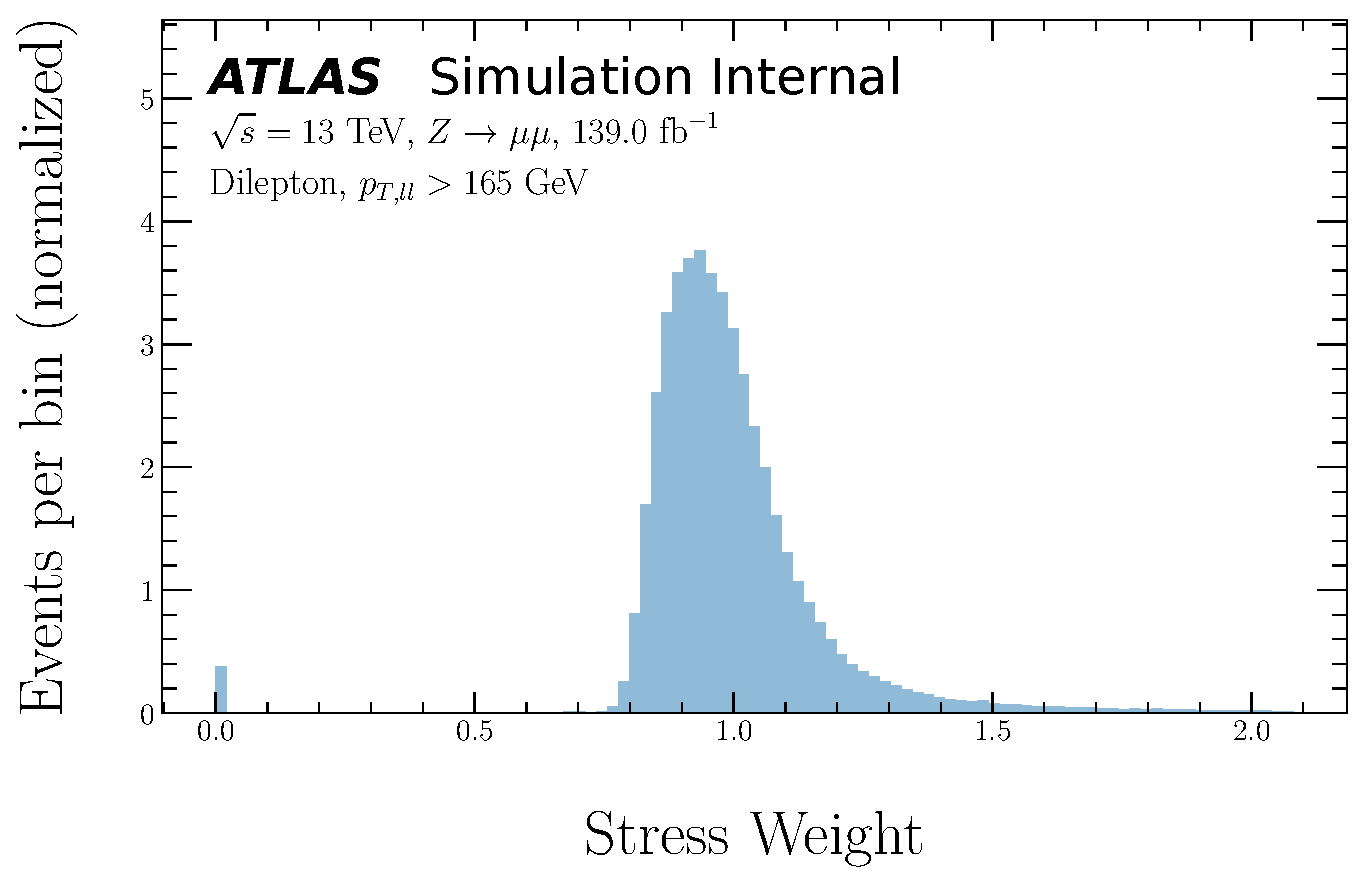
\includegraphics[width=0.45\textwidth]{figures/ATLASOmniFold-StressTest/ATLASOmniFold-StressTestA/MultiFold/ATLASOmniFold-StressTestA-MultiFold--StressWeightsHist.pdf}}
\caption{A stress weights for the deterministic weight option for MultiFold.  Unlike UniFold, there is now only one set of weights for all 16 observables instead of a different set of weights for each observable.}
\label{fig:stressa_weightsMulti}
\end{figure}

\begin{figure}[h!]
\centering
\subfloat[Input histograms]{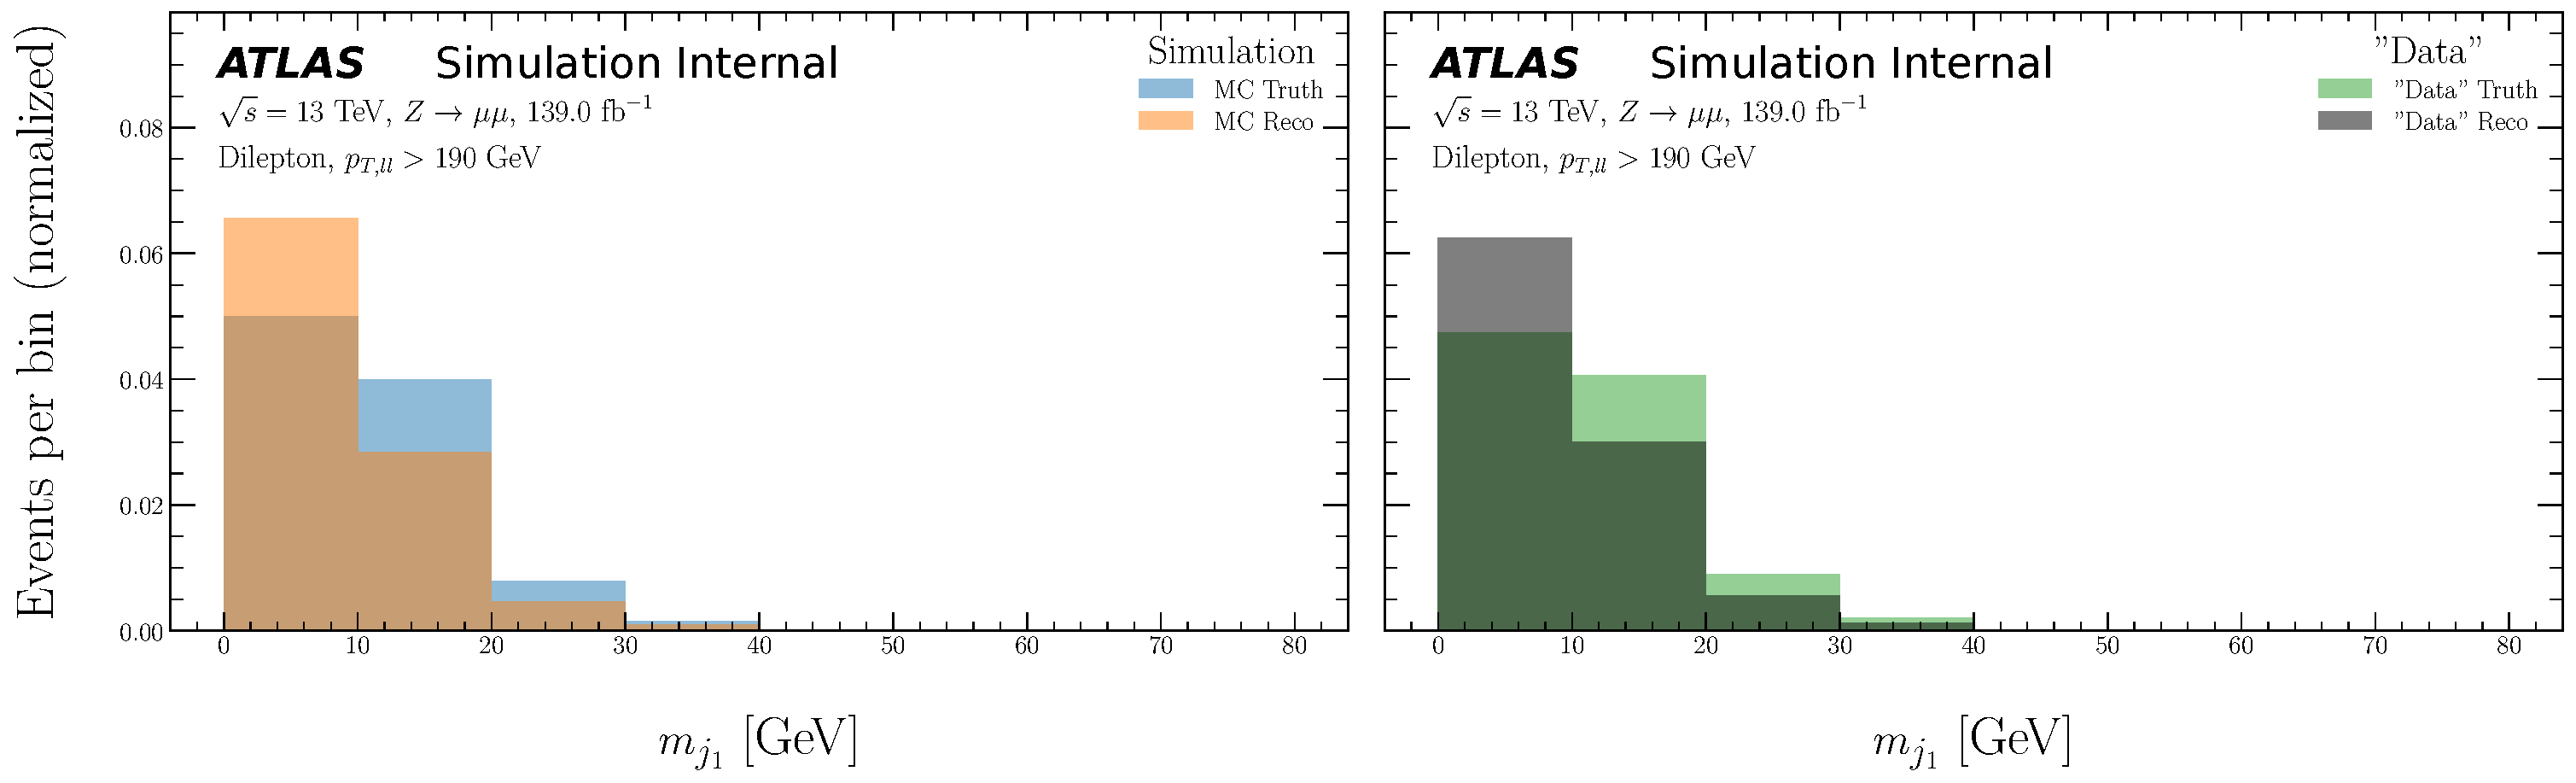
\includegraphics[width=0.85\textwidth]{figures/ATLASOmniFold-StressTest/ATLASOmniFold-StressTestA/MultiFold/m_trackj1/ATLASOmniFold-StressTestA-MultiFold-m_trackj1-Distributions}}\\
\subfloat[After 1 iteration]{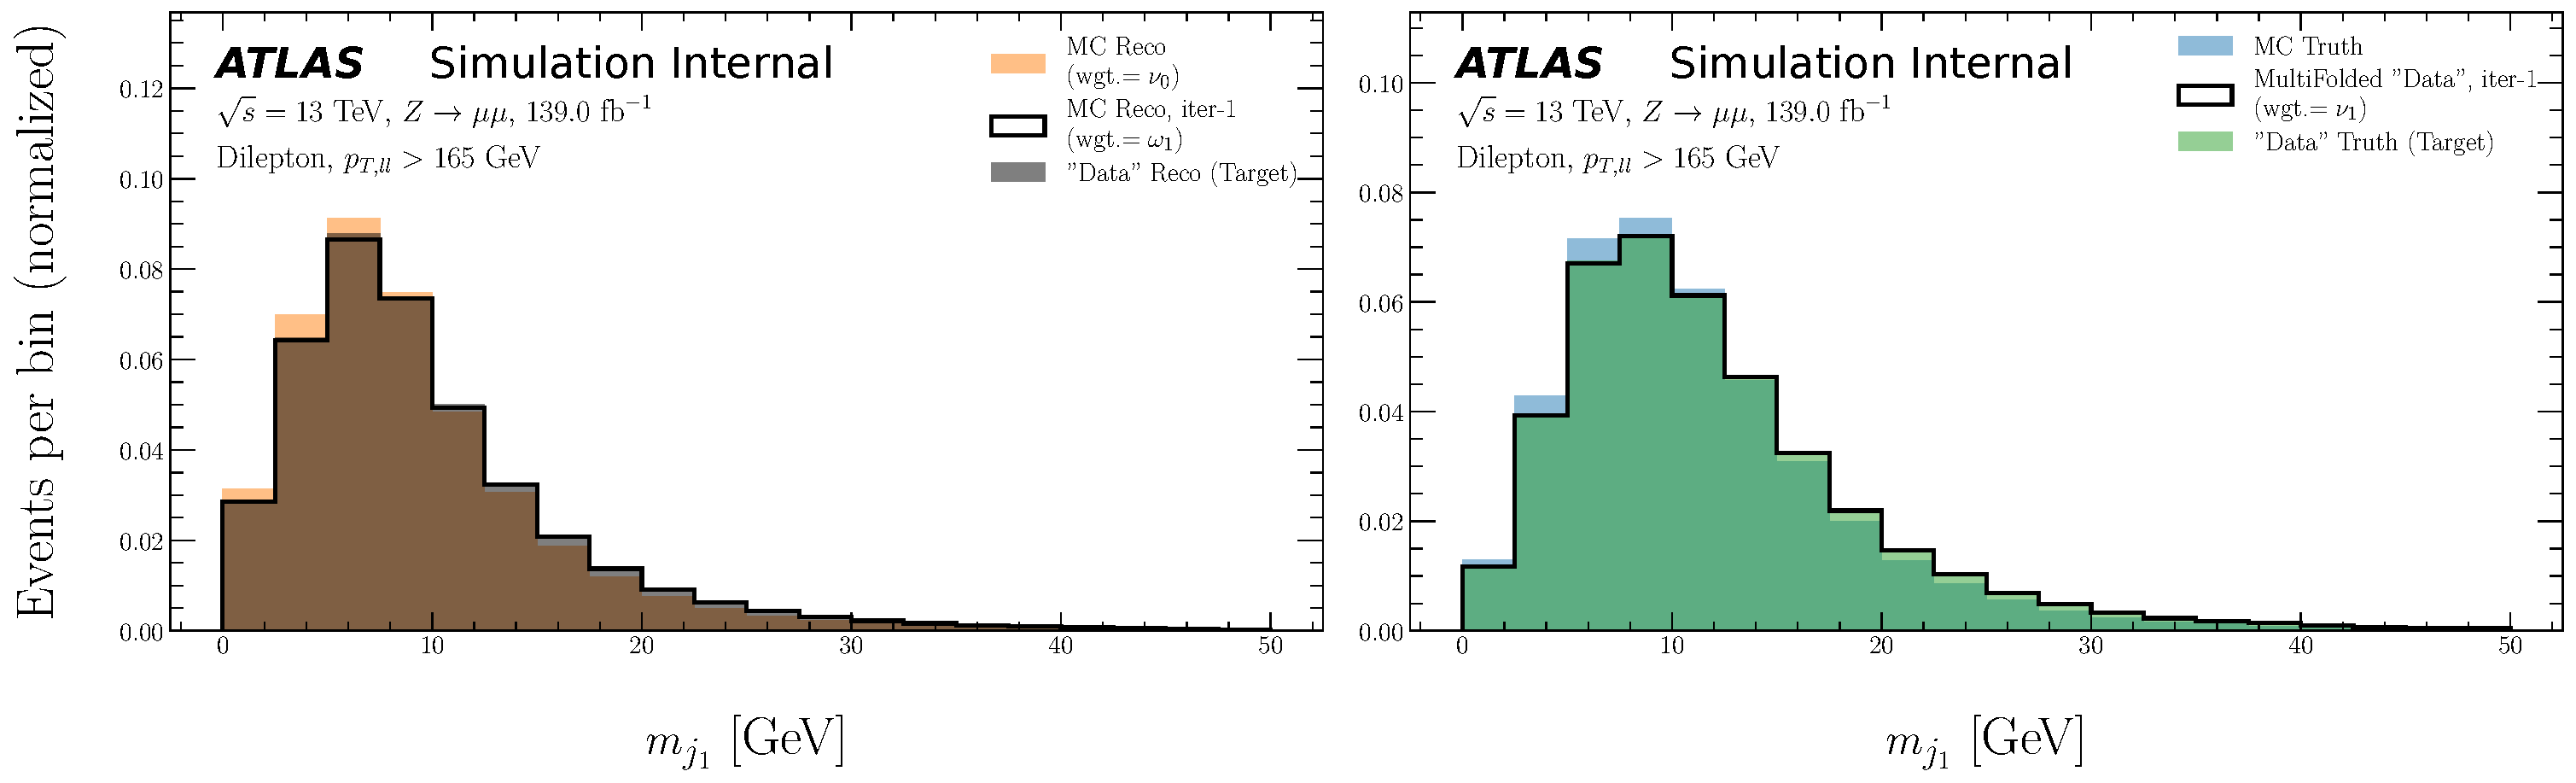
\includegraphics[width=0.85\textwidth]{figures/ATLASOmniFold-StressTest/ATLASOmniFold-StressTestA/MultiFold/m_trackj1/ATLASOmniFold-StressTestA-MultiFold-m_trackj1-Iteration01}}\\
\subfloat[After 2 iterations]{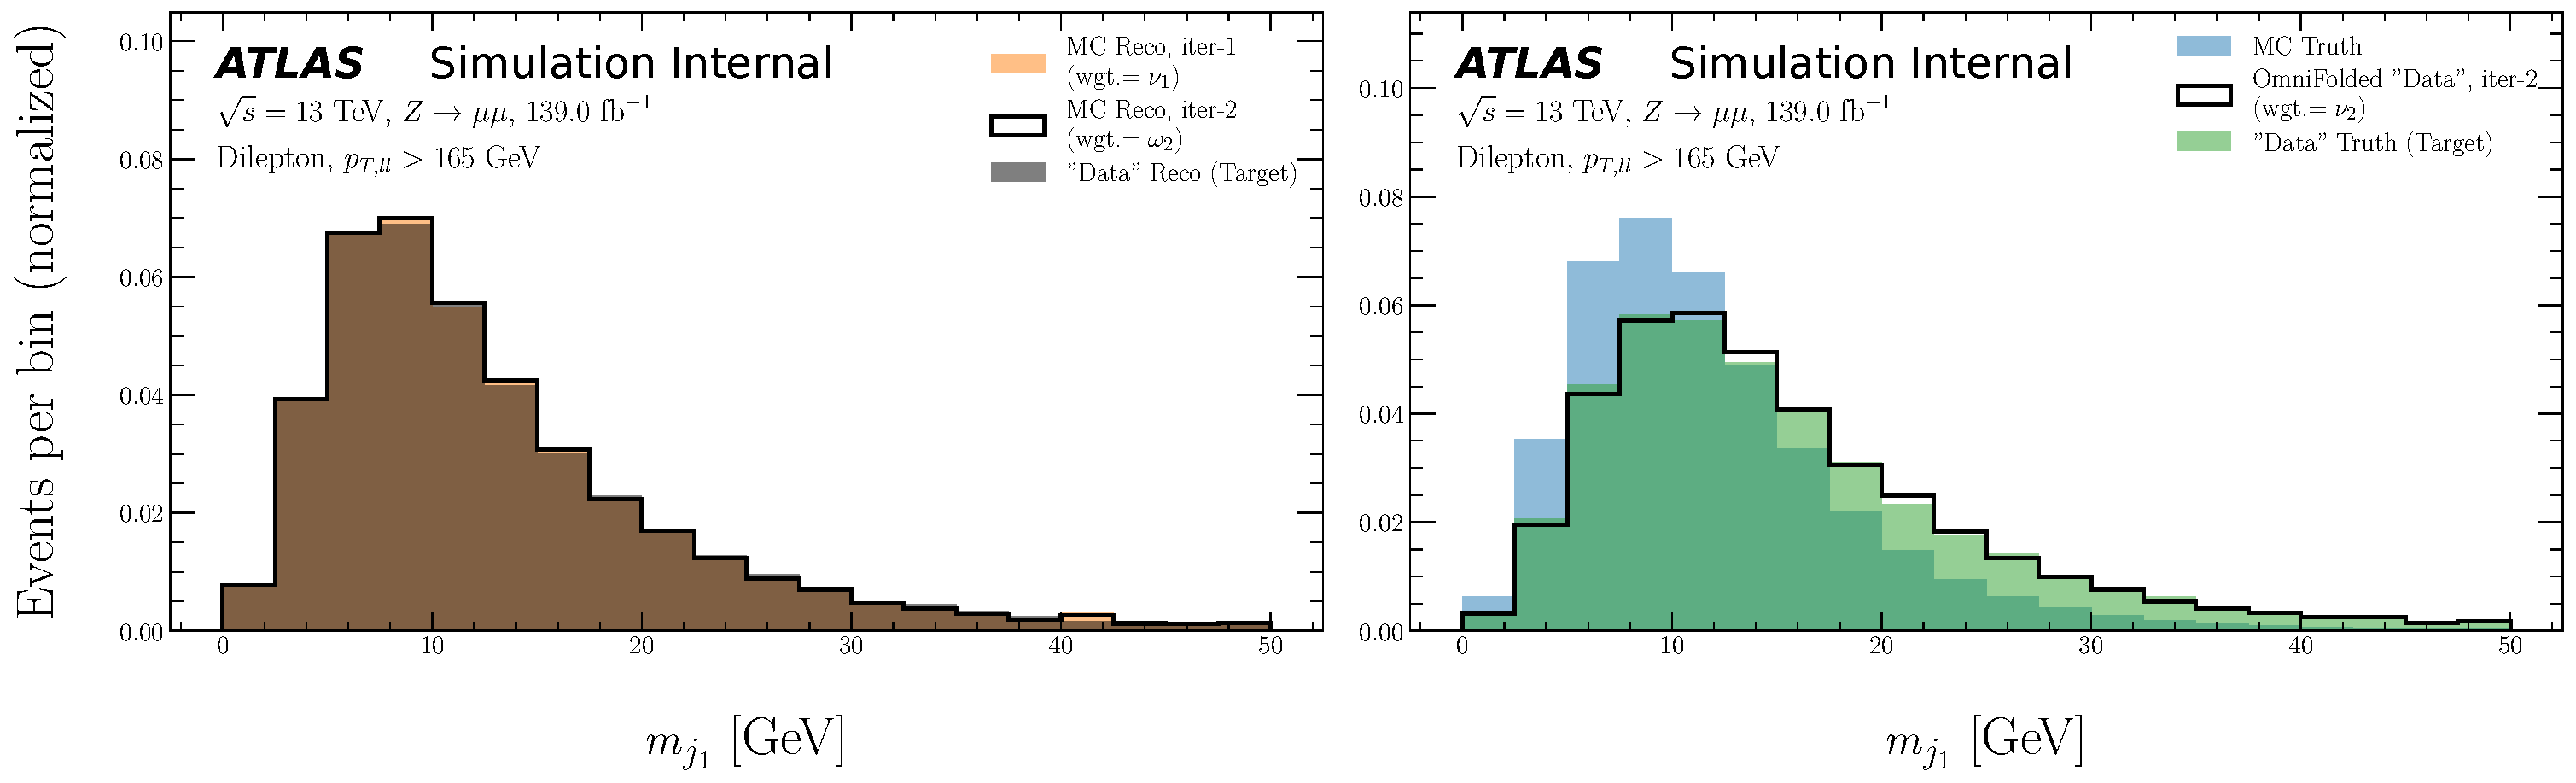
\includegraphics[width=0.85\textwidth]{figures/ATLASOmniFold-StressTest/ATLASOmniFold-StressTestA/MultiFold/m_trackj1/ATLASOmniFold-StressTestA-MultiFold-m_trackj1-Iteration02}}
\phantomcaption
\end{figure}

\begin{figure}[h!]
\centering
\ContinuedFloat
\subfloat[After 3 iterations]{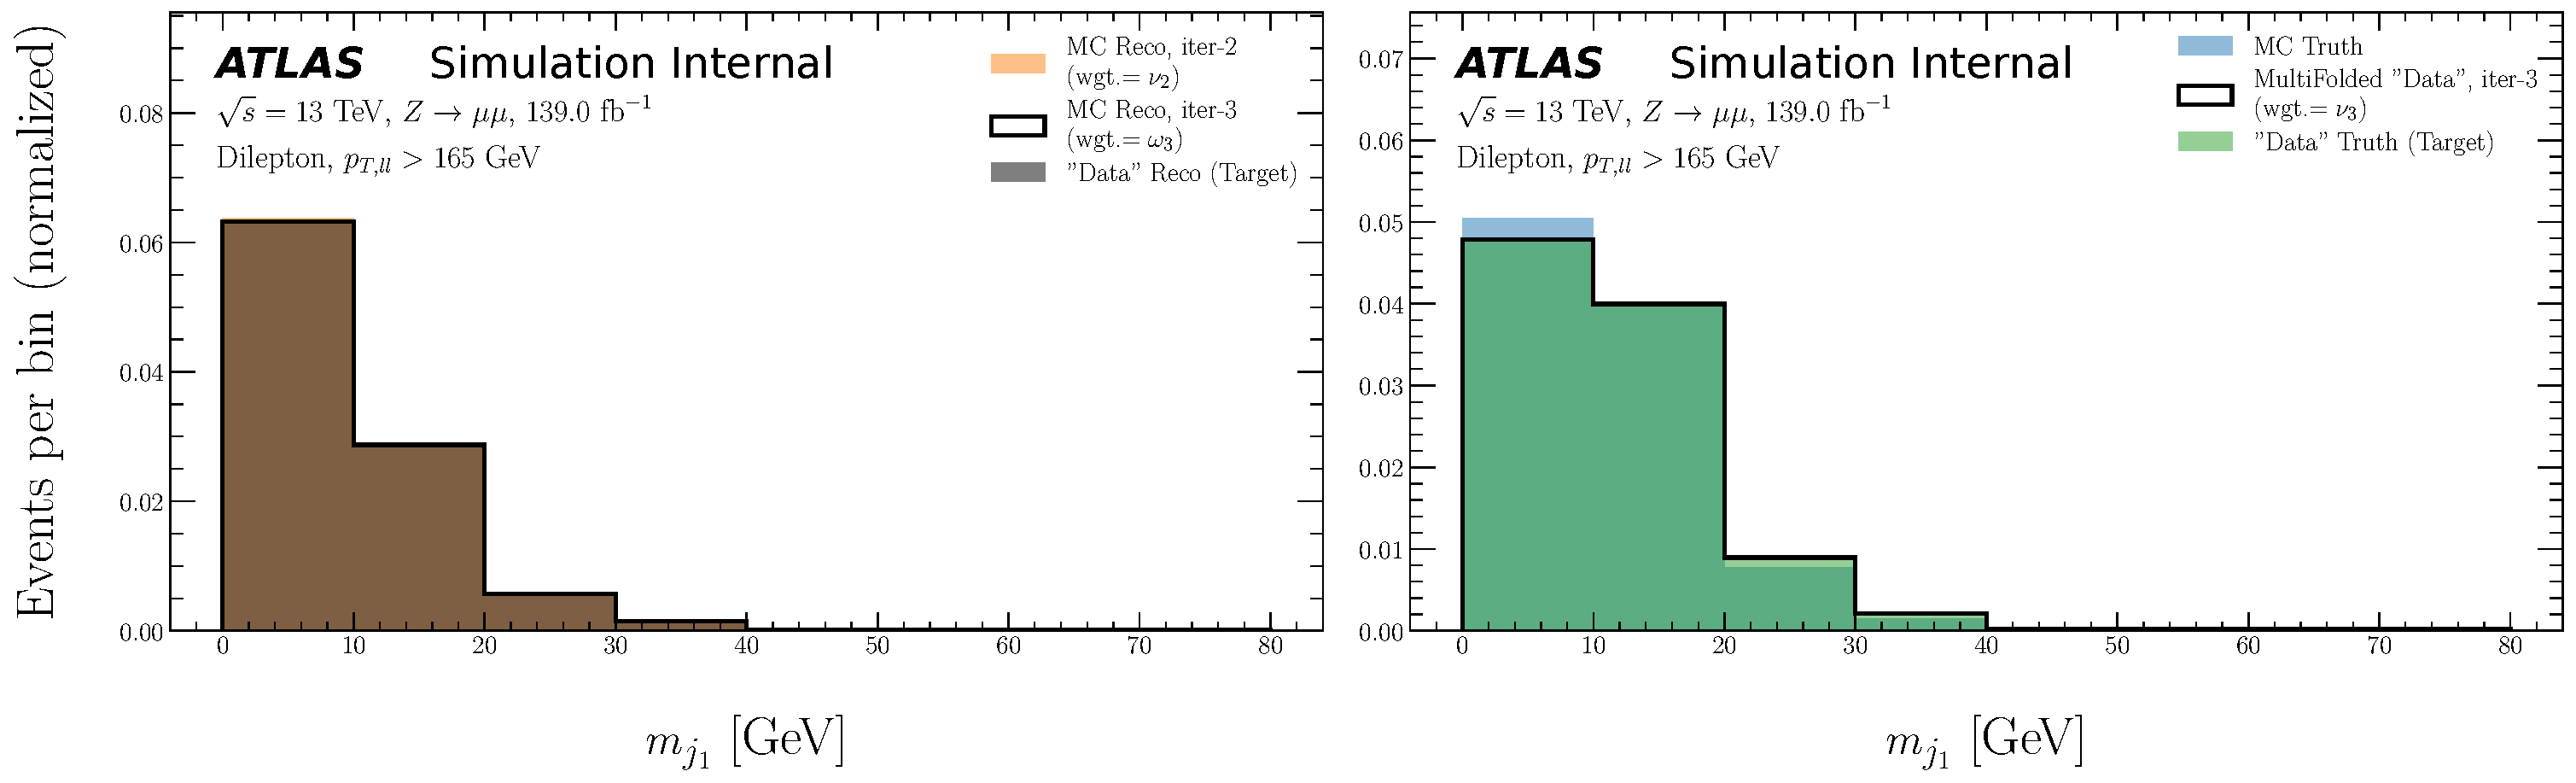
\includegraphics[width=0.85\textwidth]{figures/ATLASOmniFold-StressTest/ATLASOmniFold-StressTestA/MultiFold/m_trackj1/ATLASOmniFold-StressTestA-MultiFold-m_trackj1-Iteration03}}\\
\subfloat[After 4 iterations]{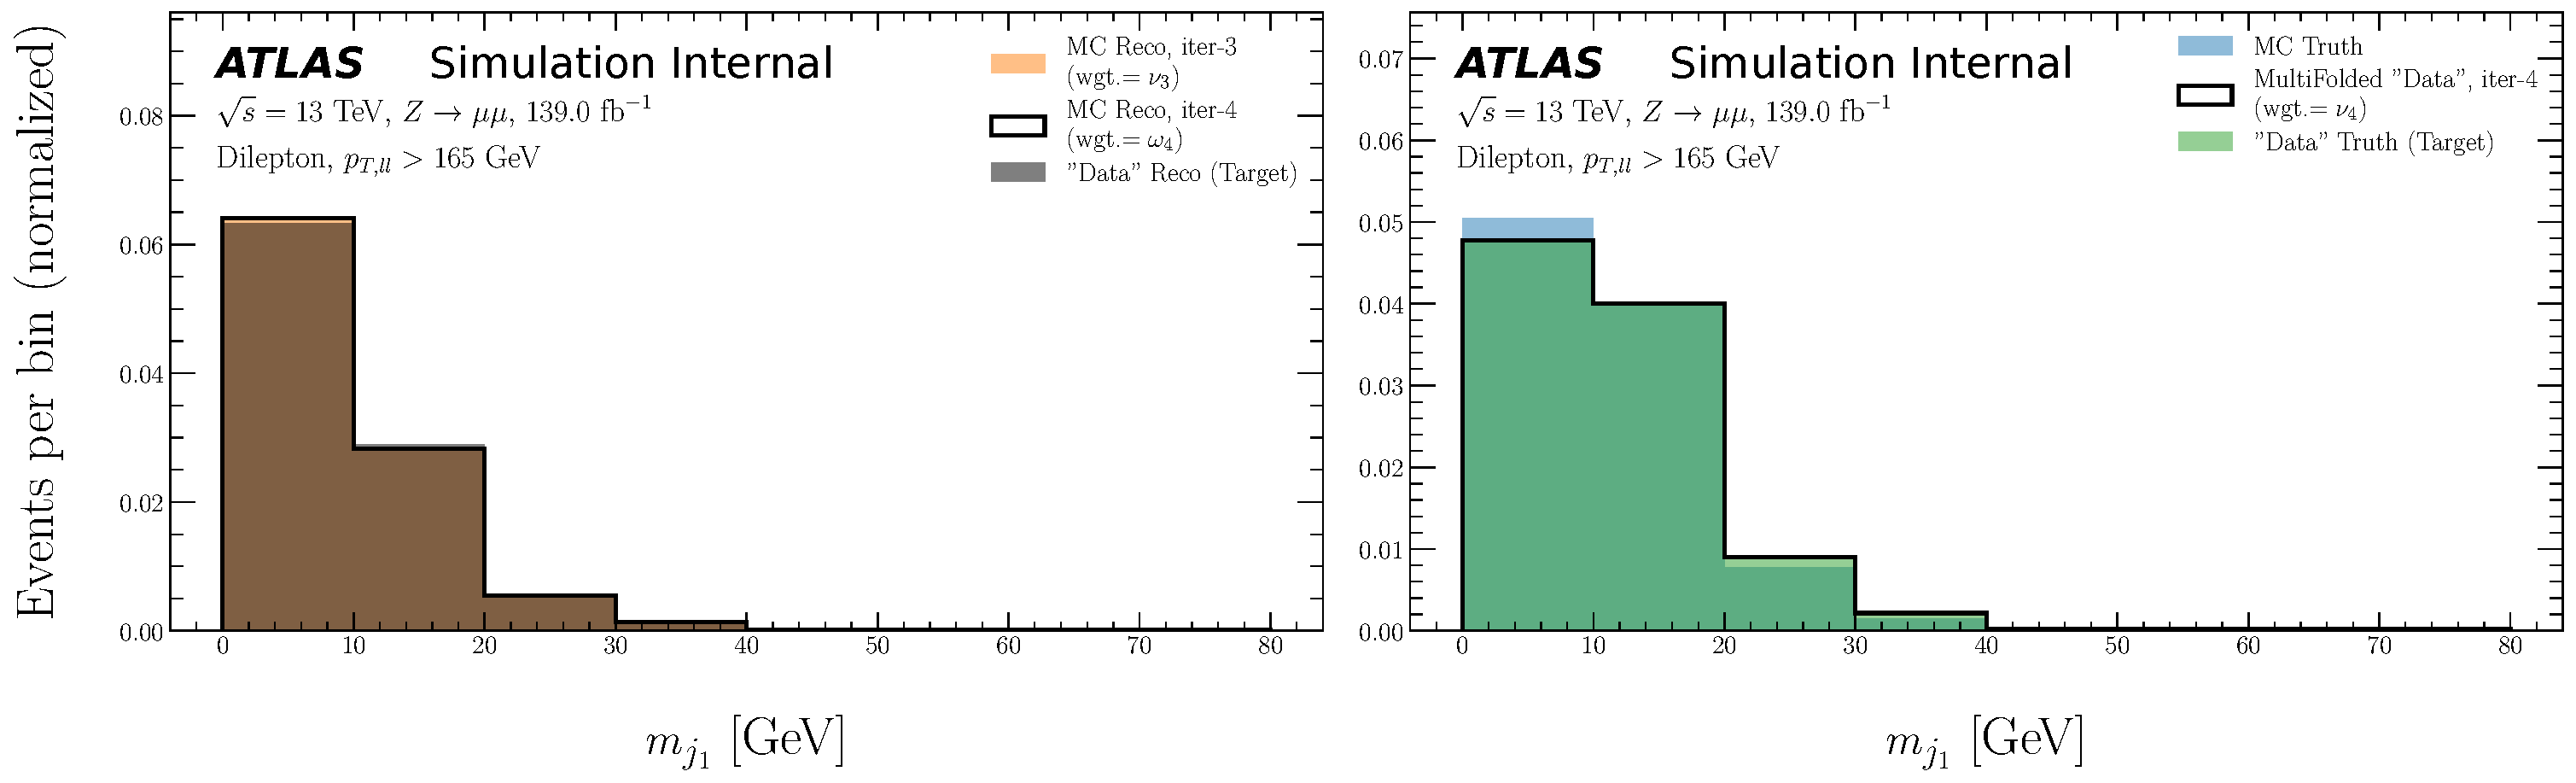
\includegraphics[width=0.85\textwidth]{figures/ATLASOmniFold-StressTest/ATLASOmniFold-StressTestA/MultiFold/m_trackj1/ATLASOmniFold-StressTestA-MultiFold-m_trackj1-Iteration04}}\\
\subfloat[After 5 iterations]{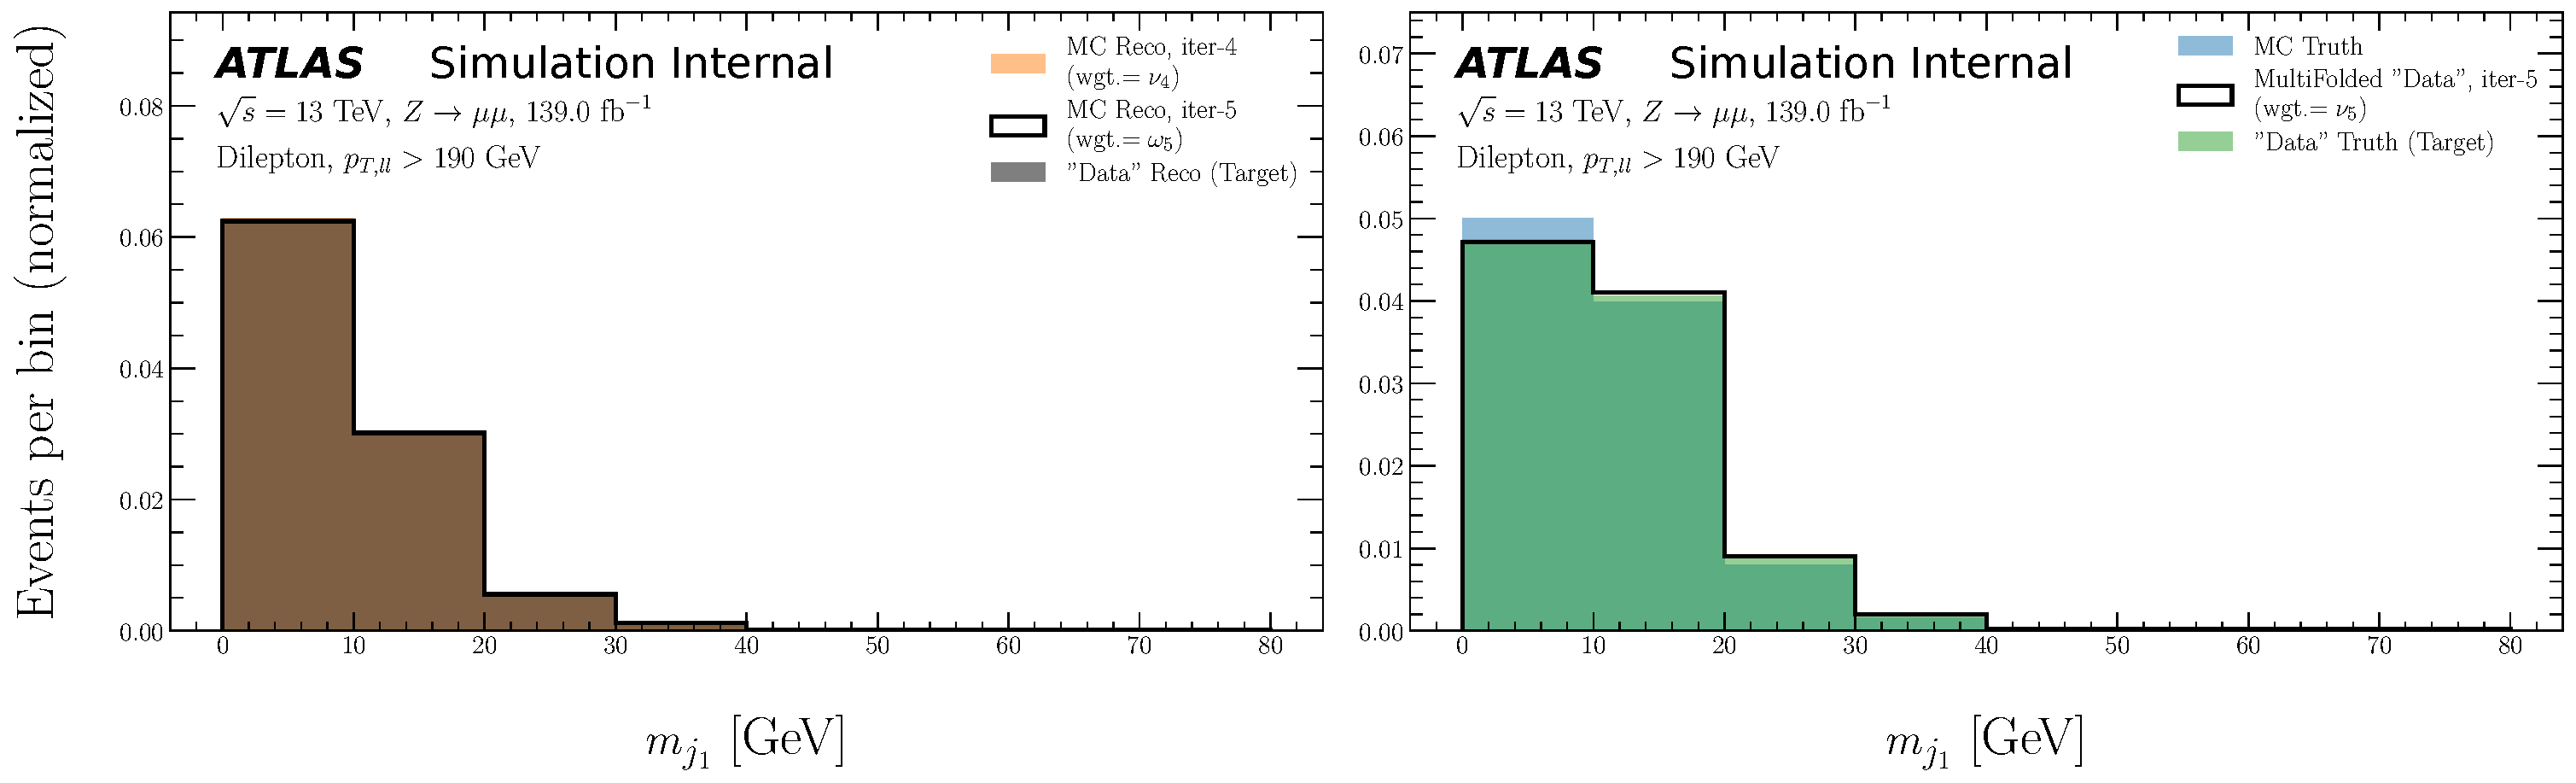
\includegraphics[width=0.85\textwidth]{figures/ATLASOmniFold-StressTest/ATLASOmniFold-StressTestA/MultiFold/m_trackj1/ATLASOmniFold-StressTestA-MultiFold-m_trackj1-Iteration05}}\\
\subfloat[After 6 iterations]{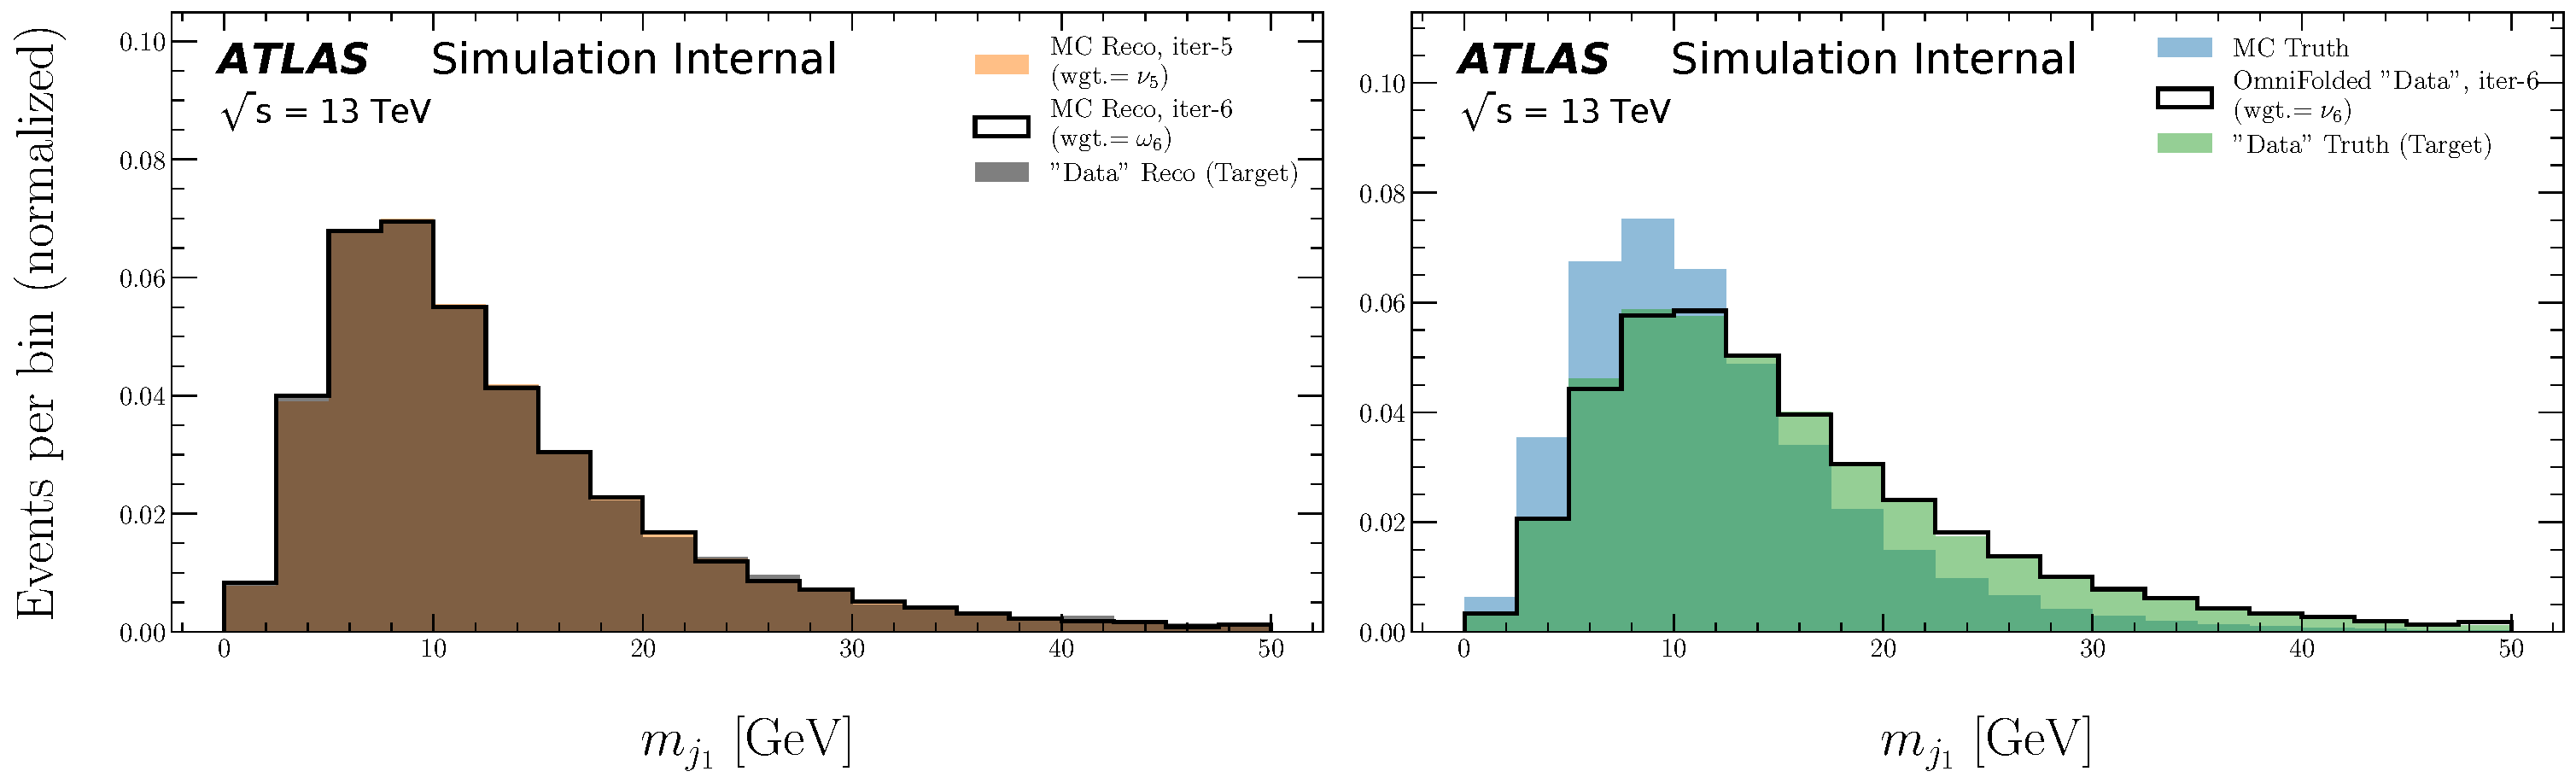
\includegraphics[width=0.85\textwidth]{figures/ATLASOmniFold-StressTest/ATLASOmniFold-StressTestA/MultiFold/m_trackj1/ATLASOmniFold-StressTestA-MultiFold-m_trackj1-Iteration06}}
\caption{A stress test for MultiFold using deterministic weights applied to the leading track jet mass.}
\label{fig:stressa_massMultih}
\end{figure}

\begin{figure}[h!]
\centering
\subfloat[Input histograms]{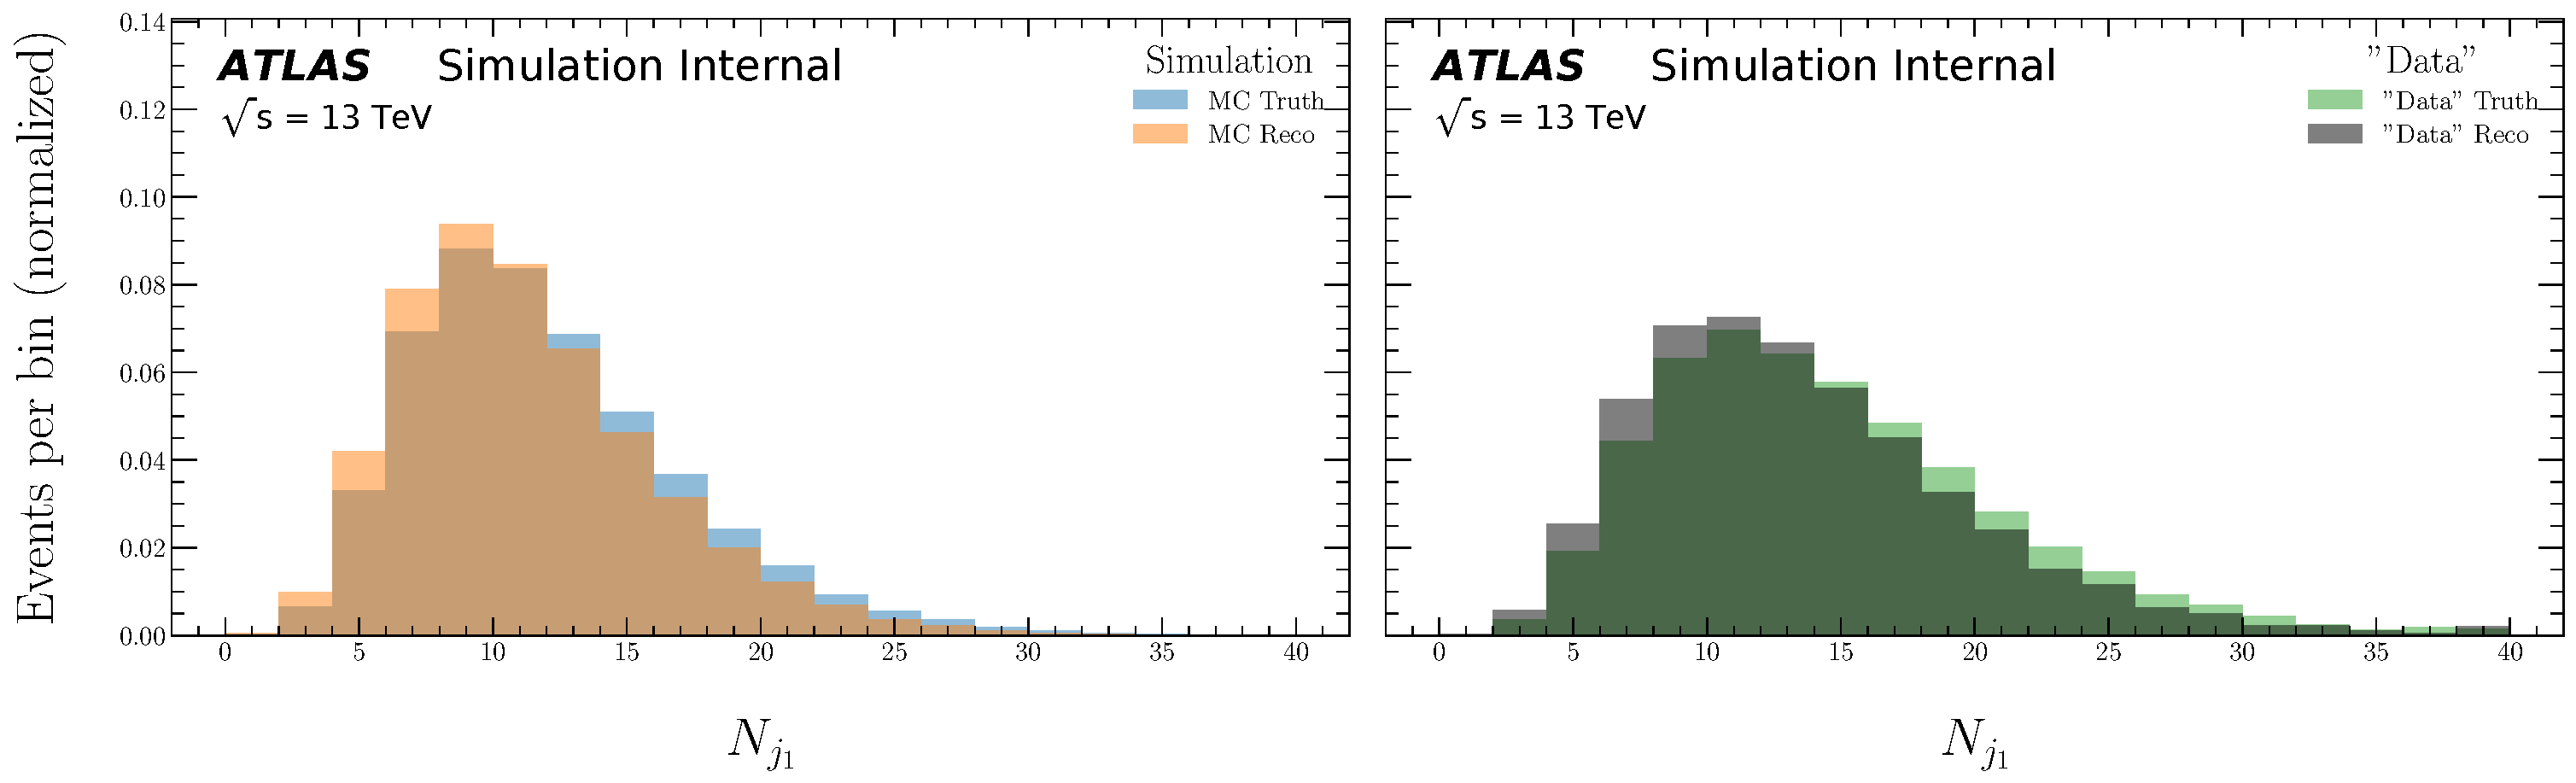
\includegraphics[width=0.85\textwidth]{figures/ATLASOmniFold-StressTest/ATLASOmniFold-StressTestA/MultiFold/Ntracks_trackj1/ATLASOmniFold-StressTestA-MultiFold-Ntracks_trackj1-Distributions}}\\
\subfloat[After 1 iteration]{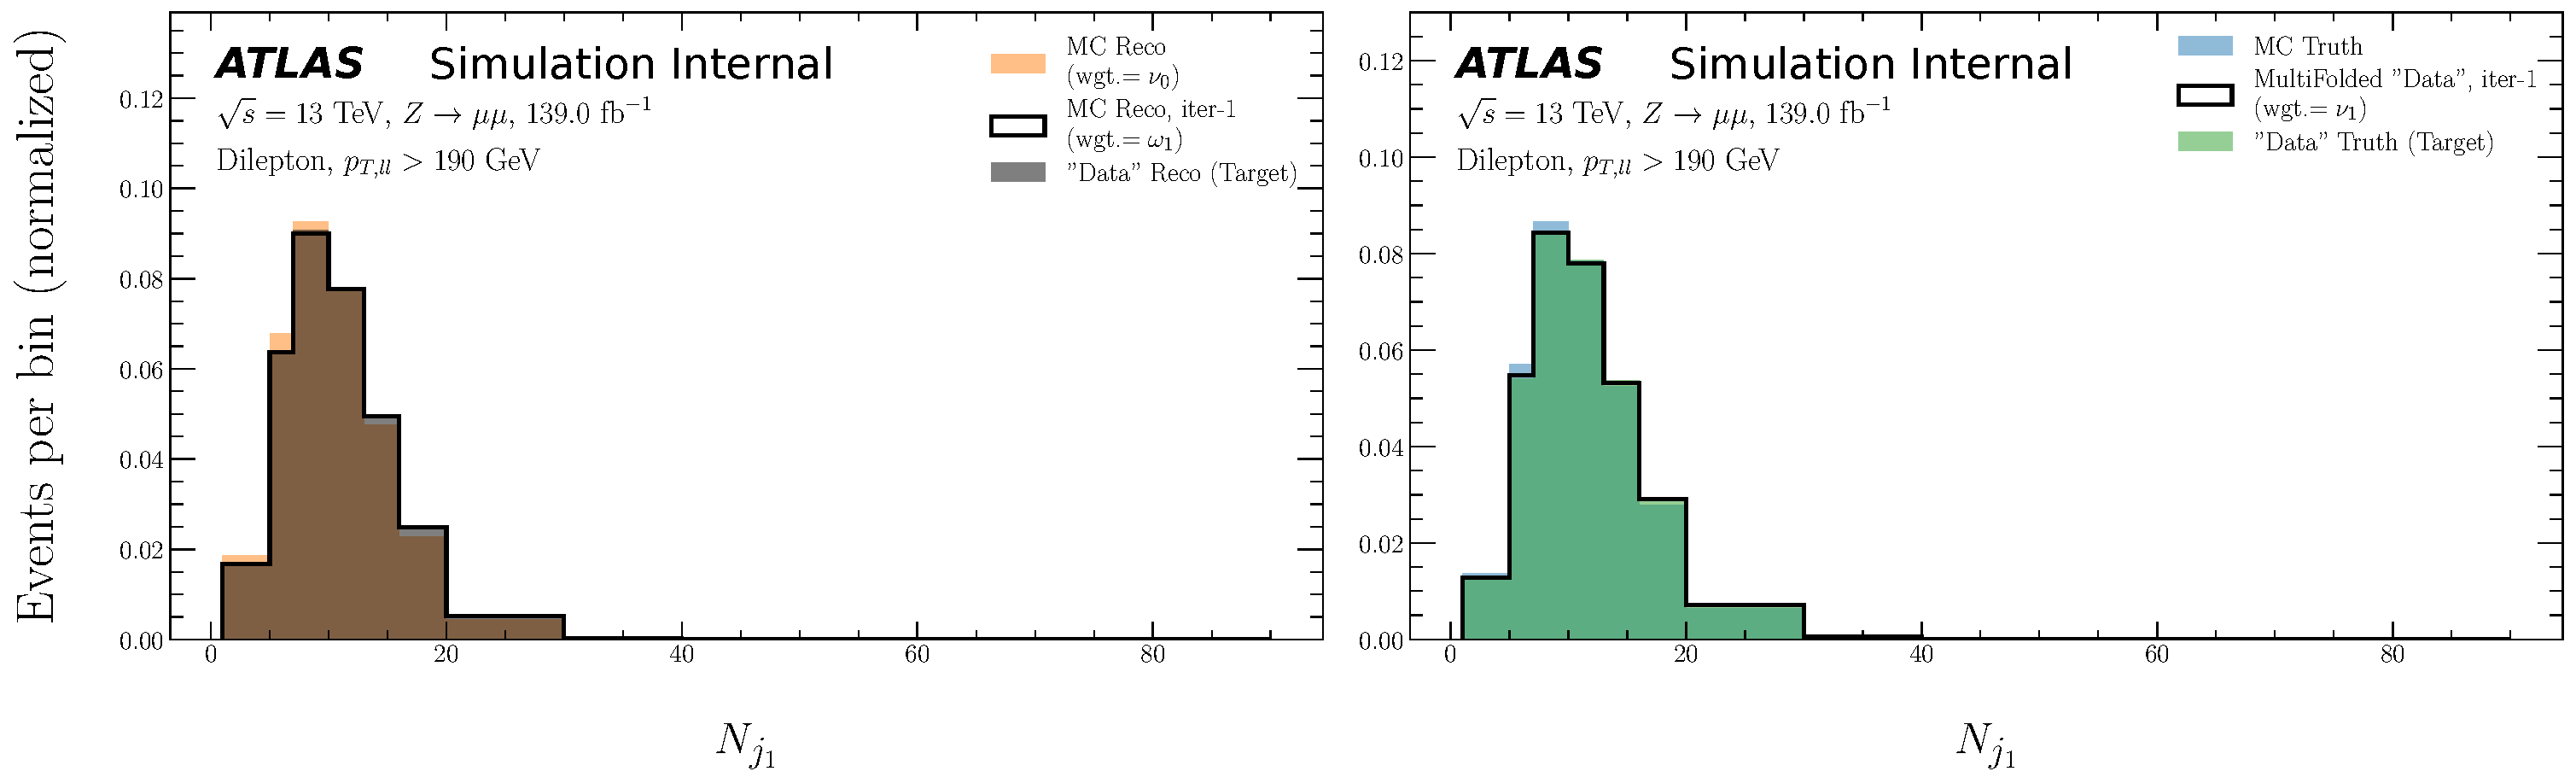
\includegraphics[width=0.85\textwidth]{figures/ATLASOmniFold-StressTest/ATLASOmniFold-StressTestA/MultiFold/Ntracks_trackj1/ATLASOmniFold-StressTestA-MultiFold-Ntracks_trackj1-Iteration01}}\\
\subfloat[After 2 iterations]{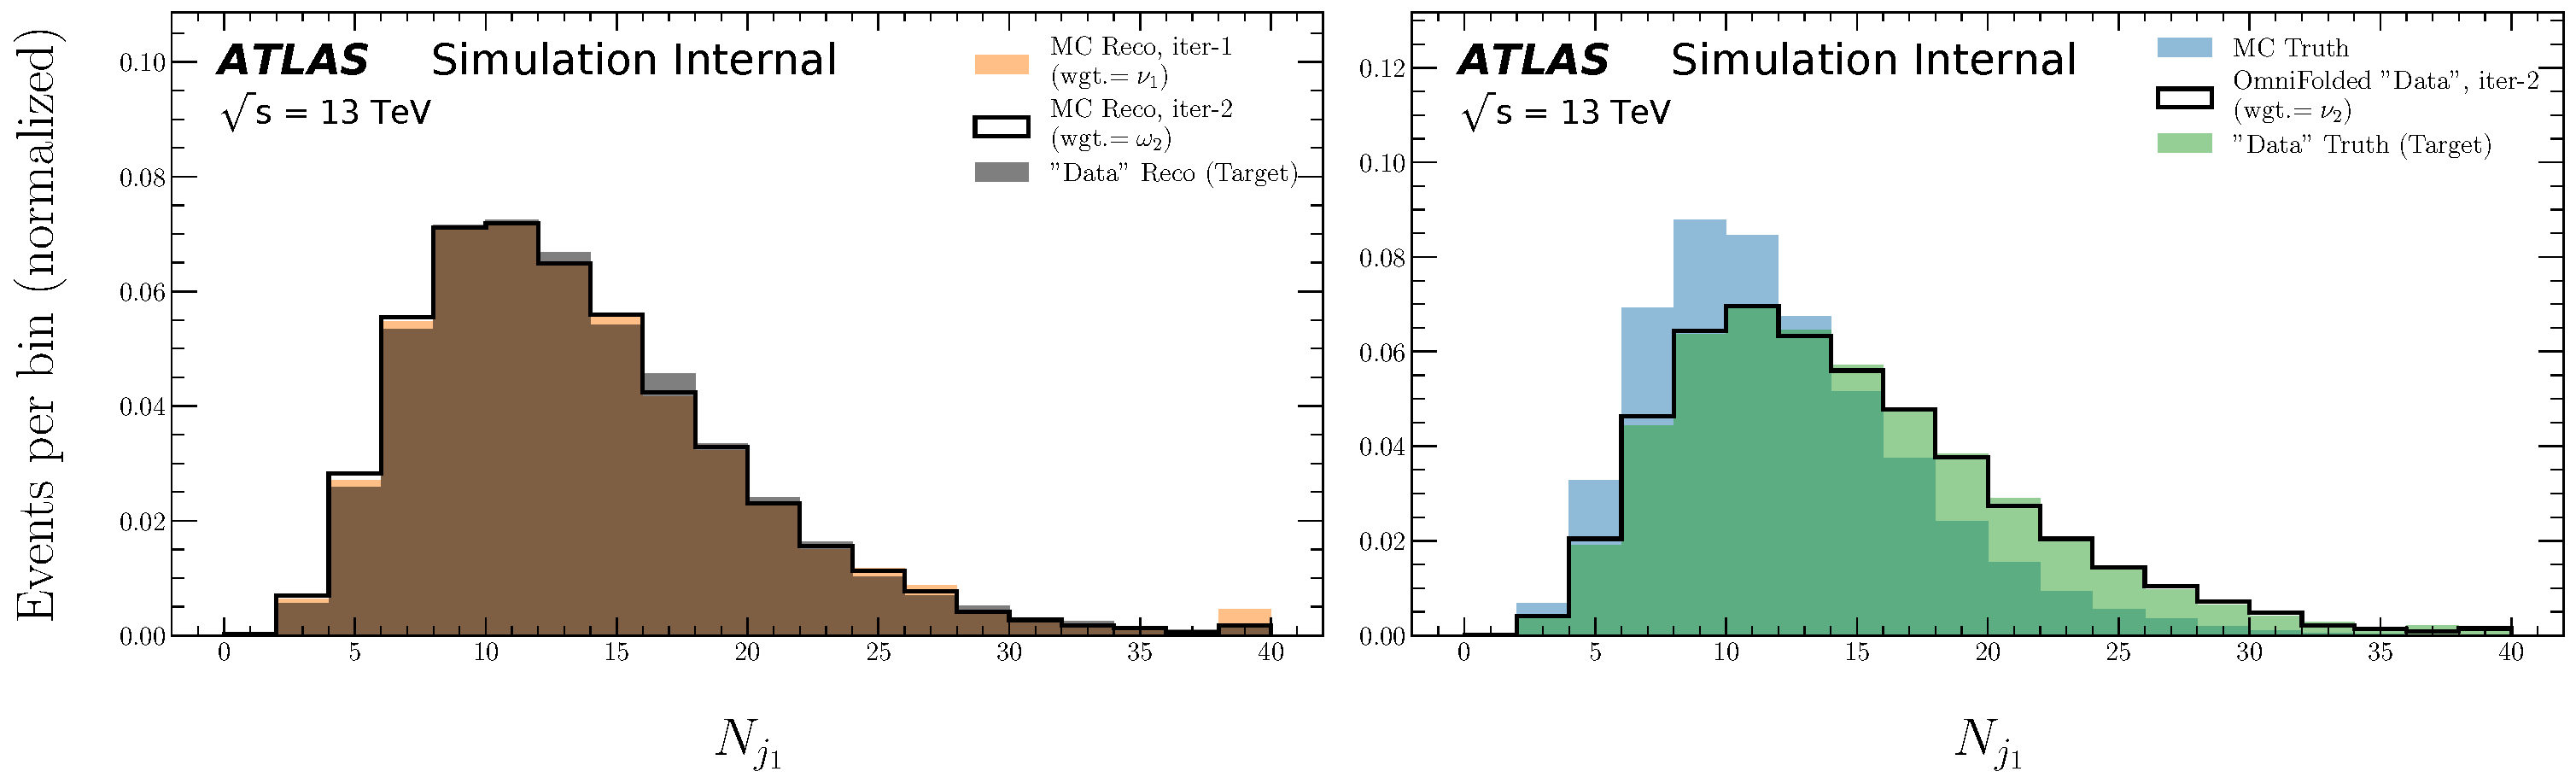
\includegraphics[width=0.85\textwidth]{figures/ATLASOmniFold-StressTest/ATLASOmniFold-StressTestA/MultiFold/Ntracks_trackj1/ATLASOmniFold-StressTestA-MultiFold-Ntracks_trackj1-Iteration02}}
\phantomcaption
\end{figure}

\begin{figure}[h!]
\centering
\ContinuedFloat
\subfloat[After 3 iterations]{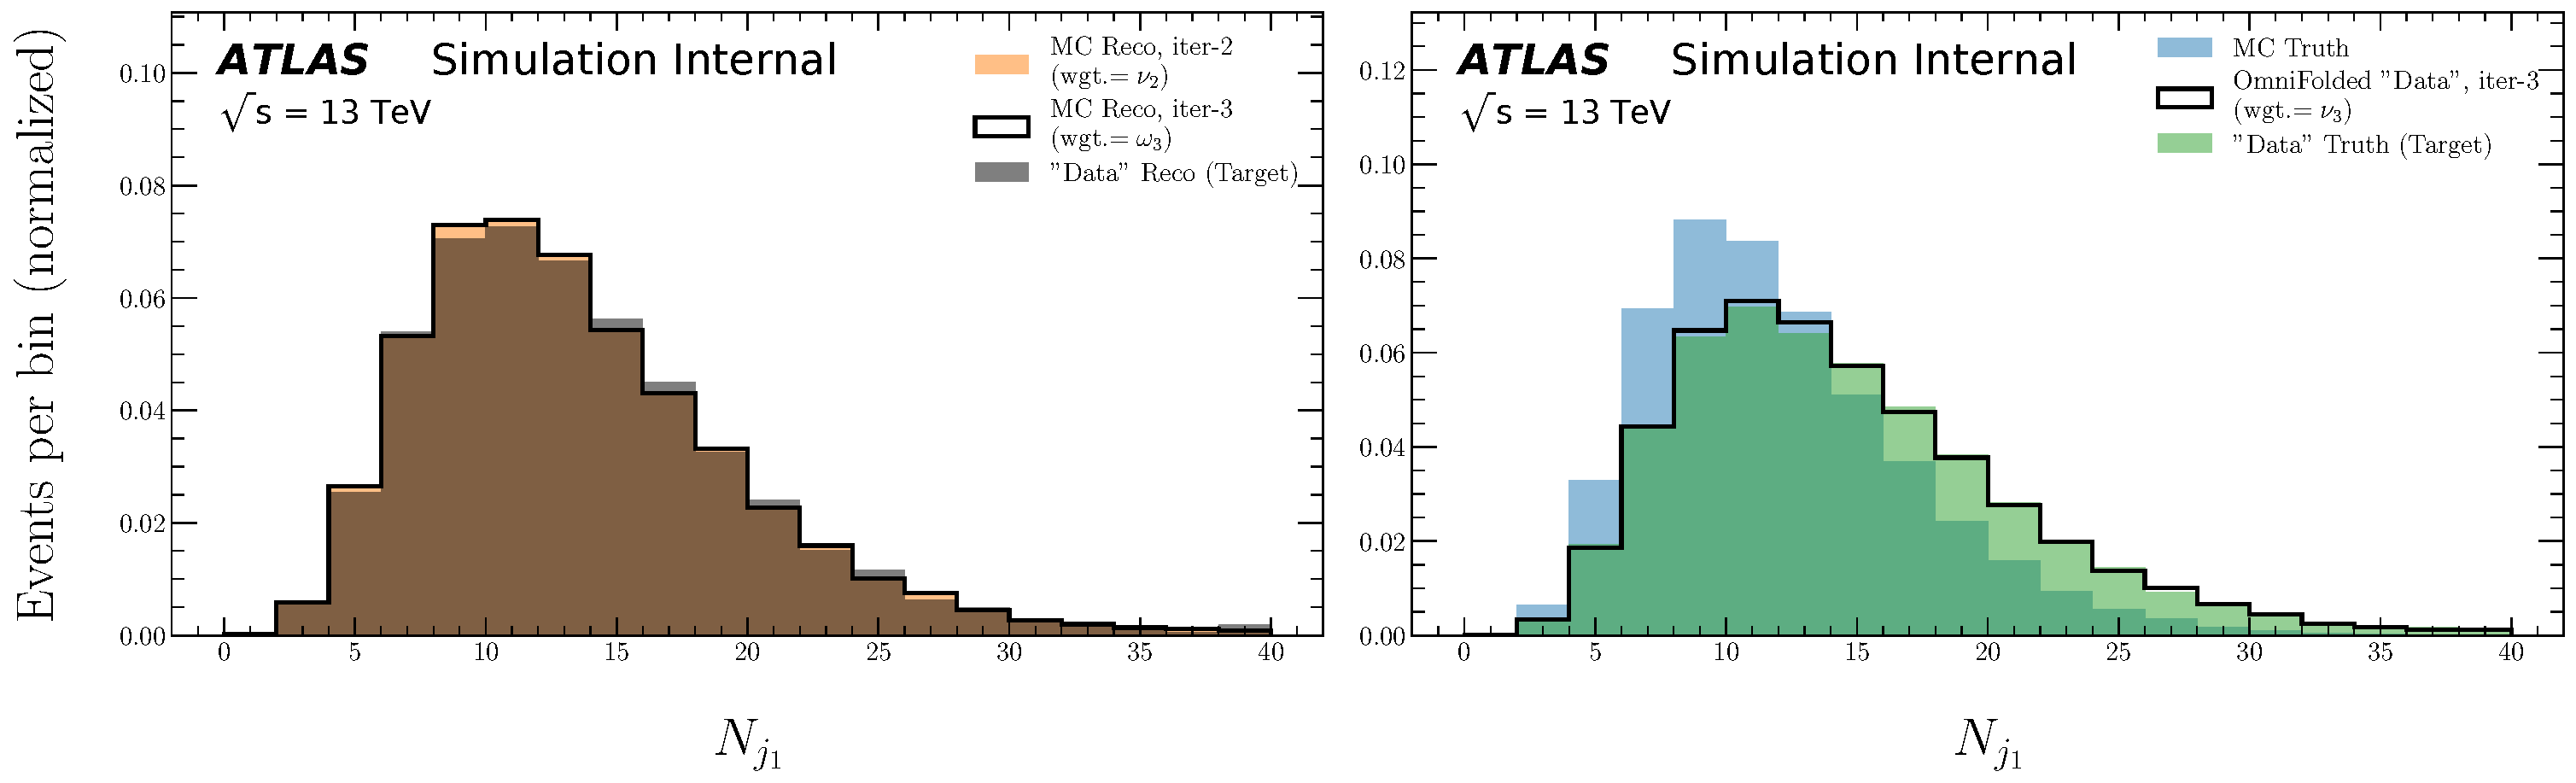
\includegraphics[width=0.85\textwidth]{figures/ATLASOmniFold-StressTest/ATLASOmniFold-StressTestA/MultiFold/Ntracks_trackj1/ATLASOmniFold-StressTestA-MultiFold-Ntracks_trackj1-Iteration03}}\\
\subfloat[After 4 iterations]{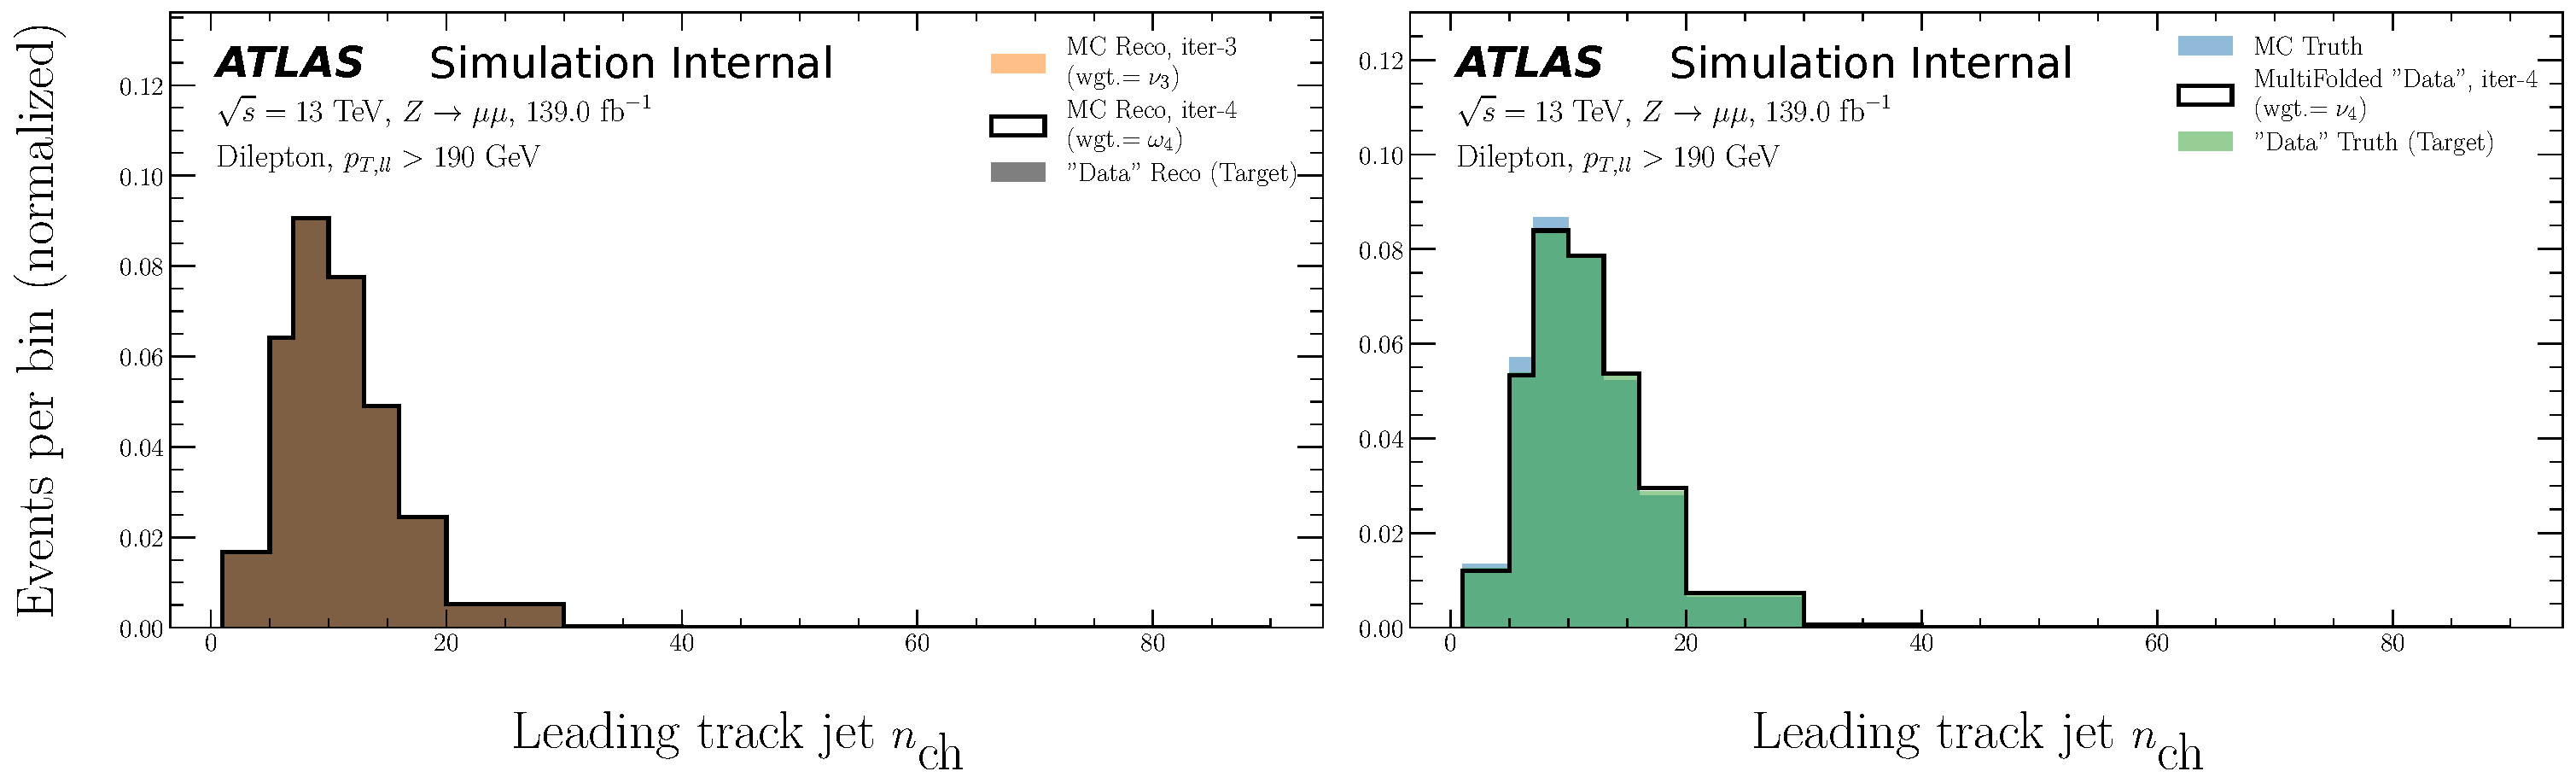
\includegraphics[width=0.85\textwidth]{figures/ATLASOmniFold-StressTest/ATLASOmniFold-StressTestA/MultiFold/Ntracks_trackj1/ATLASOmniFold-StressTestA-MultiFold-Ntracks_trackj1-Iteration04}}\\
\subfloat[After 5 iterations]{\includegraphics[width=0.85\textwidth]{figures/ATLASOmniFold-StressTest/ATLASOmniFold-StressTestA/MultiFold/Ntracks_trackj1/ATLASOmniFold-StressTestA-MultiFold-Ntracks_trackj1-Iteration05}}\\
\subfloat[After 6 iterations]{\includegraphics[width=0.85\textwidth]{figures/ATLASOmniFold-StressTest/ATLASOmniFold-StressTestA/MultiFold/Ntracks_trackj1/ATLASOmniFold-StressTestA-MultiFold-Ntracks_trackj1-Iteration06}}
\caption{A stress test for MultiFold using deterministic weights applied to the leading track jet constituent multiplicity.}
\label{fig:stressa_Ntracks_trackj1Multi}
\end{figure}

\clearpage

\subsubsection{Stochastic Weights}
\label{sec:stress:stochastic}

For a given event $x$ in sample $X$, the stress weights are given by

\begin{align}
\label{eq:stressBweights}
w = w_{MC}\,|\mathcal{N}(0, \sigma((\mathcal{Z}(x))))|\,,
\end{align}
%
where $w_{MC}$ is the Monte Carlo event weight, $\mathcal{Z}$ gives the z-score of $x\in X$, and $\sigma$ is the sigmoid function $\sigma(x)=\frac{1}{1 + e^{-x}}$.  We do a basic weight standardization given all stress weights $W$ by doing $w\mapsto\frac{w}{\langle W\rangle}$. These stress weights are constructed to induce a right shift in the given distribution.  Note these stress weights are based on a random variable, unlike the ones in Sec.~\ref{sec:stress:deterministic}.

\paragraph{UniFold}

Figures~\ref{fig:stressb_mass} and~\ref{fig:stressb_Ntracks_trackj1} are examples for the leading track jet mass and the number of tracks inside jets.  Additional examples can be found in App~\ref{sec:stressBunifolddet}.

\begin{figure}[h!]
\centering
\subfloat[Weights]{\includegraphics[width=0.45\textwidth]{figures/ATLASOmniFold-StressTest/ATLASOmniFold-StressTestB/UniFold/m_trackj1/ATLASOmniFold-StressTestB-UniFold-m_trackj1-StressWeightsHist.pdf}}\\
\subfloat[Input histograms]{\includegraphics[width=0.85\textwidth]{figures/ATLASOmniFold-StressTest/ATLASOmniFold-StressTestB/UniFold/m_trackj1/ATLASOmniFold-StressTestB-UniFold-m_trackj1-Distributions}}\\
\subfloat[After 1 iteration]{\includegraphics[width=0.85\textwidth]{figures/ATLASOmniFold-StressTest/ATLASOmniFold-StressTestB/UniFold/m_trackj1/ATLASOmniFold-StressTestB-UniFold-m_trackj1-Iteration01}}\\
\subfloat[After 2 iterations]{\includegraphics[width=0.85\textwidth]{figures/ATLASOmniFold-StressTest/ATLASOmniFold-StressTestB/UniFold/m_trackj1/ATLASOmniFold-StressTestB-UniFold-m_trackj1-Iteration02}}
\phantomcaption
\end{figure}

\begin{figure}[h!]
\centering
\ContinuedFloat
\subfloat[After 3 iterations]{\includegraphics[width=0.85\textwidth]{figures/ATLASOmniFold-StressTest/ATLASOmniFold-StressTestB/UniFold/m_trackj1/ATLASOmniFold-StressTestB-UniFold-m_trackj1-Iteration03}}\\
\subfloat[After 4 iterations]{\includegraphics[width=0.85\textwidth]{figures/ATLASOmniFold-StressTest/ATLASOmniFold-StressTestB/UniFold/m_trackj1/ATLASOmniFold-StressTestB-UniFold-m_trackj1-Iteration04}}\\
\subfloat[After 5 iterations]{\includegraphics[width=0.85\textwidth]{figures/ATLASOmniFold-StressTest/ATLASOmniFold-StressTestB/UniFold/m_trackj1/ATLASOmniFold-StressTestB-UniFold-m_trackj1-Iteration05}}\\
\subfloat[After 6 iterations]{\includegraphics[width=0.85\textwidth]{figures/ATLASOmniFold-StressTest/ATLASOmniFold-StressTestB/UniFold/m_trackj1/ATLASOmniFold-StressTestB-UniFold-m_trackj1-Iteration06}}
\caption{A stress test for UniFold applied to the leading track jet mass.}
\label{fig:stressb_mass}
\end{figure}

\begin{figure}[h!]
\centering
\subfloat[Weights]{\includegraphics[width=0.45\textwidth]{figures/ATLASOmniFold-StressTest/ATLASOmniFold-StressTestB/UniFold/Ntracks_trackj1/ATLASOmniFold-StressTestB-UniFold-Ntracks_trackj1-StressWeightsHist.pdf}}\\
\subfloat[Input histograms]{\includegraphics[width=0.85\textwidth]{figures/ATLASOmniFold-StressTest/ATLASOmniFold-StressTestB/UniFold/Ntracks_trackj1/ATLASOmniFold-StressTestB-UniFold-Ntracks_trackj1-Distributions}}\\
\subfloat[After 1 iteration]{\includegraphics[width=0.85\textwidth]{figures/ATLASOmniFold-StressTest/ATLASOmniFold-StressTestB/UniFold/Ntracks_trackj1/ATLASOmniFold-StressTestB-UniFold-Ntracks_trackj1-Iteration01}}\\
\subfloat[After 2 iterations]{\includegraphics[width=0.85\textwidth]{figures/ATLASOmniFold-StressTest/ATLASOmniFold-StressTestB/UniFold/Ntracks_trackj1/ATLASOmniFold-StressTestB-UniFold-Ntracks_trackj1-Iteration02}}
\phantomcaption
\end{figure}

\begin{figure}[h!]
\centering
\ContinuedFloat
\subfloat[After 3 iterations]{\includegraphics[width=0.85\textwidth]{figures/ATLASOmniFold-StressTest/ATLASOmniFold-StressTestB/UniFold/Ntracks_trackj1/ATLASOmniFold-StressTestB-UniFold-Ntracks_trackj1-Iteration03}}\\
\subfloat[After 4 iterations]{\includegraphics[width=0.85\textwidth]{figures/ATLASOmniFold-StressTest/ATLASOmniFold-StressTestB/UniFold/Ntracks_trackj1/ATLASOmniFold-StressTestB-UniFold-Ntracks_trackj1-Iteration04}}\\
\subfloat[After 5 iterations]{\includegraphics[width=0.85\textwidth]{figures/ATLASOmniFold-StressTest/ATLASOmniFold-StressTestB/UniFold/Ntracks_trackj1/ATLASOmniFold-StressTestB-UniFold-Ntracks_trackj1-Iteration05}}\\
\subfloat[After 6 iterations]{\includegraphics[width=0.85\textwidth]{figures/ATLASOmniFold-StressTest/ATLASOmniFold-StressTestB/UniFold/Ntracks_trackj1/ATLASOmniFold-StressTestB-UniFold-Ntracks_trackj1-Iteration06}}
\caption{A stress test for UniFold applied to the leading track jet constituent multiplicity.}
\label{fig:stressb_Ntracks_trackj1}
\end{figure}

\clearpage

\paragraph{MultiFold} Stress weights for the 16-dimensional MultiFold are shown in Fig.~\ref{fig:stressb_weightsMulti}.  These are constructed by adding the stress weights for each observable as defined by Eq.~\ref{eq:stressBweights} (the MC weight only enters once).  Figures~\ref{fig:stressb_massMultih} and~\ref{fig:stressb_Ntracks_trackj1Multi} are examples for the leading track jet mass and the number of tracks inside jets.  Additional examples can be found in App~\ref{sec:stressBmultifolddet}.

\begin{figure}[h!]
\centering
\subfloat[Weights]{\includegraphics[width=0.45\textwidth]{figures/ATLASOmniFold-StressTest/ATLASOmniFold-StressTestB/MultiFold/ATLASOmniFold-StressTestB-MultiFold--StressWeightsHist.pdf}}
\caption{A stress weights for the deterministic weight option for MultiFold.  Unlike UniFold, there is now only one set of weights for all 16 observables instead of a different set of weights for each observable.}
\label{fig:stressb_weightsMulti}
\end{figure}

\begin{figure}[h!]
\centering
\subfloat[Input histograms]{\includegraphics[width=0.85\textwidth]{figures/ATLASOmniFold-StressTest/ATLASOmniFold-StressTestB/MultiFold/m_trackj1/ATLASOmniFold-StressTestB-MultiFold-m_trackj1-Distributions}}\\
\subfloat[After 1 iteration]{\includegraphics[width=0.85\textwidth]{figures/ATLASOmniFold-StressTest/ATLASOmniFold-StressTestB/MultiFold/m_trackj1/ATLASOmniFold-StressTestB-MultiFold-m_trackj1-Iteration01}}\\
\subfloat[After 2 iterations]{\includegraphics[width=0.85\textwidth]{figures/ATLASOmniFold-StressTest/ATLASOmniFold-StressTestB/MultiFold/m_trackj1/ATLASOmniFold-StressTestB-MultiFold-m_trackj1-Iteration02}}
\phantomcaption
\end{figure}

\begin{figure}[h!]
\centering
\ContinuedFloat
\subfloat[After 3 iterations]{\includegraphics[width=0.85\textwidth]{figures/ATLASOmniFold-StressTest/ATLASOmniFold-StressTestB/MultiFold/m_trackj1/ATLASOmniFold-StressTestB-MultiFold-m_trackj1-Iteration03}}\\
\subfloat[After 4 iterations]{\includegraphics[width=0.85\textwidth]{figures/ATLASOmniFold-StressTest/ATLASOmniFold-StressTestB/MultiFold/m_trackj1/ATLASOmniFold-StressTestB-MultiFold-m_trackj1-Iteration04}}\\
\subfloat[After 5 iterations]{\includegraphics[width=0.85\textwidth]{figures/ATLASOmniFold-StressTest/ATLASOmniFold-StressTestB/MultiFold/m_trackj1/ATLASOmniFold-StressTestB-MultiFold-m_trackj1-Iteration05}}\\
\subfloat[After 6 iterations]{\includegraphics[width=0.85\textwidth]{figures/ATLASOmniFold-StressTest/ATLASOmniFold-StressTestB/MultiFold/m_trackj1/ATLASOmniFold-StressTestB-MultiFold-m_trackj1-Iteration06}}
\caption{A stress test for MultiFold using deterministic weights applied to the leading track jet mass.}
\label{fig:stressb_massMultih}
\end{figure}

\begin{figure}[h!]
\centering
\subfloat[Input histograms]{\includegraphics[width=0.85\textwidth]{figures/ATLASOmniFold-StressTest/ATLASOmniFold-StressTestB/MultiFold/Ntracks_trackj1/ATLASOmniFold-StressTestB-MultiFold-Ntracks_trackj1-Distributions}}\\
\subfloat[After 1 iteration]{\includegraphics[width=0.85\textwidth]{figures/ATLASOmniFold-StressTest/ATLASOmniFold-StressTestB/MultiFold/Ntracks_trackj1/ATLASOmniFold-StressTestB-MultiFold-Ntracks_trackj1-Iteration01}}\\
\subfloat[After 2 iterations]{\includegraphics[width=0.85\textwidth]{figures/ATLASOmniFold-StressTest/ATLASOmniFold-StressTestB/MultiFold/Ntracks_trackj1/ATLASOmniFold-StressTestB-MultiFold-Ntracks_trackj1-Iteration02}}
\phantomcaption
\end{figure}

\begin{figure}[h!]
\centering
\ContinuedFloat
\subfloat[After 3 iterations]{\includegraphics[width=0.85\textwidth]{figures/ATLASOmniFold-StressTest/ATLASOmniFold-StressTestB/MultiFold/Ntracks_trackj1/ATLASOmniFold-StressTestB-MultiFold-Ntracks_trackj1-Iteration03}}\\
\subfloat[After 4 iterations]{\includegraphics[width=0.85\textwidth]{figures/ATLASOmniFold-StressTest/ATLASOmniFold-StressTestB/MultiFold/Ntracks_trackj1/ATLASOmniFold-StressTestB-MultiFold-Ntracks_trackj1-Iteration04}}\\
\subfloat[After 5 iterations]{\includegraphics[width=0.85\textwidth]{figures/ATLASOmniFold-StressTest/ATLASOmniFold-StressTestB/MultiFold/Ntracks_trackj1/ATLASOmniFold-StressTestB-MultiFold-Ntracks_trackj1-Iteration05}}\\
\subfloat[After 6 iterations]{\includegraphics[width=0.85\textwidth]{figures/ATLASOmniFold-StressTest/ATLASOmniFold-StressTestB/MultiFold/Ntracks_trackj1/ATLASOmniFold-StressTestB-MultiFold-Ntracks_trackj1-Iteration06}}
\caption{A stress test for MultiFold using deterministic weights applied to the leading track jet constituent multiplicity.}
\label{fig:stressb_Ntracks_trackj1Multi}
\end{figure}

\clearpage

\subsection{Model Dependence}
\label{sec:modeldep}

In this section, we unfold Sherpa with Pythia. Up to six iterations are shown, based on the study detailed in Appendix~\ref{sec:num_iterations} that demonstrates that unfolding Sherpa with Pythia via UniFold performs best after around 5 iterations. 

\paragraph{UniFold}

Figures~\ref{fig:stressc_mass} and~\ref{fig:stressc_Ntracks_trackj1} are examples for the leading track jet mass and the number of tracks inside jets.  Additional examples can be found in App~\ref{sec:stresscunifolddet}.

\begin{figure}[h!]
\centering
\subfloat[Input histograms]{\includegraphics[width=0.85\textwidth]{figures/ATLASOmniFold-StressTest/ATLASOmniFold-StressTestC/UniFold/m_trackj1/ATLASOmniFold-StressTestC-UniFold-m_trackj1-Distributions}}\\
\subfloat[After 1 iteration]{\includegraphics[width=0.85\textwidth]{figures/ATLASOmniFold-StressTest/ATLASOmniFold-StressTestC/UniFold/m_trackj1/ATLASOmniFold-StressTestC-UniFold-m_trackj1-Iteration01}}\\
\subfloat[After 2 iterations]{\includegraphics[width=0.85\textwidth]{figures/ATLASOmniFold-StressTest/ATLASOmniFold-StressTestC/UniFold/m_trackj1/ATLASOmniFold-StressTestC-UniFold-m_trackj1-Iteration02}}
\phantomcaption
\end{figure}

\begin{figure}[h!]
\centering
\ContinuedFloat
\subfloat[After 3 iterations]{\includegraphics[width=0.85\textwidth]{figures/ATLASOmniFold-StressTest/ATLASOmniFold-StressTestC/UniFold/m_trackj1/ATLASOmniFold-StressTestC-UniFold-m_trackj1-Iteration03}}\\
\subfloat[After 4 iterations]{\includegraphics[width=0.85\textwidth]{figures/ATLASOmniFold-StressTest/ATLASOmniFold-StressTestC/UniFold/m_trackj1/ATLASOmniFold-StressTestC-UniFold-m_trackj1-Iteration04}}\\
\subfloat[After 5 iterations]{\includegraphics[width=0.85\textwidth]{figures/ATLASOmniFold-StressTest/ATLASOmniFold-StressTestC/UniFold/m_trackj1/ATLASOmniFold-StressTestC-UniFold-m_trackj1-Iteration05}}\\
\subfloat[After 6 iterations]{\includegraphics[width=0.85\textwidth]{figures/ATLASOmniFold-StressTest/ATLASOmniFold-StressTestC/UniFold/m_trackj1/ATLASOmniFold-StressTestC-UniFold-m_trackj1-Iteration06}}
\caption{UniFolding Sherpa with Pythia for the leading track jet mass.}
\label{fig:stressc_mass}
\end{figure}

\begin{figure}[h!]
\centering
\subfloat[Input histograms]{\includegraphics[width=0.85\textwidth]{figures/ATLASOmniFold-StressTest/ATLASOmniFold-StressTestC/UniFold/Ntracks_trackj1/ATLASOmniFold-StressTestC-UniFold-Ntracks_trackj1-Distributions}}\\
\subfloat[After 1 iteration]{\includegraphics[width=0.85\textwidth]{figures/ATLASOmniFold-StressTest/ATLASOmniFold-StressTestC/UniFold/Ntracks_trackj1/ATLASOmniFold-StressTestC-UniFold-Ntracks_trackj1-Iteration01}}\\
\subfloat[After 2 iterations]{\includegraphics[width=0.85\textwidth]{figures/ATLASOmniFold-StressTest/ATLASOmniFold-StressTestC/UniFold/Ntracks_trackj1/ATLASOmniFold-StressTestC-UniFold-Ntracks_trackj1-Iteration02}}
\phantomcaption
\end{figure}

\begin{figure}[h!]
\centering
\ContinuedFloat
\subfloat[After 3 iterations]{\includegraphics[width=0.85\textwidth]{figures/ATLASOmniFold-StressTest/ATLASOmniFold-StressTestC/UniFold/Ntracks_trackj1/ATLASOmniFold-StressTestC-UniFold-Ntracks_trackj1-Iteration03}}\\
\subfloat[After 4 iterations]{\includegraphics[width=0.85\textwidth]{figures/ATLASOmniFold-StressTest/ATLASOmniFold-StressTestC/UniFold/Ntracks_trackj1/ATLASOmniFold-StressTestC-UniFold-Ntracks_trackj1-Iteration04}}\\
\subfloat[After 5 iterations]{\includegraphics[width=0.85\textwidth]{figures/ATLASOmniFold-StressTest/ATLASOmniFold-StressTestC/UniFold/Ntracks_trackj1/ATLASOmniFold-StressTestC-UniFold-Ntracks_trackj1-Iteration05}}\\
\subfloat[After 6 iterations]{\includegraphics[width=0.85\textwidth]{figures/ATLASOmniFold-StressTest/ATLASOmniFold-StressTestC/UniFold/Ntracks_trackj1/ATLASOmniFold-StressTestC-UniFold-Ntracks_trackj1-Iteration06}}
\caption{UniFolding Sherpa with Pythia forthe leading track jet constituent multiplicity.}
\label{fig:stressc_Ntracks_trackj1}
\end{figure}

\clearpage

\paragraph{MultiFold} Figures~\ref{fig:stressc_massMultih} and~\ref{fig:stressc_Ntracks_trackj1Multi} are examples for the leading track jet mass and the number of tracks inside jets.  Additional examples can be found in App~\ref{sec:stresscmultifolddet}.

\begin{figure}[h!]
\centering
\subfloat[Input histograms]{\includegraphics[width=0.85\textwidth]{figures/ATLASOmniFold-StressTest/ATLASOmniFold-StressTestC/MultiFold/m_trackj1/ATLASOmniFold-StressTestC-MultiFold-m_trackj1-Distributions}}\\
\subfloat[After 1 iteration]{\includegraphics[width=0.85\textwidth]{figures/ATLASOmniFold-StressTest/ATLASOmniFold-StressTestC/MultiFold/m_trackj1/ATLASOmniFold-StressTestC-MultiFold-m_trackj1-Iteration01}}\\
\subfloat[After 2 iterations]{\includegraphics[width=0.85\textwidth]{figures/ATLASOmniFold-StressTest/ATLASOmniFold-StressTestC/MultiFold/m_trackj1/ATLASOmniFold-StressTestC-MultiFold-m_trackj1-Iteration02}}
\phantomcaption
\end{figure}

\begin{figure}[h!]
\centering
\ContinuedFloat
\subfloat[After 3 iterations]{\includegraphics[width=0.85\textwidth]{figures/ATLASOmniFold-StressTest/ATLASOmniFold-StressTestC/MultiFold/m_trackj1/ATLASOmniFold-StressTestC-MultiFold-m_trackj1-Iteration03}}\\
\subfloat[After 4 iterations]{\includegraphics[width=0.85\textwidth]{figures/ATLASOmniFold-StressTest/ATLASOmniFold-StressTestC/MultiFold/m_trackj1/ATLASOmniFold-StressTestC-MultiFold-m_trackj1-Iteration04}}\\
\subfloat[After 5 iterations]{\includegraphics[width=0.85\textwidth]{figures/ATLASOmniFold-StressTest/ATLASOmniFold-StressTestC/MultiFold/m_trackj1/ATLASOmniFold-StressTestC-MultiFold-m_trackj1-Iteration05}}\\
\subfloat[After 6 iterations]{\includegraphics[width=0.85\textwidth]{figures/ATLASOmniFold-StressTest/ATLASOmniFold-StressTestC/MultiFold/m_trackj1/ATLASOmniFold-StressTestC-MultiFold-m_trackj1-Iteration06}}
\caption{MultiFolding Sherpa with Pythia for the leading track jet mass.}
\label{fig:stressc_massMultih}
\end{figure}

\begin{figure}[h!]
\centering
\subfloat[Input histograms]{\includegraphics[width=0.85\textwidth]{figures/ATLASOmniFold-StressTest/ATLASOmniFold-StressTestC/MultiFold/Ntracks_trackj1/ATLASOmniFold-StressTestC-MultiFold-Ntracks_trackj1-Distributions}}\\
\subfloat[After 1 iteration]{\includegraphics[width=0.85\textwidth]{figures/ATLASOmniFold-StressTest/ATLASOmniFold-StressTestC/MultiFold/Ntracks_trackj1/ATLASOmniFold-StressTestC-MultiFold-Ntracks_trackj1-Iteration01}}\\
\subfloat[After 2 iterations]{\includegraphics[width=0.85\textwidth]{figures/ATLASOmniFold-StressTest/ATLASOmniFold-StressTestC/MultiFold/Ntracks_trackj1/ATLASOmniFold-StressTestC-MultiFold-Ntracks_trackj1-Iteration02}}
\phantomcaption
\end{figure}

\begin{figure}[h!]
\centering
\ContinuedFloat
\subfloat[After 3 iterations]{\includegraphics[width=0.85\textwidth]{figures/ATLASOmniFold-StressTest/ATLASOmniFold-StressTestC/MultiFold/Ntracks_trackj1/ATLASOmniFold-StressTestC-MultiFold-Ntracks_trackj1-Iteration03}}\\
\subfloat[After 4 iterations]{\includegraphics[width=0.85\textwidth]{figures/ATLASOmniFold-StressTest/ATLASOmniFold-StressTestC/MultiFold/Ntracks_trackj1/ATLASOmniFold-StressTestC-MultiFold-Ntracks_trackj1-Iteration04}}\\
\subfloat[After 5 iterations]{\includegraphics[width=0.85\textwidth]{figures/ATLASOmniFold-StressTest/ATLASOmniFold-StressTestC/MultiFold/Ntracks_trackj1/ATLASOmniFold-StressTestC-MultiFold-Ntracks_trackj1-Iteration05}}\\
\subfloat[After 6 iterations]{\includegraphics[width=0.85\textwidth]{figures/ATLASOmniFold-StressTest/ATLASOmniFold-StressTestC/MultiFold/Ntracks_trackj1/ATLASOmniFold-StressTestC-MultiFold-Ntracks_trackj1-Iteration06}}
\caption{MultiFolding Sherpa with Pythia for the leading track jet constituent multiplicity.}
\label{fig:stressc_Ntracks_trackj1Multi}
\end{figure}

\clearpage

\subsubsection{Neural Network Initialization Sensitivity}
\label{sec:modeldep:NNinit}
To determine the sensitivity of neural network initialization, we run the unfolding procedure for 100 different random initializations (for each observable's UniFold and MultiFold on all observables) to produce 100 different sets of weights.  Then after choosing some binning, we generate 100 different histograms based on these weights.  Finally, we take the average and standard deviation of the bin contents to probe the sensitivity to initialization.  \textbf{show unfolding results with error bars below}

\subsubsection{Bootstrapping for Statistical Uncertainty}
\label{sec:modeldep:bootstrap}
To determine the effect of statistical uncertainty in the "data", we first take 100 bootstrapped samples from the "data" sample and then run all the unfolding procedures for each one to again produce 100 different sets of weights.  As above, after choosing some binning, we generate 100 different histograms based on these weights.  Then, we take the average and standard deviation of the bin contents to probe the effect of statistical uncertainty.  Note that we inadvertently take into account neural network initialization sensitivity as well, as we initialize a new model for each unfolding run.  Thus, one can see that compared to the sensitively to initialization (shown above), the effect of statistical uncertainty in the "data" sample is small, as the increase in bin contents standard deviation is marginal at best. \textbf{show unfolding results with error bars below}
